%
% Modified version of the sample_ndthesis.tex
% by Sameer Vijay
% Last Change: Wed Jul 27 2005 14:00 CEST
%
%%%%%%%%%%%%%%%%%%%%%%%%%%%%%%%%%%%%%%%%%%%%%%%%%%%%%%%%%%%%%%%%%%%%%%%%
%
% Sample Notre Dame Thesis/Dissertation
% Using Donald Peterson's ndthesis classfile
%
% Written by Jeff Squyres and Don Peterson
%
% Provided by the Information Technology Committee of
%   the Graduate Student Union
%   http://www.gsu.nd.edu/
%
% Nothing in this document is serious except the format.  :-)
%
%%%%%%%%%%%%%%%%%%%%%%%%%%%%%%%%%%%%%%%%%%%%%%%%%%%%%%%%%%%%%%%%%%%%%%%%
% This is *not* a substitute for Donald's orginial documentation.  See
% /afs/nd.edu/usr/local/src/tex/texmf/doc/latex/ndthesis/ndthesis.dvi
% for documentation on the particular commands and whatnot.
%%%%%%%%%%%%%%%%%%%%%%%%%%%%%%%%%%%%%%%%%%%%%%%%%%%%%%%%%%%%%%%%%%%%%%%%
%
% You should *also* have a ND formatting guide to ensure that you have
% all the relevant parts, put the captions in the right place, etc.
% Just because you have this wonderful style classfile doesn't mean
% that it removes *all* the formatting onus from you.  :-)
%
% Normally, you should break all of this stuff up into separate files
% (at the very least, one chapter per file) and use the \input
% command.  This is all one file for brevity's (and clarity's) sake.
%
% Note that you should also have a good Makefile; one that invokes
% LaTeX as many times as necessary (up to 4) and bibtex if necessary.
% One should be included in this distribution.  You may want to modify
% the Makefile to make separate chapters, if necessary.
%
% If you have any suggestions, comments, questions, please send e-mail
% to: ndthesis@gsu.nd.edu
%
%%%%%%%%%%%%%%%%%%%%%%%%%%%%%%%%%%%%%%%%%%%%%%%%%%%%%%%%%%%%%%%%%%%%%%%%

%\documentclass[textrefs,review]{nddiss2e}
\documentclass[textrefs,final,noinfo,12pt]{nddiss2e}

\usepackage[lofdepth,lotdepth]{subfig}
\usepackage{floatrow}
%\usepackage{epsfig}
\usepackage{graphicx}
%\usepackage{epstopdf}
%\usepackage[pdf]{pstricks}
%\usepackage{adjustbox}
\usepackage{booktabs}
\usepackage{xspace}
\usepackage{comment}
\usepackage{amsmath}
\usepackage{caption}
\usepackage{rotating}

\newcommand{\fig}{Figure\xspace}
\newcommand{\tab}{Table\xspace}
\newcommand{\sect}{Section\xspace}
\newcommand{\chap}{Chapter\xspace}
\newcommand{\eqn}{Equation\xspace}
\newcommand{\app}{Appendix\xspace}
\newcommand{\Ge}[1]{$^{#1}$Ge\xspace}
\newcommand{\As}[1]{$^{#1}$As\xspace}
\newcommand{\Se}[1]{$^{#1}$Se\xspace}
\newcommand{\Mg}[1]{$^{#1}$Mg\xspace}
\newcommand{\Si}[1]{$^{#1}$Si\xspace}
\newcommand{\He}[1]{$^{#1}$He\xspace}
\newcommand{\GeTargets}{$^{74,76}$Ge\xspace}
\newcommand{\SeProducts}{$^{76,78}$Se\xspace}
\newcommand{\reaction}{$^{74,76}$Ge($^3$He,n)$^{76,78}$Se\xspace}
\newcommand{\MgReaction}{$^{26}$Mg($^3$He,n)$^{28}$Si\xspace}
\newcommand{\DuReaction}{d(d,n)$^3$He\xspace}
\newcommand{\zvbb}{$0\nu\beta\beta$\xspace}
\newcommand{\NME}{$M^{0\nu}$\xspace}
\newcommand{\zp}{$0^+$\xspace}
\bibpunct{[}{]}{,}{n}{}{;}
% % uncomment the following line 
% if using chapter-wise bibliography
% \usepackage{chapterbib}
% \renewcommand{\bibname}{Cited Works}
% \renewcommand{\bibsection}{\section{\bibname}}

\begin{document}

\frontmatter

\title{TWO-PROTON TRANSFER ONTO GE \\ {\small\scshape HELPING OUT THE NEUTRINO PEOPLE} }
\author{Amy Roberts}
\work{Dissertation}
\degprior{B.S.}
\degaward{Doctor of Philosophy\\in\\Physics}
\advisor{James Kolata}
% \secondadvisor{Gordon Gray}
\department{Physics}

\maketitle
%%%%%%%%%%%%%%%%%%%%%%%%%%%%%%%%%%%%%%%%%%%%%%%%%%%%%%%%%%%%%%%%%%%%%%%%
%
% Front stuff
%
%%%%%%%%%%%%%%%%%%%%%%%%%%%%%%%%%%%%%%%%%%%%%%%%%%%%%%%%%%%%%%%%%%%%%%%%

\copyrightholder{Amy Roberts}
\copyrightyear{2013}
\makecopyright

\begin{abstract}
A great deal of effort has gone into detecting neutrinoless double beta decay (\zvbb).  But the nuclei that offer the greatest chance of observing this phenomenon are poorly understood.  While an observation of \zvbb has dramatic implications all by itself, there are compelling reasons to better understand the nuclei that might play host to such an event.  The nucleus affects the rate of such an event, important in planning experiments.  And should \zvbb be detected, the nucleus must be well-understood to extract parameters such as the absolute mass scale of the neutrino.

For many years, the nuclear community has worked to piece together a clearer understanding of these nuclei using single-nucleon transfer reactions.  Two-nucleon transfer reactions are also of fundamental importance.  This work investigates two-proton transfer onto \Ge{76} and \Ge{78}.
\end{abstract}

\renewcommand{\dedicationname}{New Dedication Name}

\begin{dedication}
  To George, my favorite Gnu
\end{dedication}

\tableofcontents
\listoffigures
\listoftables

\begin{preface}
  Nuclear physics has been working had for decades to better understand the Nuclear Matrix Elements (NME) of nuclei used in \zvbb studies.  The field has made significant strides; where first it was thought that data from neutrino-full double beta decay provided sufficient information, subsequent theory work showed that this was not the case.  Since then, exhaustive assays of single-nucleon transfers have contributed significantly to the understanding of nucleon occupancy (spoiler alert - it's more complicated than we'd like), and with the guidance of theorists, have begun exploring two-nucleon transfer reactions to better understand correlations between nucleons within these nuclei.  This experiment is the final two-nucleon transfer reaction for the Ge isotope.

  What this thesis will do is present the data from the transfer reaction.  What this thesis will not do is explain how this affects \zvbb.
\end{preface}

\begin{acknowledge}
  I would like to thank the Notre Dame community, particularly the physics department and health services, who kept me well and worked hard to teach me some physics.  I would also like to thank my advisor, Dr.\ James Kolata, without
  whom this work would not have been possible.

  Finally, I would like to thank the U.S.\ Government, Department of
  Gnus, for their generous grant, number GNU3042920920.3, which
  allowed me to pursue my work.
\end{acknowledge}

\begin{symbols}
  \sym{\mathcal{F}}{sighting frequency of Gnus about campus}
  \sym{p}{student population}
  \sym{f}{type of food available}
  \sym{d}{day of week}
  \sym{c}{speed of light}
  \sym{m}{mass}
  \sym{e}{elementary charge}
  \sym{a,b}{miscellaneous constants}  
  \sym{E}{energy}  
\end{symbols}

\mainmatter
\setcounter{chapter}{0}
%
% Chapter 1
%

%
% Modified by Sameer Vijay
% Last Change: Tue Jul 26 2005 13:00 CEST
%
%%%%%%%%%%%%%%%%%%%%%%%%%%%%%%%%%%%%%%%%%%%%%%%%%%%%%%%%%%%%%%%%%%%%%%%%
%
% Sample Notre Dame Thesis/Dissertation
% Using Donald Peterson's ndthesis classfile
%
% Written by Jeff Squyres and Don Peterson
%
% Provided by the Information Technology Committee of
%   the Graduate Student Union
%   http://www.gsu.nd.edu/
%
% Nothing in this document is serious except the format.  :-)
%
% If you have any suggestions, comments, questions, please send e-mail
% to: ndthesis@gsu.nd.edu
%
%%%%%%%%%%%%%%%%%%%%%%%%%%%%%%%%%%%%%%%%%%%%%%%%%%%%%%%%%%%%%%%%%%%%%%%%


%
% Chapter 1
%

\chapter{NEUTRINO PHYSICS AND ITS DEPENDENCE ON NUCLEAR PHYSICS}
\label{chap:0vbb}
\begin{comment}
Neutrino physics is fascinating because ??????.
Maybe I will talk about particles in general - but no, that's probably a bit too much.
I will mention the standard model table and talk about why neutrinos are important in physics today?

The neutrino was first proposed as a undetectable particle that carried away energy in nuclear decay processes \citep{Pauli}.  Twenty-six years later (fact check!), Reines and Cowan detected inverse beta decay to detect anti-neutrinos streaming out of a nearby nuclear reactor \citep{poltergeist}.  Detecting neutrinos is difficult: with an interaction volume of 10$^{26}$ potential targets, Reines and Cowan saw 1 event per week (FACT CHECK!!) \citep{poltergeist}.  Simply confirming the existence of the particle hypothesized to participate in beta decay was significant enough to merit the Nobel Prize \citep{CowanNobel}.

Figure: beta decay spectrum, with and without neutrino.  See F.A. Scott, Phys Rev 48, 391 (1935)

While detecting neutrinos is a difficult endeavor, it's also a lucrative one: particles that interact extremely rarely carry information about where they're created, no matter what they have to travel through to get to us.  With a detector that counts neutrinos, one can begin to imagine interrogating the cosmos: ``How many neutrinos are you making?  And you?  And you?''  Bahcall was interested in finding out how many neutrinos the Sun made.  And so he and Ray Davis set out to make a good neutrino counter. 

(AMY!  You're neglecting to talk about the experiment that demonstrated the left-handedness of neutrinos by Goldhaber in 1958.  This is kind of relevant to \zvbb!)
\end{comment}

The neutrino was first proposed by Pauli to be a chargeless, nearly massless fermion \citep{Pauli}.  This particle was a means to preserve energy, momentum, and angular momentum conservation in nuclear beta decay.  The hypothesized process taking place within the nucleus was
\begin{equation}
n \rightarrow p + e^- + \overline{v}_e,
\end{equation}
where a neutron $n$ decays into a proton $p$, an electron $e^-$, and also an electron anti-neutrino $\overline{v}_e$, allowing the continuous electron energy spectrum that was observed. The existence of this difficult-to-detect particle was not confirmed until 26 years later, when Reines and Cowan used a nuclear reactor as a source of anti-neutrinos and observed inverse beta decay of proton targets \citep{poltergeist}.  Since the first detection of electron anti-neutrinos, an much has been learned about these elusive particles.  This chapter will begin by discussing what is currently known about neutrinos, in particular that there are three, unique flavors and that while they are very light, they do have mass.  The remainder of the chapter discusses how neutrinos get their mass in the Standard Model (SM) framework and the experiments currently underway to help determine why the neutrino mass scale is so small.

\subsection{Neutrino Oscillation}
Neutrinos interact very weakly with matter, and while this makes their detection difficult, it also makes them a potentially valuable source of information.  Studying the interior of systems that produce neutrinos becomes possible with a neutrino detector, while other forms of radiation would be absorbed by the surrounding matter.  Raymond Davis and John Bahcall recognized the neutrino could be used to test the theory that nuclear fusion was the Sun's energy source.  The neutrino detector built by Davis consisted of 100,000 gallons of liquid dry cleaning fluid, which contained $^{37}$Cl \citep{DavisInitial}.  Solar neutrinos interacting with $^{37}$Cl initiate inverse beta decay, leaving the radioactive $^{37}$Ar as a detectable signal.  Years of careful data taking yielded a count of $\sim$7 neutrinos per two weeks \citep{DavisInitial}, only $\sim\frac{1}{3}$ the rate predicted by Bahcall \citep{BahcallSun}.  Further refinements to the experiment and to the calculations confirmed the discrepancy \citep{Davis}.

While the Davis experiment continued to collect data, other experiments were begun to explore other properties of the neutrino.  Originally imagined as a single particle, it was found that there are three distinct flavors of neutrinos, each associated with a lepton partner.  It is important to note that the beta decay which transforms nucleus $A$ to $A'$,
\begin{equation}
A(Z,N) \rightarrow A'(Z-1,N+1) + \overline{l} + v_l,
\end{equation}
where $l$ is an electron, muon, or tau, requires the mass difference between the initial and final nuclei to be larger than the mass of the lepton $l$.  While electrons have a mass of only 0.51~MeV, muons are considerably heavier, having a mass of 105.7~MeV.  Tau leptons have a mass of 1776.8~MeV, comparable to a light nucleus. At most, nuclear reactions in the Sun provide $\sim$11~MeV, so that the Sun can produce only electron neutrinos.  Energetic pion beams at Brookhaven National Laboratory (BNL) were used to make the first direct measurement of muon neutrinos \citep{muonNeutrino}.  Later, more than 25 years after the discovery of the tau lepton \citep{tauDiscovery} in 1975, tau neutrinos were successfully detected at Fermilab \citep{tauNeutrino}.  The inclusion of the neutrino into the SM as a participant in weak interactions mediated by the $W^{\pm}$ and $Z^0$ bosons suggested that experiments determining the lifetime of the $Z^0$ boson could determine the number of interacting neutrinos.  The $Z^0$ has known lepton and hadron decay modes \citep{PDG} and can also decay to a neutrino-antineutrino pair of any flavor provided the neutrinos have a mass less than $M_Z/2$.  More flavors of light neutrinos should therefore reduce the $Z^0$ lifetime while fewer should increase it.   An electron-positron collider experiment at CERN measured the lifetime of the $Z^0$ and determined the number of neutrino flavors to be $2.92\pm0.05$ \citep{PDG}.

That there are three flavors of neutrinos, each associated with a different-mass lepton, is significant because the Davis experiment was sensitive only to electron neutrinos.  Other radiochemical neutrino experiments, also only sensitive to electron neutrinos, confirmed Davis' results \citep{SNO_Sun,SuperK_Sun,PDG}.  An idea suggested by Pontecorvo, that neutrinos have mass \citep{Pontecorvo}, showed a way forward.  Neutrinos had been incorporated into the SM as massless, making it impossible for their flavor to vary with time.  If neutrinos were massive, neutrinos could change flavor.  The hypothesis was that the radiochemical experiments, sensitive only to electron neutrinos, were measuring a deficit because $\sim\frac{2}{3}$ of the electron neutrinos from the Sun had changed flavor and could not be detected.  SNO, an experiment designed to be sensitive to all three neutrino flavors, measured the predicted number of solar neutrinos \citep{SNO_Sun}, confirming that neutrino flavors change with time and therefore that neutrinos must be massive.

That neutrino flavor oscillation implies a massive neutrino is a general property of combining states with different energy eigenvalues.  This can be seen by imagining some two states, $\psi_{\alpha}$ and $\psi_{\beta}$, neither of which are energy eigenstates.  These states can be written in terms of the energy eigenstates: 
\begin{align}
|\psi_{\alpha}\rangle &= U_{\alpha 1}|\psi_1\rangle + U_{\alpha 2}|\psi_2\rangle \\
|\psi_{\beta}\rangle &= U_{{\beta}1}|\psi_1\rangle + U_{{\beta}2}|\psi_2\rangle, 
\end{align}
where $\hat{H}|\psi_1\rangle = E_1|\psi_1\rangle$ and $\hat{H}|\psi_2\rangle = E_2|\psi_2\rangle$.  Then for an initial state $|\psi_{\alpha}\rangle$, the probability of measuring $|\psi_{\beta}\rangle$ some time $t$ later is
\begin{align}
\begin{split}
P(\alpha\rightarrow\beta) &=  |\langle\psi_{\beta}|\hat{T}|\psi_{\alpha}\rangle|^2 \\
                             &=  |\langle\psi_{\beta}|e^{i\hat{H}t / \hbar}|\psi_{\alpha}\rangle|^2 \\
                             &=  U_{{\alpha}1}U_{{\alpha}2}U_{{\beta}1}U_{{\beta}2} \times \frac{\cos((E_1 - E_2)t/\hbar)}{2} 
\end{split}
\end{align}
This calculation is not exactly analogous to neutrino mixing because there are three mass eigentstates, not two.  However, the modulation of the probability of detecting a different flavor state is, as in this test case, dependent on the energy difference.  In the case of the neutrino, the energy eigenstates are also its mass eigenstates, and it can be shown that in vacuum, the neutrino oscillation phase between components $\nu_i$ and $\nu_j$ is \citep{PDG,neutrinoOscillations}
\begin{equation}
\phi = (m_i^2 - m_j^2)\frac{L}{2E},
\end{equation}
where $m_i$ and $m_j$ are the masses of $\nu_i$ and $\nu_j$, respectively, $L$ is the distance between the neutrino source and the detector, and $E$ is the neutrino energy.  Neutrino oscillation experiments are therefore sensitive to the differences between neutrino masses but not to the absolute mass scale.  It is important to note that the oscillation phase for neutrinos traveling through matter is still dependent only on the mass differences \citep{MSW}.  Cosmological measurements and beta-decay experiments, while not sensitive to neutrino oscillation, can place limits on the absolute neutrino mass scale.  Cosmological limits are sensitive to $m_1+m_2+m_3$ and constrain this quantity to be less than $0.3-1.3$~eV at the 95\% confidence level \citep{cosmoNuMassLimit}.  Experiments designed to measure the endpoint of beta decay are sensitive to the quantity $\sqrt{|U_{e1}|^2m_1^2 + |U_{e2}|^2m_2^2 + |U_{e3}|^2m_3^2}$ currently limit this value to less than 2.05~eV \citep{tritiumEndpoint}. 

The neutrino mixing matrix $U$ can be written with three angles, one Dirac CP-violating phase, and two Majorana CP-violating phases:
\begin{multline}
\begin{bmatrix}
c_{12}c_{13} & s_{12}c_{13} & s_{13}e^{-i\delta} \\
-s_{12}c_{23}-c_{12}s_{23}s_{13}e^{i\delta} & c_{12}c_{23}-s_{12}s_{23}s_{13}e^{i\delta} & s_{23}c_{13} \\
s_{12}s_{23}-c_{12}c_{23}s_{13}e^{i\delta} & -c_{12}s_{23}-s_{12}c_{23}s_{13}e^{i\delta} & c_{23}c_{13} 
\end{bmatrix} 
\\
\times 
\begin{bmatrix}
1 & 0 & 0 \\
0 & e^{\frac{i}{2}\alpha_{21}} & 0 \\
0 & 0 & e^{\frac{i}{2}\alpha_{31}}
\end{bmatrix}
,
\end{multline}
where $c_{ij} = \cos{\theta_{ij}}$ and $s_{ij} = \sin{\theta_{ij}}$, $\delta$ is the Dirac CP-violating phase, and the Majorana CP-violating phases $\alpha_{ij}$ are only relevant if the neutrino is a Majorana fermion as discussed in {\sect}~\ref{sec:mass}.  Several generations of long-baseline neutrino experiments using solar, atmospheric, and reactor neutrinos have constrained the mixing parameters and mass differences.  A summary of the parameters is given in {\tab}~\ref{tab:neutrinoParameters}.
\begin{table}
\ra{1.1}
%\centering
\begin{center}
\caption[\uppercase{Neutrino oscillation parameters}]{\\\uppercase{Neutrino oscillation parameters} \label{tab:neutrinoParameters}}
\begin{tabular}{lll}\toprule
Parameter & Best Fit ($\pm$ 1$\sigma$) & 3$\sigma$ \\
\midrule
${\Delta}m^2_{12}$ [$10^{-5}$ eV$^2$] & $7.58^{+0.22}_{-0.26}$ & 6.99 - 8.18 \\
$|{\Delta}m^2_{31}|$ [$10^{-3}$ eV$^2$] & $2.35^{+0.12}_{-0.09}$ & 2.06 - 2.67 \\
$\sin^2{\theta_{12}}$ & $0.312^{+0.018}_{-0.015}$ & 0.265 - 0.364 \\  
$\sin^2{\theta_{23}}$ & $0.42^{+0.08}_{-0.03}$ & 0.34 - 0.64 \\  
$\sin^2{\theta_{13}}$ & $0.025^{+0.007}_{-0.008}$ & 0.005 - 0.050 \\   
\bottomrule  
\end{tabular}
\begin{flushleft}
\small NOTE: 
Three-neutrino oscillation parameters, determined by a global fit to relevant neutrino data.   The mixing angles $\sin^2{\theta_{12}}$ and $\sin^2{\theta_{13}}$ were determined using reactor $\overline{\nu}_e$ spectra calculated in {\refref}~\citep{reactorNeutrinoSpectrum}.  Note that while it is known that $m_1 < m_2$, the sign of ${\Delta}m^2_{31}$ is not known.  The table is from {\refref}~\citep{PDG}.
\end{flushleft}
\end{center}
\end{table}
It is significant that the absolute values of the mass differences are measured; because the oscillation depends on the cosine of the phase, current measurements are insensitive to the sign of the mass difference, and the ordering of the mass eigenstates is unknown.  Three different ``mass hierarchies'' are possible: the normal hierarchy (NH) where $m_1 < m_2 < m_3$, the inverted hierarchy (IH) where $m_3 < m_1 < m_2$, and the quasi-degenerate hierarchy (QD) where the mass scale is close to the current limit so that $m_1 \approx m_2 \approx m_3$.  A diagram of the three mass hierarchies is shown in {\fig}~\ref{fig:massScale}.
\begin{figure}[htp]
\centering
%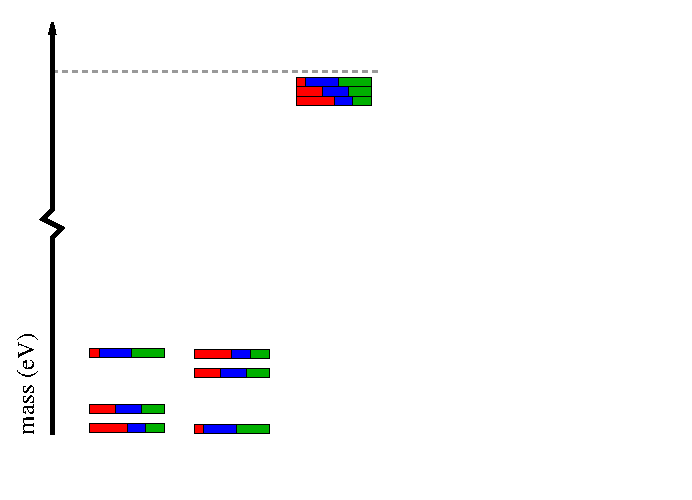
\includegraphics[height=0.8\textwidth,angle=-90]{figures/mass_scale.eps}
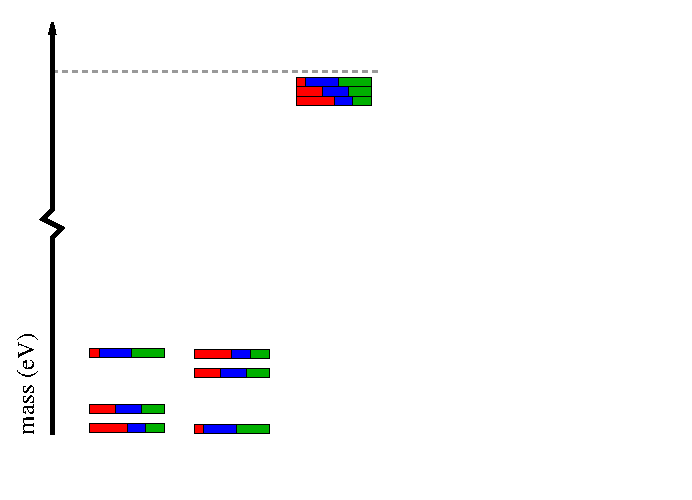
\includegraphics[width=0.8\textwidth]{figures/mass_scale.eps}
\caption[Neutrino mass hierarchies.]{The three possible mass hierarchies: normal hierarchy (NH), inverted hierarchy (IH), and quasi-degenerate (QD).  The dashed line indicates one-third the current limit for the absolute mass scale, $\sim\frac{2}{3}$~eV.}
\label{fig:massScale}
\end{figure}  

Long-baseline neutrino experiments have provided a comprehensive picture of neutrino mixing, but they cannot provide access to important information about the neutrino such as the absolute mass scale, CP-violating phases, or the origin of its small mass.  These will be discussed in the next section.


\section{Massive Neutrinos in the SM}
\label{sec:mass}
\begin{comment}
Discuss mechanisms by which neutrinos could get their mass.  
\end{comment}
In the standard model, fermions are four-component spinors that can be written in a chiral basis so that there is a ``left-handed'' component of the fermion $\psi_L$ and a ``right-handed'' component $\psi_R$, where $\psi_L$ and $\psi_R$ are two-component spinors.  The chiral basis is particularly useful because the weak bosons $W^{\pm}$ and $Z^0$ have been experimentally observed to only interact with the left-handed component of the fermion field.  The chiral basis is also helpful in understanding two possible ways to give neutrinos mass in the standard model.  Leptons acquire their mass by interacting with the Higgs field; the electron is the lightest because its coupling to the Higgs field is weaker than that of the muon.  The tau is strongly coupled to the Higgs field, making it the most massive of the leptons.  The diagram in {\fig}~\ref{fig:leptonMass} gives a heuristic picture of the lepton fields' interaction with the Higgs background.  
\begin{figure}[htp]
\centering
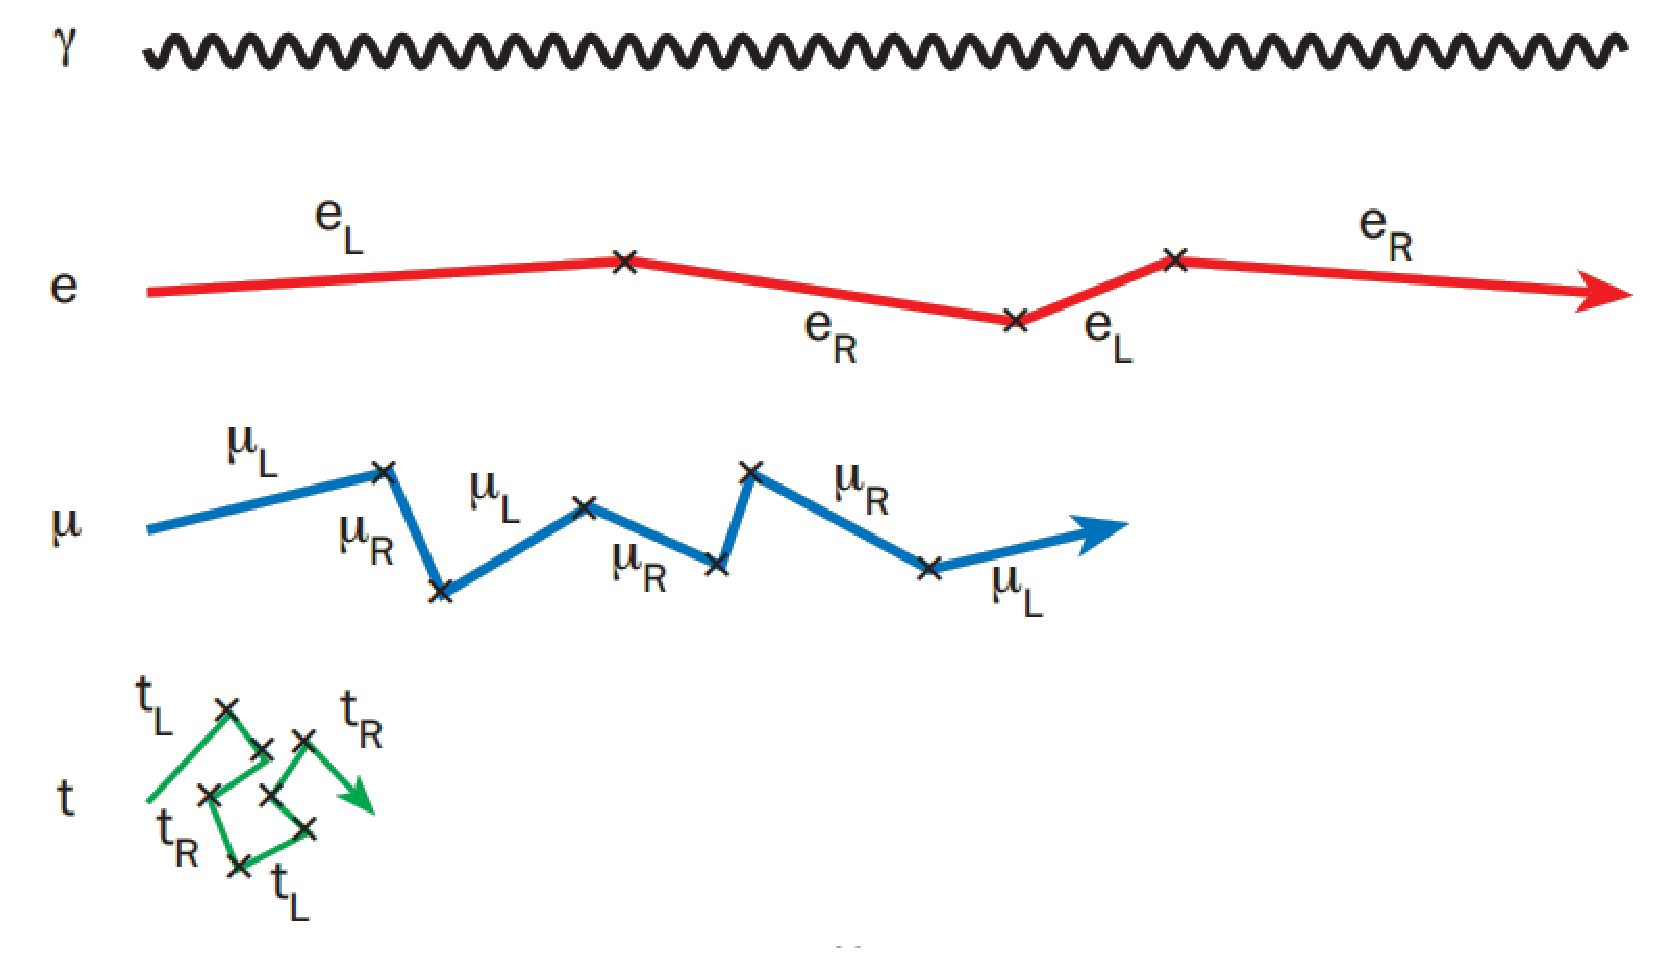
\includegraphics[width=0.8\textwidth]{figures/leptonMass.eps}
\caption[Lepton mass via the Higgs interaction.]{Leptons acquire mass by interacting with the Higgs field.  Vertices marked with $\times$ indicate an interaction with the background Higgs field.  The electron has a smaller coupling to the Higgs field than the tau and therefore interacts less.  In a Feynman diagram, lepton lines indicate already-massive leptons.  The lines here represent the  massless lepton fields and the entire diagram is analogous to a solid lepton line in a typical Feynman diagram.  Figure from {\refref}~\citep{neutrinoMass}.}
\label{fig:leptonMass}
\end{figure}
When neutrinos were thought to be massless, they were introduced into the SM as two-component spinor fields with no right-handed component.  The Higgs, which changes the chirality of the particle it interacts with, could not interact with the neutrino because it had no right-handed state to convert to.  The ansatz of a solely left-handed neutrino, then, created a massless neutrino in the SM.  As experimental evidence has overwhelmingly favored a massive neutrino, it became necessary to modify the theoretical treatment of the neutrino.  One approach is to assume that the neutrino, like the SM leptons, is a Dirac fermion and has a left-handed component as well as a right-handed component, allowing the Higgs field to interact with the neutrino as it does for the leptons.  There is another approach to generate massive neutrinos that is not solely dependent on the Higgs field.  If neutrinos are Majorana fermions, that is, if unlike Dirac fermions they are their own antiparticles, then the right-handed component of the neutrino field can introduce a mass term independent of the Higgs interaction.  When left-handed neutrinos interact with the background Higgs field, the right-handed neutrino with mass $M$ can only exist for a short time without violating the Pauli principle if $M$ is very large.  The right-handed neutrino quickly interacts with the Higgs background, transforming back into a left-handed neutrino.  The mass of the neutrino should then scaled by $m/M$, where $m$ is the mass due to interaction with the Higgs field.  See {\fig}~\ref{fig:neutrinoMass} for a picture of these different neutrino theories.  The advantage of the Majorana neutrino is that the scale of its interaction with the Higgs field can be comparable to that of other leptons; its small mass can be achieved by assuming a large $M$.  Majorana neutrinos are also attractive because a very massive neutrino could provide an explanation for the observed baryon asymmetry \citep{baryogenesis_Fukugita}.  
\begin{figure}[htp]
\centering
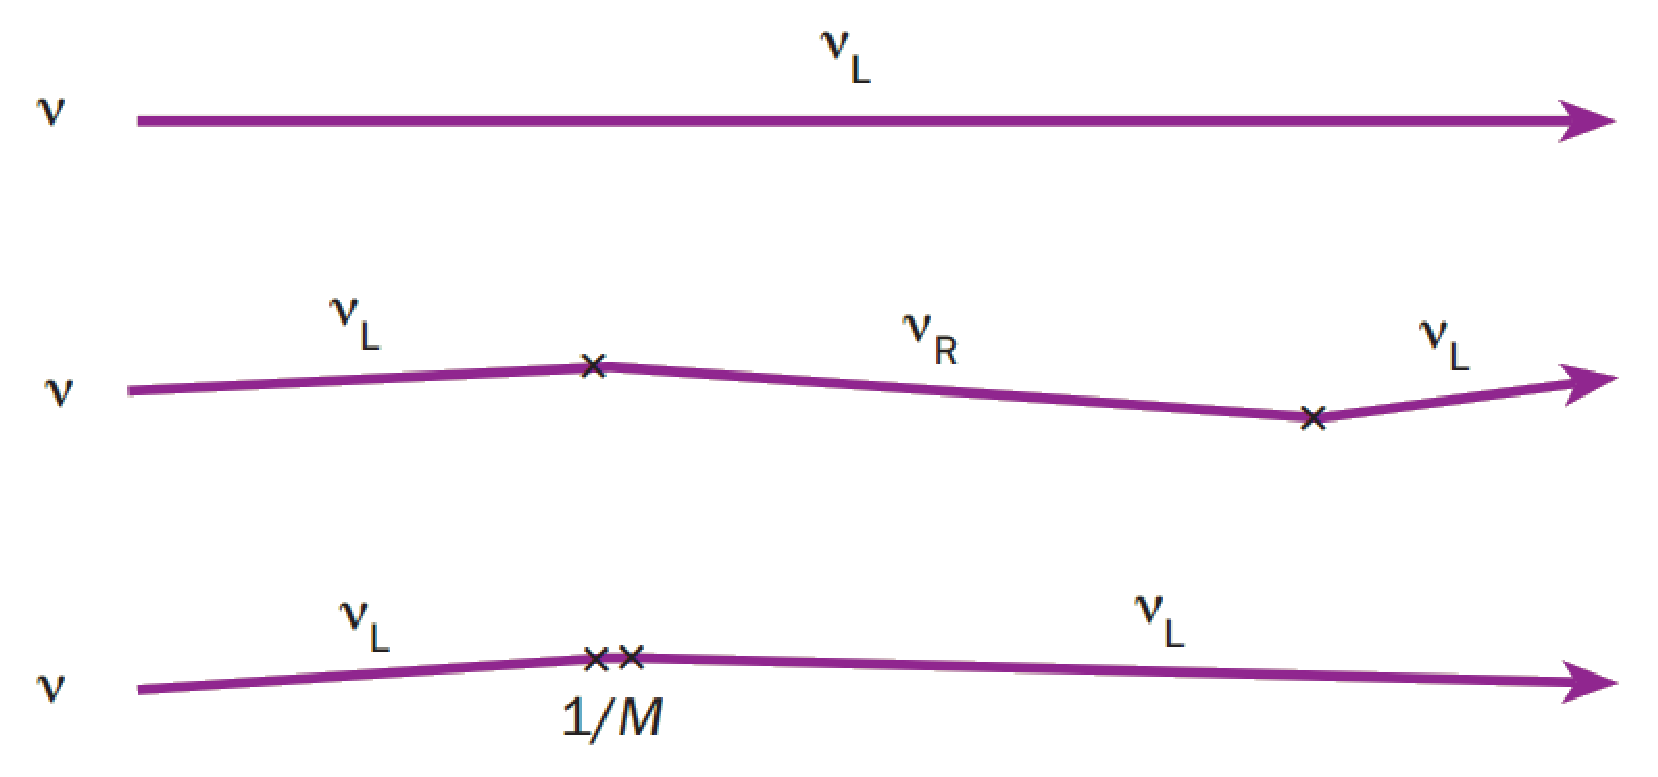
\includegraphics[width=0.8\textwidth]{figures/neutrinoMass.eps}
\caption[A depiction of massless, Dirac, and Majorana models of the neutrino.]{A representation of a massless neutrino, a Dirac neutrino, and a Majorana neutrino.  Vertices marked with $\times$ indicate an interaction with the background Higgs field.  Figure from {\refref}~\citep{neutrinoMass}.}
\label{fig:neutrinoMass}
\end{figure}  

Long-baseline experiments have determined that neutrinos are massive and have measured their mass differences and mixing angles, but much of their fundamental nature is still not understood.  That they could potentially play a significant role in many areas of physics provides significant motivation to build experiments that are sensitive to these neutrino ``parameters.'' One type of experiment that is sensitive to the Dirac or Majorana nature of the neutrino is a search for a process called neutrino-less double-beta decay (\zvbb).  Two-neutrino double-beta decay (\tvbb) is a process that has been observed for a number of nuclei and is the simultaneous beta-decay of two neutrons into two protons.  If the neutrino is a Majorana fermion, it would be possible for the neutrino to become an internal line in the Feynman diagram as shown in {\fig}~\ref{fig:zvbb}.  This process would be impossible if the neutrino were not its own antiparticle; observation of \zvbb would confirm the Majorana nature of the neutrino. 
\begin{figure}[htp]
\centering
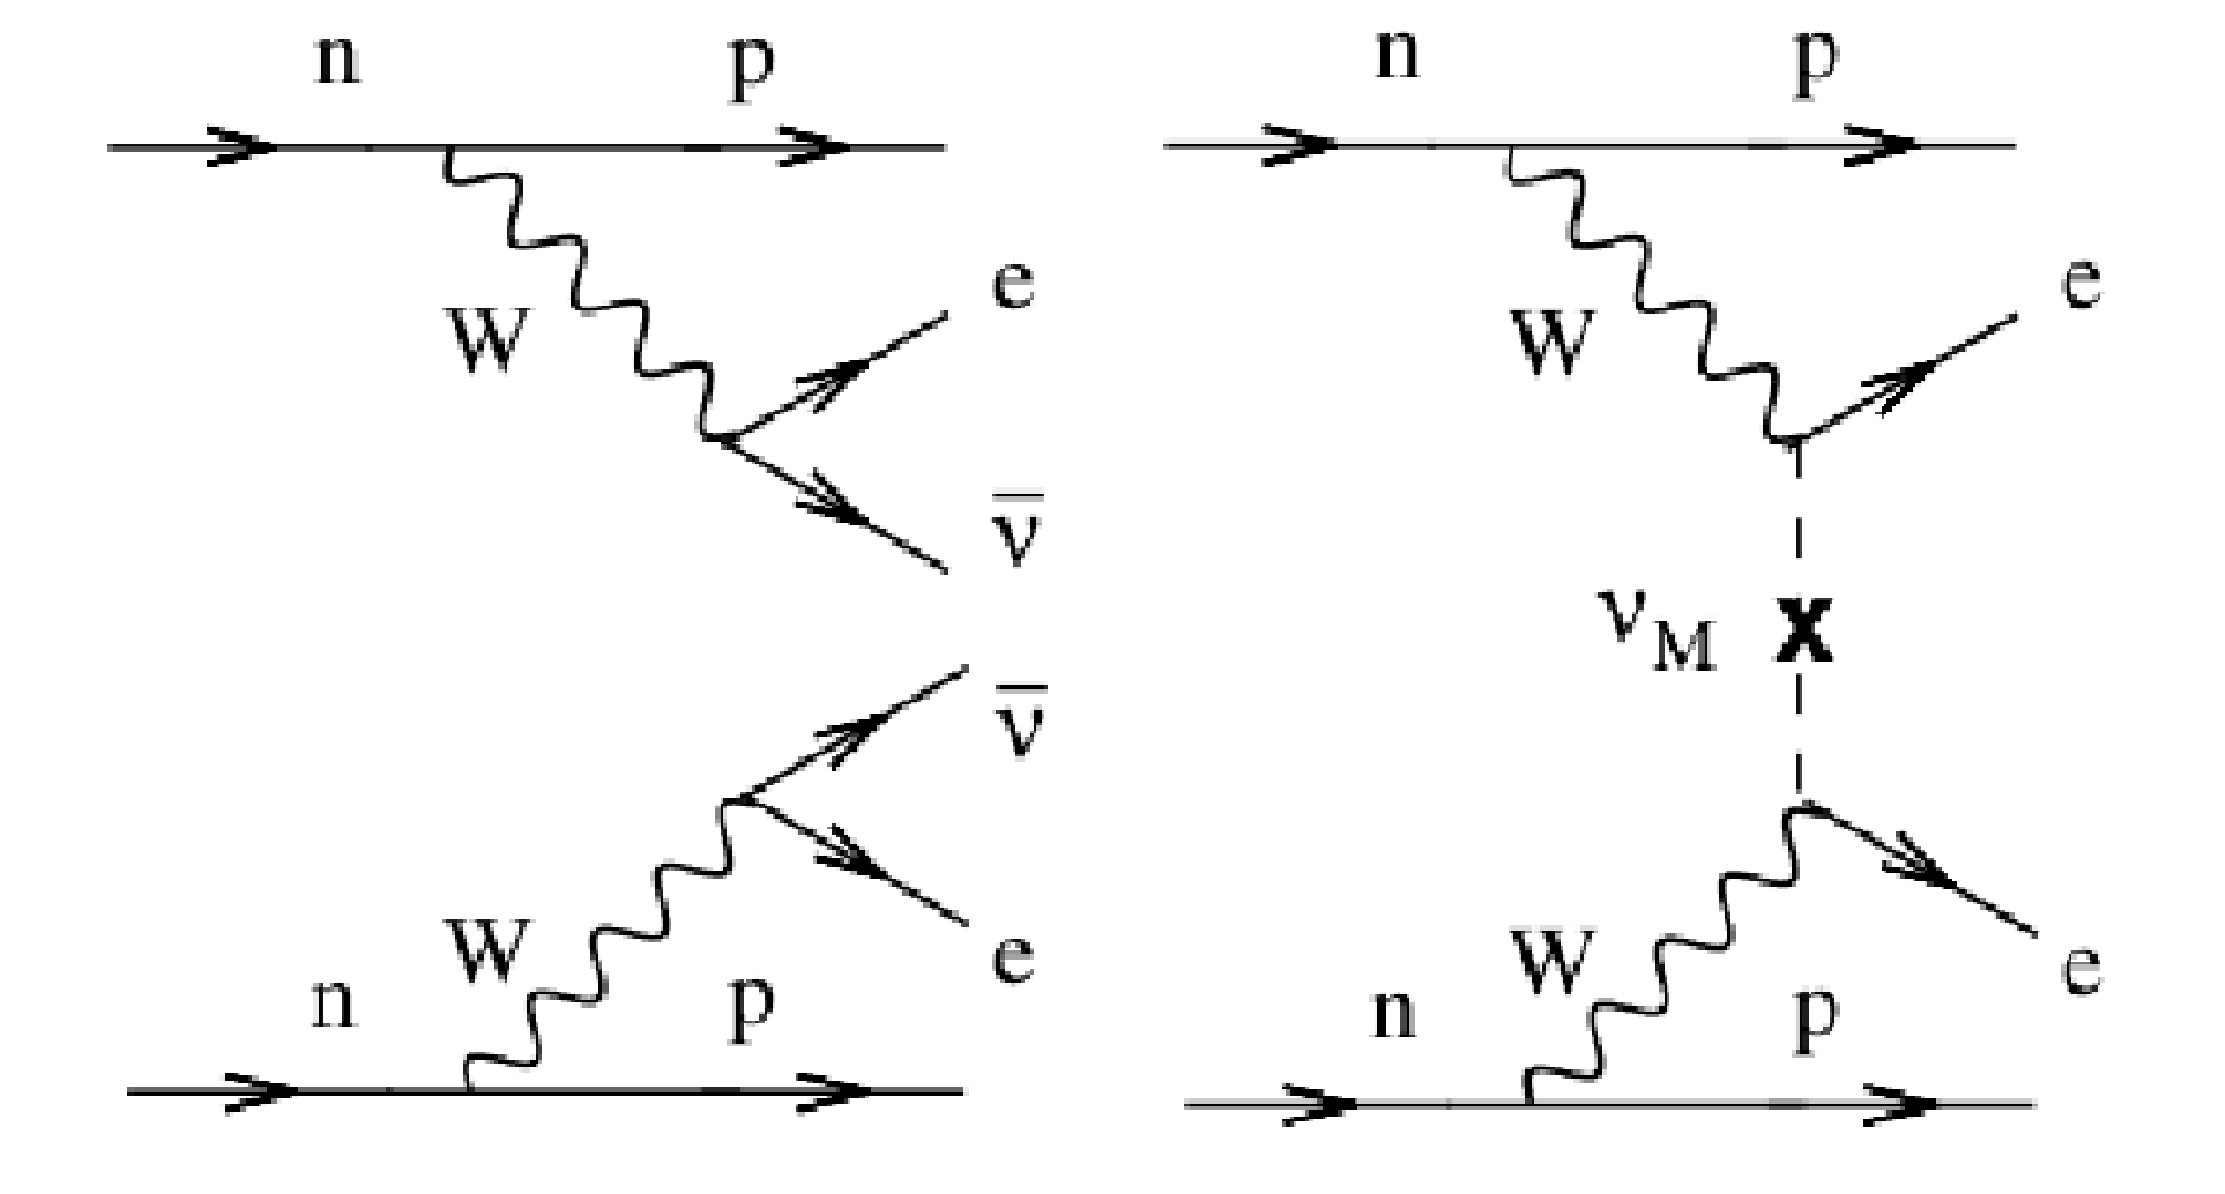
\includegraphics[width=0.8\textwidth]{figures/feynman2.eps}
\caption[Feynman diagrams describing \tvbb and \zvbb.]{Both the observed \tvbb (left) and the hypothesized \zvbb (right) modes are shown.  Nuclear matter is an ideal environment for spatially-close neutrons.  Figure from {\refref}~\citep{zvbbReview_Elliott}.}
\label{fig:zvbb}
\end{figure}
It should be noted that measured lifetimes for \tvbb are extremely long, on the order of $10^{20}$~yr.  The expected lifetime for \zvbb, if it exists, will be even larger due to the suppression of the right-handed component of the neutrino; the IGEX experiment places the current limit at $>1.57\times 10^{25}$~yr \citep{IGEX}.  This long lifetime makes \zvbb searches experimentally challenging.  However, they are currently the only way to explore crucial properties of the neutrino.  Aspects of these experiments are discussed in the next section.

\section{\zvbb searches}
\begin{comment}
Discuss \zvbb process and sensitivity to nature of neutrino.
Discuss concurrent sensitivity to hadron part
I feel like I should discuss ongoing searches but not in much detail?  Relevant information is: expected lifetime, mass, expected counts/year, expected limits?
Okay, yes.  Here is how this section could go: discuss the process and the resulting equation for the lifetime, and then talk about each of the components of the equation.  START with the discussion of the lifetime - can include details of ongoing experiments there.
\end{comment}

Searches for \zvbb are of interest not only because an observation would conclusively demonstrate that neutrinos are Majorana, but also because an observed rate gives information on the absolute mass scale of the neutrino.  The lifetime of \zvbb, assuming it results from the exchange of light Majorana neutrinos, is 
\begin{equation}
(T^{0\nu}_{1/2})^{-1} = G_{0\nu}(Q_{\beta\beta},Z)|M^{0\nu}|^2 {\langle}m_{\beta\beta}{\rangle}^2,
\end{equation}
where $G_{0\nu}(Q_{\beta\beta},Z)$ is a phase space factor, $|M^{0\nu}| = |{\langle}f|O|i{\rangle}|$, where $O$ is the \zvbb operator, is the nuclear matrix element, and $\displaystyle {\langle}m_{\beta\beta}{\rangle} \equiv |\sum_{i}m_i U_{ei}^2|$ is the effective Majorana mass.  The phase space factor can be readily calculated \citep{hadron_zvbb_Suhonen}, although it should be noted that in most current calculations, a scaling factor is introduced to this term so that \NME is a dimensionless quantity \citep{scalingFactorNME}.  The mass term is the effective mass of the electron neutrino and, unlike long-baseline experiments, is sensitive to the mass scale of the lightest neutrino particle.  This dependence is shown in {\fig}~\ref{fig:effectiveMajoranaMass} for the three possible hierarchy schemes.  
\begin{figure}[htp]
\centering
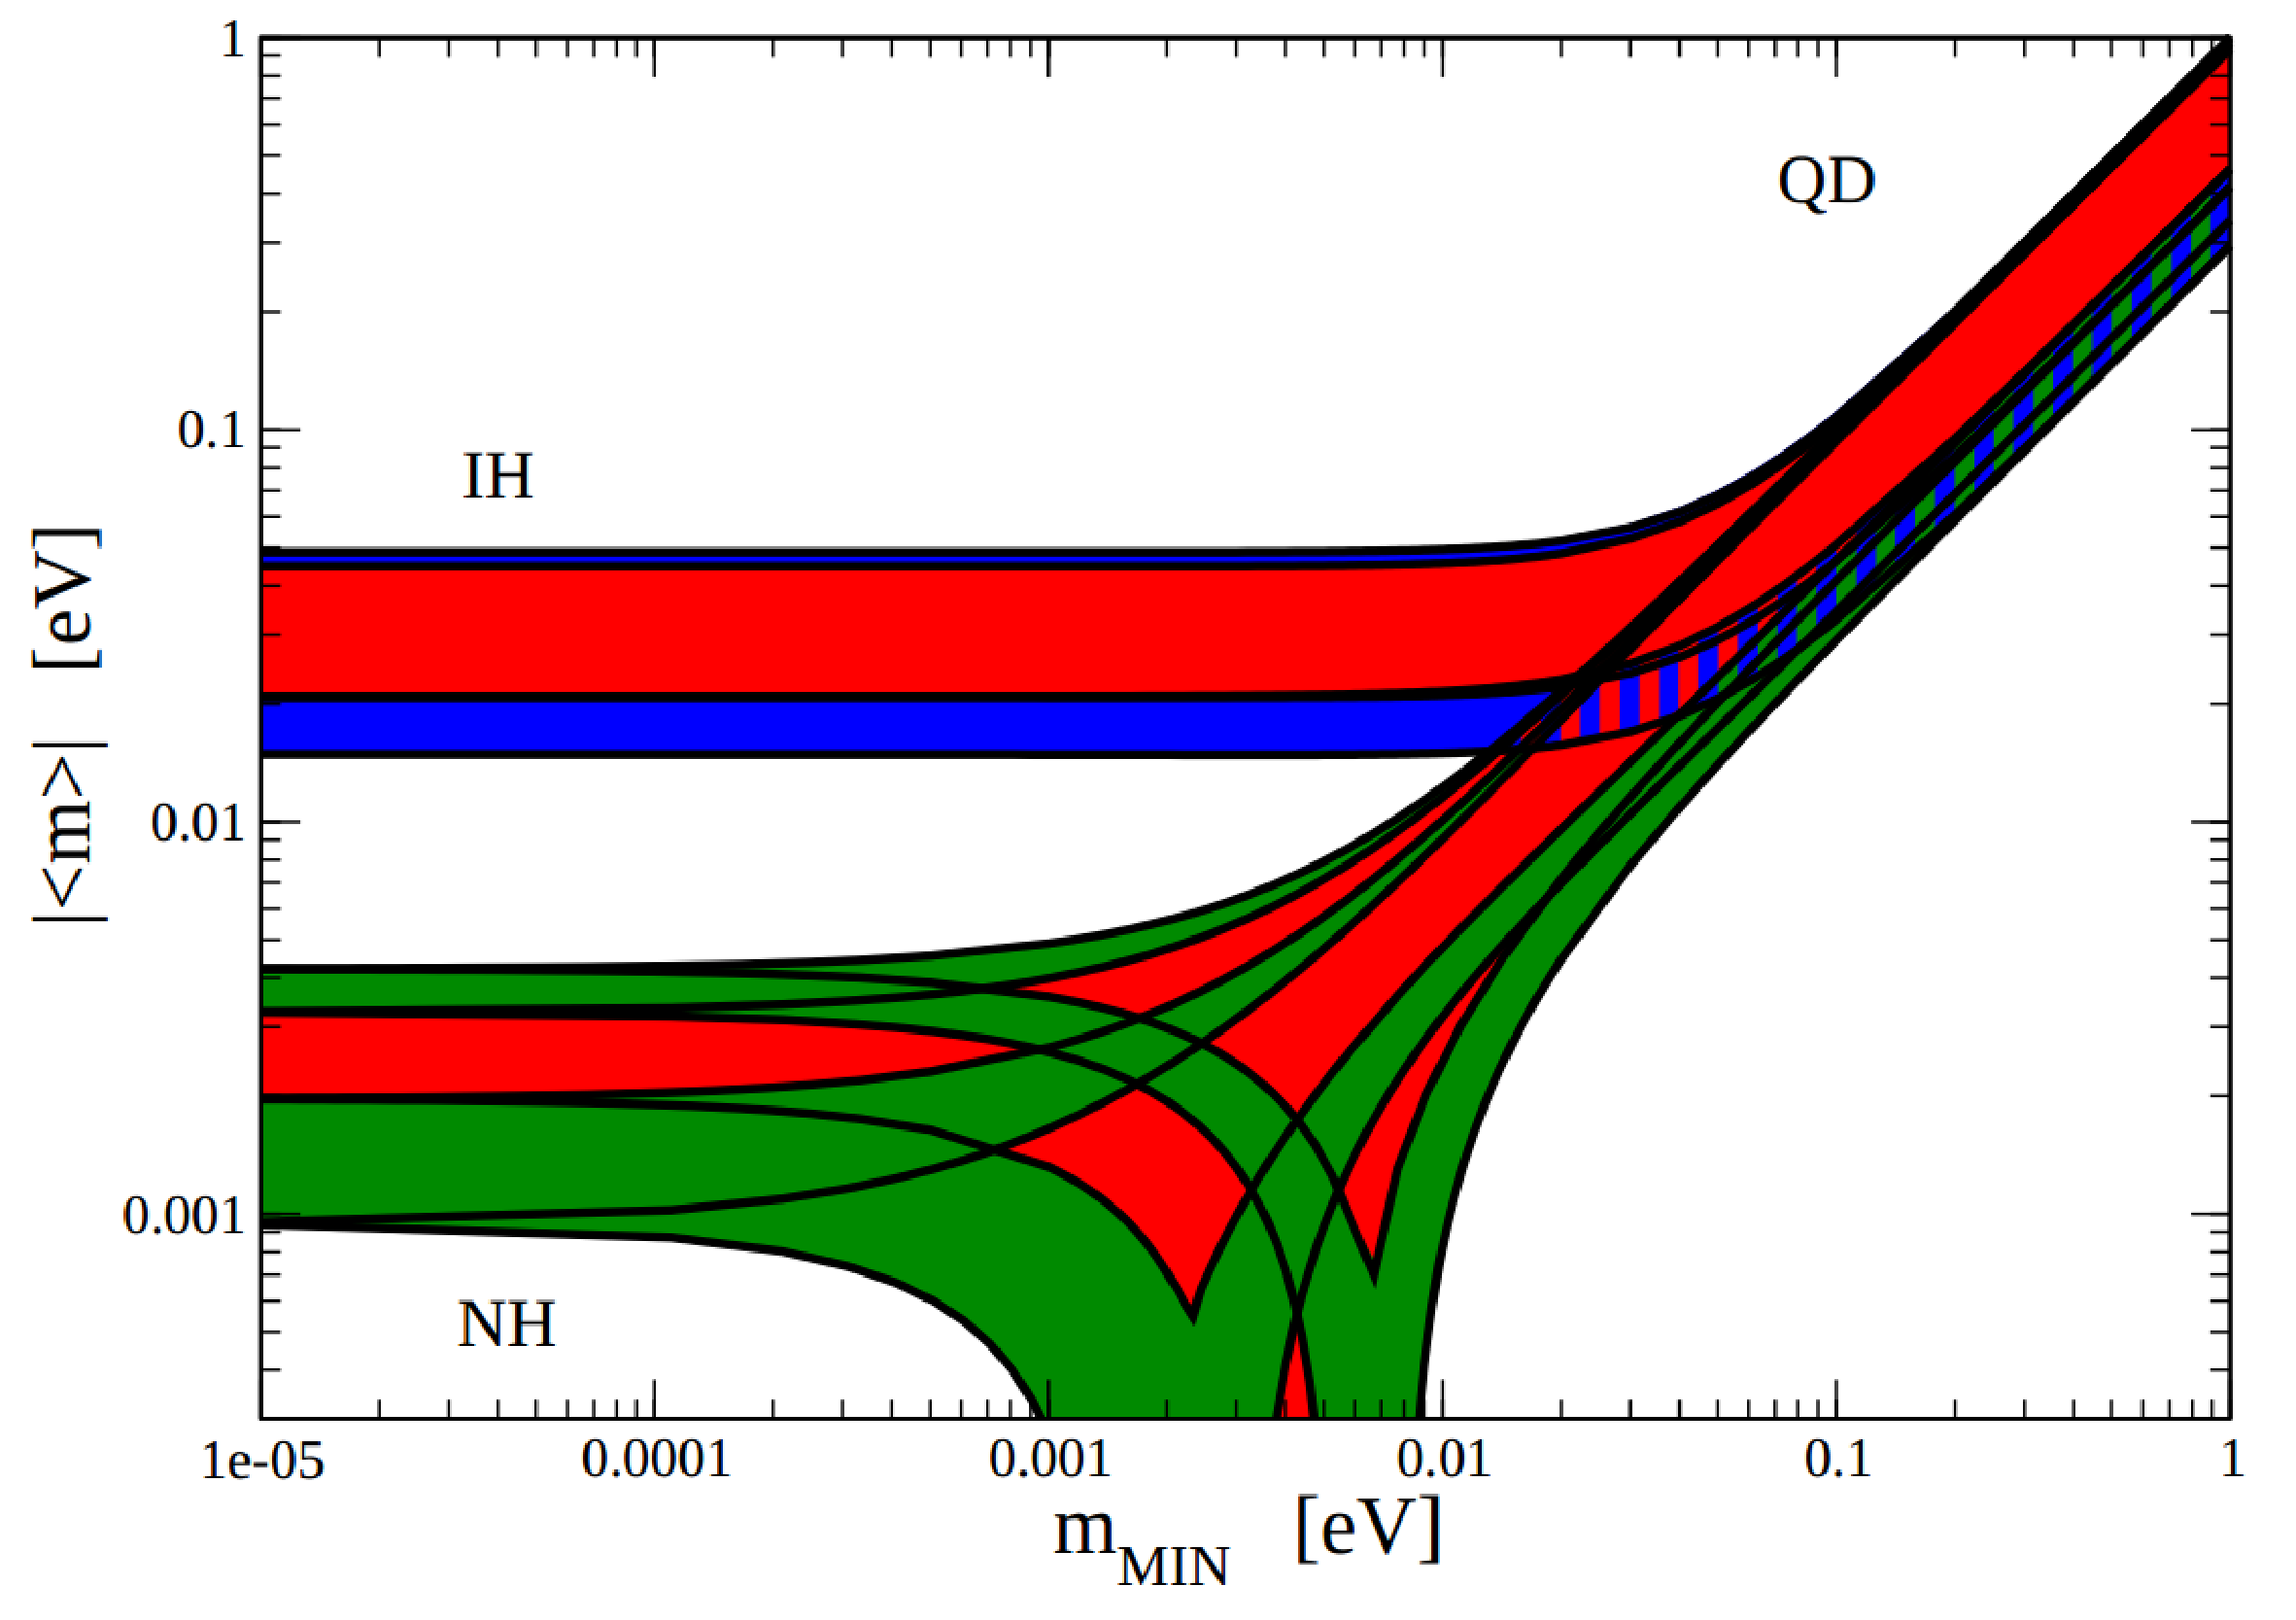
\includegraphics[width=0.8\textwidth]{figures/effectiveMajoranaMass.eps}
\caption[The effective Majorana mass as a function of the smallest neutrino mass.]{The effective Majorana mass as a function of the smallest neutrino mass $m_{min}$ for the inverse hierarchy (IH), normal hierarchy (NH), and quasi-degenerate (QD) scheme.  The values are shown in bands indicating the $2\sigma$ uncertainty.  For all values, it is assumed that $\sin^2{\theta}_{13} = 0.0236$ and $\delta = 0$.  Colors distinguish between different CP-violating scenarios of the Majorana phases.  Red bands require that $\alpha_{31}-\alpha_{21}$ as well as either $\alpha_{21}$ or $\alpha_{31}$ have a CP-violating phases.  Blue and green bands require that both $\alpha_{21}$ and $\alpha_{31}$ have CP-conserving phases.  Overlapping regions are shown hatched.  Figure from {\refref}~\citep{PDG}.}
\label{fig:effectiveMajoranaMass}
\end{figure}

The hadronic dependence of the lifetime, \NME, is sensitive to the initial and final nuclear wavefunctions.  Details of these calculations are discussed in {\chap}~\ref{chap:nucl}, but it should be noted that calculated \NME values for most candidate nuclei vary by as much as a factor of 5.
\begin{figure}[htp]
\centering
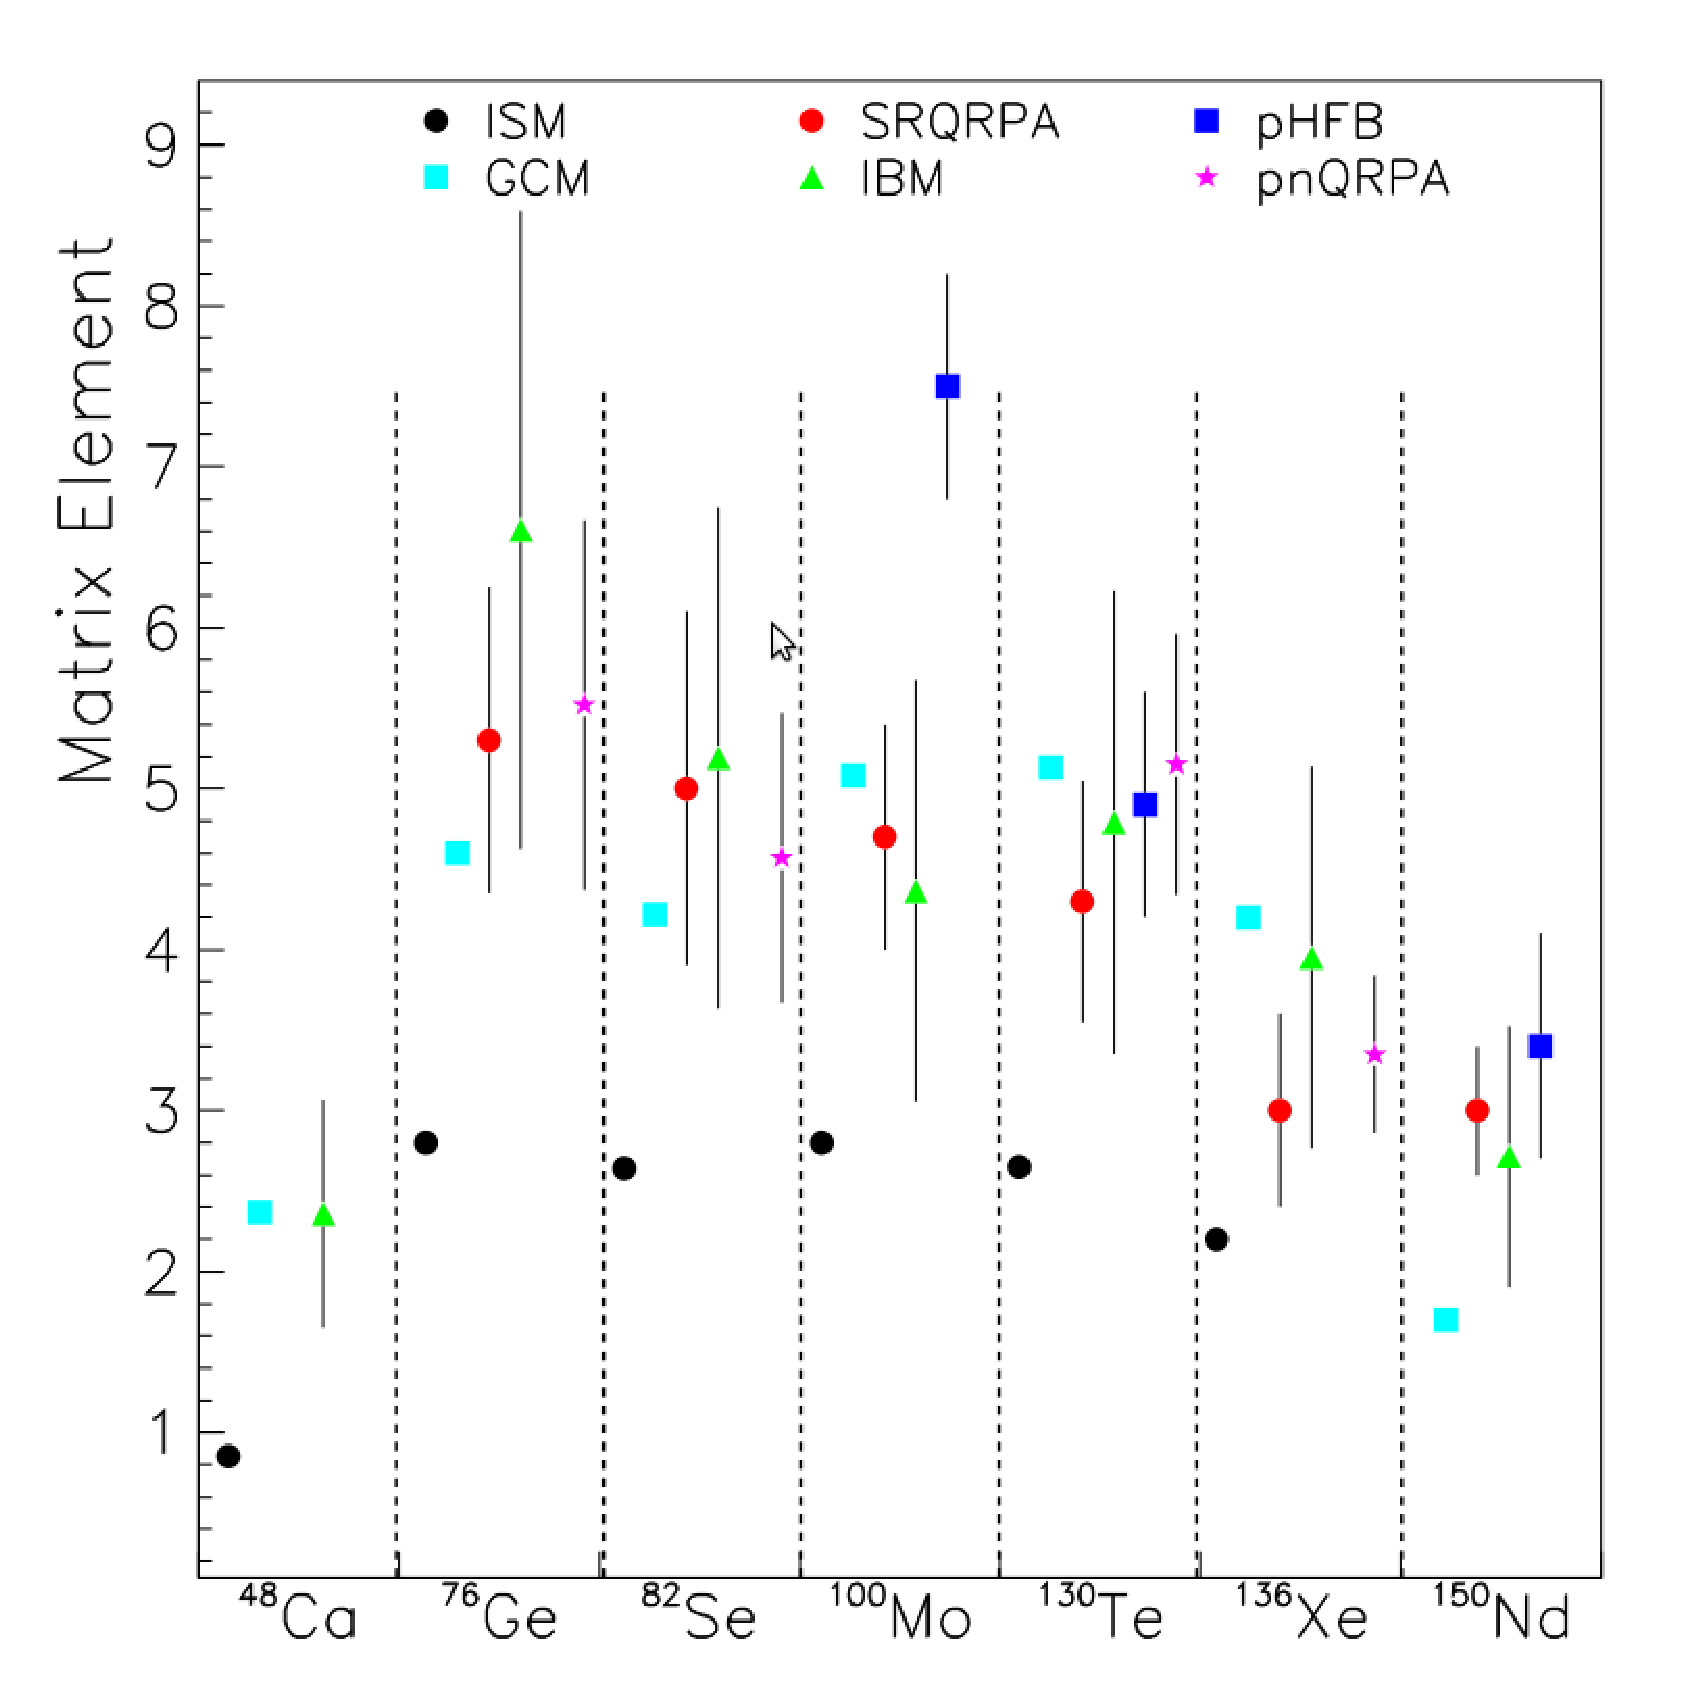
\includegraphics[width=0.8\textwidth]{figures/differentNME.eps}
\caption[Uncertainty in current calculated values of \NME.]{Calculated \NME for candidate \zvbb nuclei.  The models used for these calculations are the Interacting Shell Model (ISM) \citep{ISM}, self-consistent renormalized quasi-particle random phase approximation (SRQRPA) \citep{FaesslerReview}, proton-neutron quasi-particle random phase approximation (PNQRPA) \citep{pnQRPA_Suhonen}, generating coordinate method (GCM) \citep{GCM}, the interacting boson model (IBM) \citep{IBM_Iachello}, and the projected Hartree-Fock-Bogoliubov (pHFB) \citep{pHFB}.  Figure taken from \citep{zvbbReviewSchwingenheuer}.  Note that \NME is a dimensionless quantity; this is accomplished by multiplying by the nuclear radius, typically chosen to be $1.2A^{1/3}$~fm.  For details on the use of this factor in \NME calculations see {\ref}~\citep{scalingFactorNME}.}
\label{fig:differentNME}
\end{figure}  
This uncertainty in \NME directly affects the limits that can be placed on the neutrino mass scale if \zvbb is observed.  Transfer reactions, discussed in {\chap}~\ref{chap:nucl}, offer valuable experimental data that can be used to understand which models are most appropriate for these nuclei and improve the accuracy of the calculations.  The topic of this thesis is the two-proton transfer reaction, which is also discussed in {\chap}~\ref{chap:nucl}.

Nuclei that are suitable for \zvbb experiments are those that are stable against single beta decay but energetically allowed to double-beta decay.  This is the same group of nuclei in which \tvbb has been studied.  The \zvbb peak is at the endpoint of the \tvbb spectrum, and in fact the \tvbb process is a significant background to \zvbb due to finite detector resolution.  The nuclei $^{48}$Ca, \Ge{76}, \Se{82}, $^{100}$Mo, $^{130}$Te, $^{136}$Xe, and $^{150}$Nd have been used to search for the process in past and present experiments.  See {\tab}~\ref{tab:experiments} for a list of past and present experiments.  Because of the uncertainties on \NME for these nuclei (see {\fig}~\ref{fig:differentNME}, it is not clear which, if any, would enjoy a shorter $T^{0\nu}_{1/2}$.  So many different experiments have arisen because each candidate nucleus offers different advantages in experimental design.  \Ge{76} is an appealing candidate because the active volume also serves as the detector, and Ge crystals are well understood.  Experiments using \Ge{76} are also important because the Heidelberg-Moscow experiment, which claimed an observed \zvbb signal \citep{KlapdorKleingrothaus}, used \Ge{76} crystals.  Other nuclei are appealing because they have high abundance or are easy to obtain.  This is the case for $^{136}$Xe, which is currently being used by the EXO-200 collaboration \citep{EXO200}.  Experiments using $^{136}$Xe typically use time projection chambers (TPC's), which are able to strongly reduce background by reconstructing the momenta of particles in a decay.  Using $^{136}$Xe is particularly appealing because large quantities are readily available, reducing the cost of increasing the mass scale of the experiment.  Another candidate nucleus, $^{130}$Te, is frequently used in experiments using bolometry to detect \zvbb.  A summary of \zvbb searches is shown in {\tab}~\ref{tab:experiments}.
\begin{sidewaystable}
\ra{1.1}\small
\centering
\caption[\zvbb \uppercase{experiments}]{\\\zvbb \uppercase{experiments}}
\label{tab:experiments}

\begin{tabular}{@{}rlllllll@{}}\toprule
\multicolumn{1}{l}{Experiment} & Isotope & Mass [kg] & Method & $T^{2\nu}_{1/2}$ [yr] & $T^{0\nu}_{1/2}$ [yr] & Start - End & {\refref} \\
\midrule
\multicolumn{1}{l}{\textbf{Past Experiments}} \\
Heidelberg-Moscow & \Ge{76} & 11 & ionization & $(1.74\pm0.18)\times 10^{21}$ & $1.19^{+2.99}_{-0.5}\times 10^{25}$ &1990 - 2003 & \citep{KlapdorKleingrothaus} \\
Cuorcino & $^{130}$Te & 11 & bolometer & & $> 2.8\times 10^{24}$ & 2003 - 2008 & \citep{Cuorcino} \\
NEMO-3 & $^{100}$Mo & 7 & track + calorim. & $(0.716\pm0.055)\times 10^{19}$ & $> 1.0\times 10^{24}$ & 2003 - 2009 & \citep{NEMO3} \\
NEMO-3 & $^{82}$Se & 1 & track + calorim. & $(9.6\pm1.1)\times 10^{19}$ & $> 3.2\times 10^{23}$ & 2003 - 2009 & \citep{NEMO3} \\
\noalign{\vskip 0.3cm}

\multicolumn{1}{l}{\textbf{Current Experiments}} \\
EXO-200 & $^{136}$Xe & 175 & liquid TPC & $(2.1\pm0.2)\times 10^{21}$ & $>1.6\times 10^{25}$ & 2011 - & \citep{EXO200} \\
Kamland-Zen & $^{136}$Xe & 330 & liquid scint. & $(2.38\pm0.14)\times 10^{21}$ & $>5.7\times 10^{24}$ & 2011 - & \citep{KamLAND_Zen} \\
GERDA-I/GERDA-II & \Ge{76} & 15/35 & ionization & $(1.88\pm0.1)\times 10^{21}$ & & 2011/2013 - & \citep{Gerda} \\
CANDLES & $^{48}$Ca & 0.35 & scint. crystal & & & 2011 - & \citep{CANDLES} \\
\noalign{\vskip 0.3cm}

\multicolumn{1}{l}{\textbf{Funded Experiments}} \\
NEXT & $^{136}$Xe & 100 & gas TPC & & & 2015 - & \citep{NEXT} \\
Cuore0/Cuore & $^{130}$Te & 10/200 & bolometer & & & 2012/2015 - & \citep{Cuore} \\
Majorana Demo & \Ge{76} & 30 & ionization & & & 2013 - & \citep{Majorana} \\
SuperNEMO Demo & \Se{82} & 7 & track + calorim. & & & 2014 - & \citep{SuperNEMO} \\
SNO+ & $^{150}$Nd & 44 & liquid scint. & & & 2013 - & \citep{SNO} \\
\bottomrule
\end{tabular}
\begin{flushleft}
\small NOTE:
Past, present, and future \zvbb experiments.  Detecting a signal in several different isotopes would greatly improve the likelihood of a Majorana process.  From \citep{zvbbReviewSchwingenheuer}.
\end{flushleft}
\end{sidewaystable}

Searches for \zvbb offer access to unique areas of neutrino physics.  Confirmation of the process would demonstrate that neutrinos are Majorana in nature and would also provide a measurement of the absolute mass scale of the electron neutrino.  The dependence of the lifetime on \NME poses a difficulty because the current uncertainty in calculations limits the sensitivity to the neutrino mass scale and also increases the difficulty of planning experiments that search for the process.  Nuclear transfer experiments provide information that can help reduce the uncertainty of \NME calculations, and this thesis focuses on two-proton transfers in the Ge nuclei.  The impact of such a transfer experiment is discussed in {\chap}~\ref{chap:nucl}.


% % uncomment the following lines,
% if using chapter-wise bibliography
%
% \bibliographystyle{ndnatbib}
% \bibliography{example}



%
% Chapter 2
%

%
% Modified by Sameer Vijay
% Last Change: Wed Jul 27 2005 13:00 CEST
%
%%%%%%%%%%%%%%%%%%%%%%%%%%%%%%%%%%%%%%%%%%%%%%%%%%%%%%%%%%%%%%%%%%%%%%%%
%
% Sample Notre Dame Thesis/Dissertation
% Using Donald Peterson's ndthesis classfile
%
% Written by Jeff Squyres and Don Peterson
%
% Provided by the Information Technology Committee of
%   the Graduate Student Union
%   http://www.gsu.nd.edu/
%
% Nothing in this document is serious except the format.  :-)
%
% If you have any suggestions, comments, questions, please send e-mail
% to: ndthesis@gsu.nd.edu
%
%%%%%%%%%%%%%%%%%%%%%%%%%%%%%%%%%%%%%%%%%%%%%%%%%%%%%%%%%%%%%%%%%%%%%%%%

%
% Chapter 2
%

\chapter{TRANSFER REACTIONS AND NUCLEAR MATRIX ELEMENTS}
\label{chap:nucl}

The nuclear matrix elements for the \tvbb process are well-understood, but calculation of \NME for the \zvbb process is significantly different \citep{VogelReview}.  This chapter discusses the calculation of \NME for the \zvbb process and the constraints that can be placed on these calculations with experimental data, including the two-proton transfer data that is the topic of this thesis.  The shell model of the nucleus underlies all further discussions of \NME and interpretation of experimental results and is discussed first.    

\section{Shell Model of the Nucleus}
\begin{comment}
Using H.O. eigenstates to describe nucleons.
\begin{itemize}
\item nuclear potential well - is this something we can understand independently?  Certainly the radius is.
\item solutions to finite square well in terms of H.O. eigenstates and a diagram of energy levels
\item the energy levels give correct shell closures when spin-orbit coupling is introduced
\item so H.O. eigenstates are a reasonable way to describe nucleons
\end{itemize}

Looking at the valence nucleons to understand the whole nucleus.
\begin{itemize}
\item and because the nucleons couple so strongly into \zp pairs, describing the unpaired nucleons often accurately describes the entire nucleus
\item give a simple example?  \He{3} might be useful?
\item show level filling for \Ge{74} (32 protons) and point out the valence nucleons are f, p, g
\end{itemize}
\end{comment}

Trends in systematic nuclear data such as nuclear mass, proton and neutron separation energies, and the energy of the first excited state give clear evidence of ``magic numbers'' of protons and neutrons in nuclei.  {\fig}~\ref{fig:alphaSep} shows the alpha separation energy with increasing neutron number $N$, which also shows this systematic behavior.  Such a structure is suggestive of that seen in atomic electrons, which experience a central potential primarily due to the Coulomb interaction.  However, the Coulomb potential is not an appropriate model for nuclei, where the potential is known to be short range \citep{Casten}.  One model that has promising beginnings is the harmonic oscillator potential.  To determine the magic numbers predicted by this potential, consider the quantum numbers that describe an eigenstate of this potential.  The principal quantum number, $n$, indicates the number of nodes of the state.  In this work, the node at infinity is included rather than the node at zero, so that $n$ ranges from 1 to $\infty$.  The orbital angular momentum is denoted $l$, with $l = 0, 1, 2, 3, ...$ typically called the $s, p, d, f, ...$ orbitals as in atomic electron structure.  The eigenvalue associated with the projection of the orbital angular momentum operator along the $z$-axis is $m$, which varies between $-l$ and $l$ and is called the magnetic quantum number.  The eigenvalues of any eigenstate of a spherically symmetric potential cannot depend on the magnetic quantum number, so that for the harmonic oscillator potential, any state associated with $l$ has a multiplicity of $2(2l+1)$, where the additional factor of two is due to nucleons being spin-1/2 fermions.  The eigenvalues of the three-dimensional harmonic oscillator are $E_{nl} = (2n+l-\frac{1}{2})\hbar\omega$, so that the energies proceed in uniform steps as $2n+l$ increases by one unit.  {\fig}~\ref{fig:shellModelMagic} shows the level spacing for this potential; note that the energy levels are multiplets.  For example, the states $nl = 2s$ and $1d$ both have energy $\frac{3}{2}\hbar\omega$.  

\begin{figure}[hp]
\centering
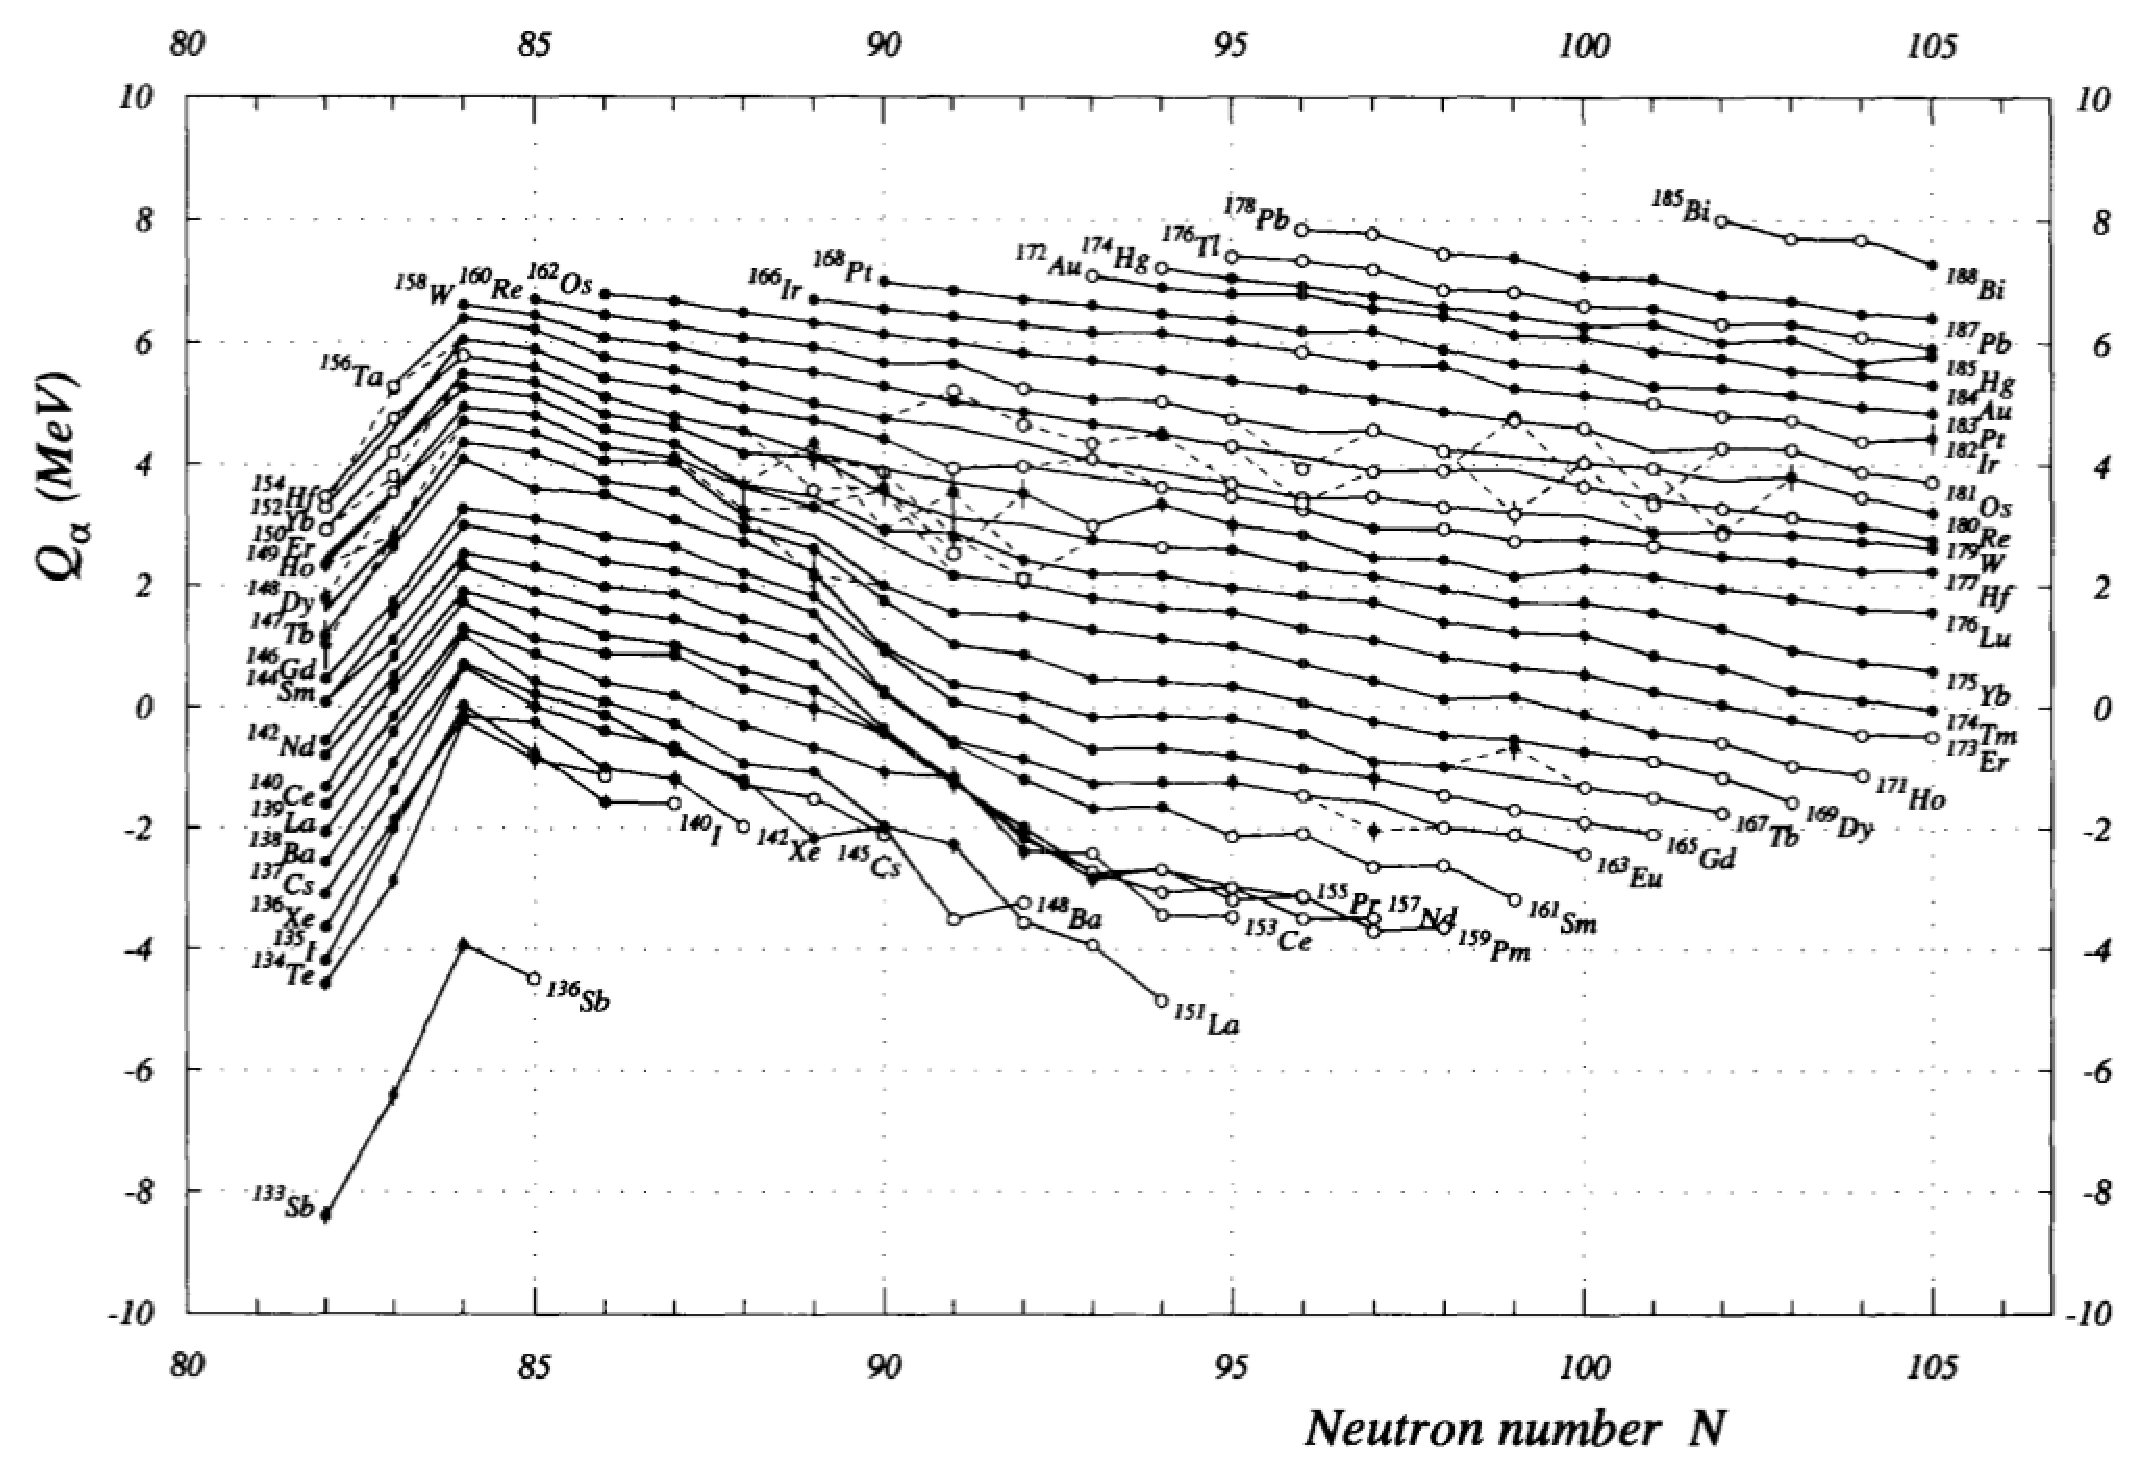
\includegraphics[width=0.8\textwidth]{figures/alphaSepEnergy.eps}
\caption[Alpha separation energy as an illustration of shell structure.]{Alpha separation energy as a function of neutron number.  The behavior around $N=84$ is indicative of shell structure.  From {\refref}~\citep{massEval_1993}.}
\label{fig:alphaSep}
\end{figure}
% another float
\begin{figure}[hp]
\centering
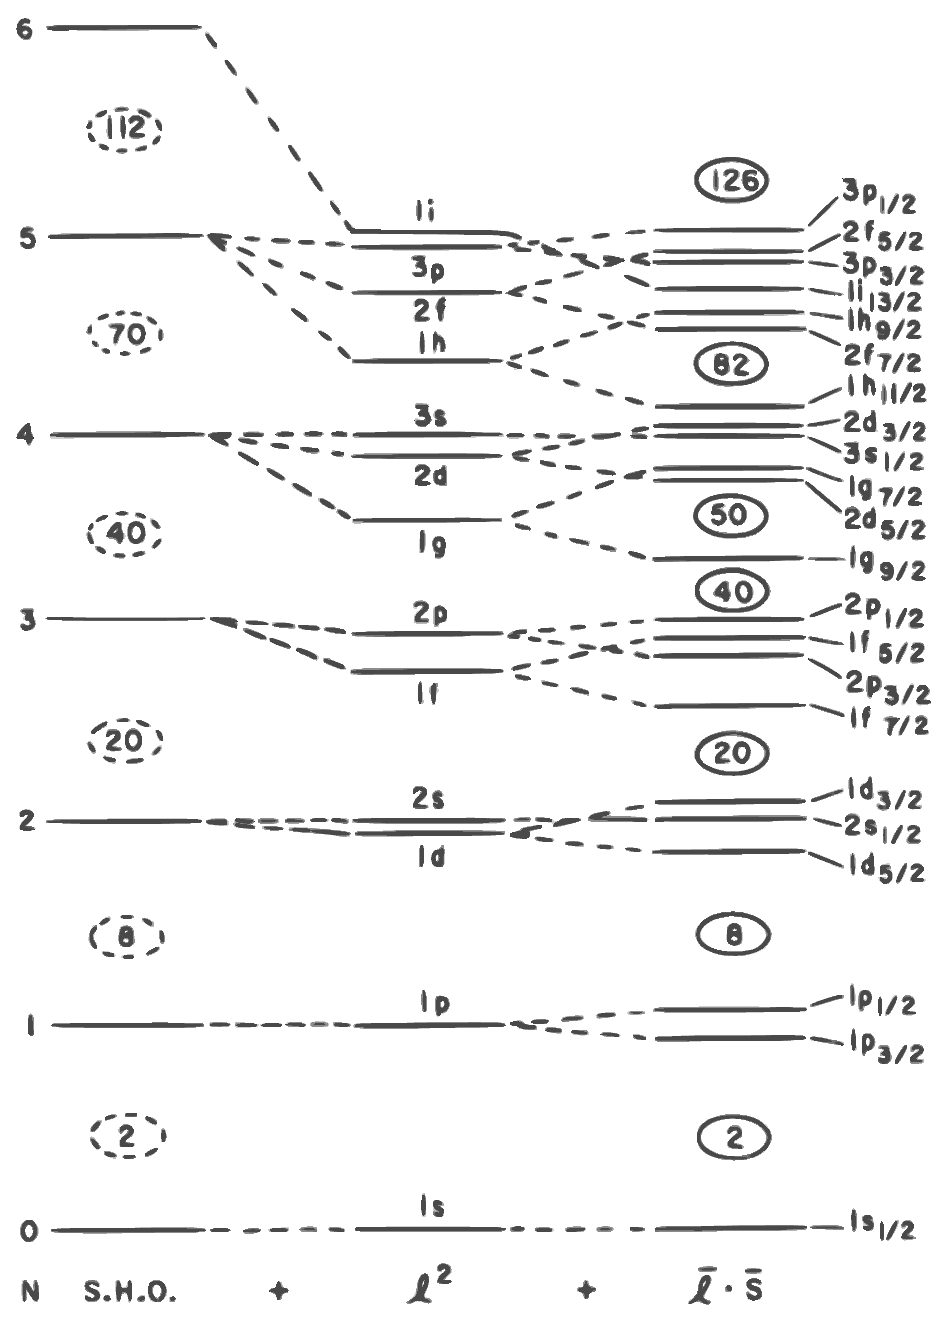
\includegraphics[width=0.8\textwidth]{figures/nuclearLevels.eps}
\caption[Level diagrams for different models of the nuclear Hamiltonian.]{Level diagrams for different models of the nuclear potential and their predicted magic numbers.  From left to right are the simple harmonic oscillator, a more flat-bottomed potential resulting from adding an $l^2$ term, and finally the addition of the spin-orbit coupling.  From {\refref}~\citep{Casten}.}
\label{fig:shellModelMagic}
\end{figure}

The harmonic oscillator potential predicts magic numbers at 2, 8, 20, 40, 70, and 112.  This matches the observed pattern for low numbers but begins to deviate for heavier nuclei.  A reasonable correction to make to the potential is to make it more uniform to more accurately reflect the fact that the density of nuclei is quite uniform \citep{Casten}.  Introducing a potential term proportional to $l^2$ does this by reducing the potential near the center of the well (where the orbital angular momentum is smaller) and increasing the potential further from the center, where the orbital angular momentum is larger.  Adjusting the potential in this way splits the $l$-degeneracy of the states but does not fundamentally change the predicted magic numbers.  It was not until Maria Goeppert-Mayer added a spin-orbit term to the potential \citep{MGM} that these magic numbers were correctly reproduced.  

Although the harmonic oscillator potential is useful in understanding many aspects of nuclear structure with the benefit of having well-understood quantum numbers, it has a number of shortcomings.  One has already been discussed - the bottom of the potential should be flatter to better describe the uniformity of nuclear matter.  This can be corrected by adding an $l^2$ term to the harmonic oscillator, but another approach is to define a new potential.  The Woods-Saxon potential \citep{WoodsSaxon} shown in {\fig}~\ref{fig:woodsSaxon} is a potential that reflects many of the known physical features of the nuclear potential and has the same quantum numbers as the modified harmonic oscillator potential described above.  The functional form of the Woods-Saxon potential is 
\begin{equation}
V(r) = \frac{V}{1+e^{(r-r_0)/a}},
\end{equation}
where $r$ is the distance from the center and the constants $V$, $r_0$, and $a$ represent the depth of the potential, the characteristic radius, and the surface diffusivity.  All further calculations discussed in this use this potential.
\begin{figure}[hp]
\centering
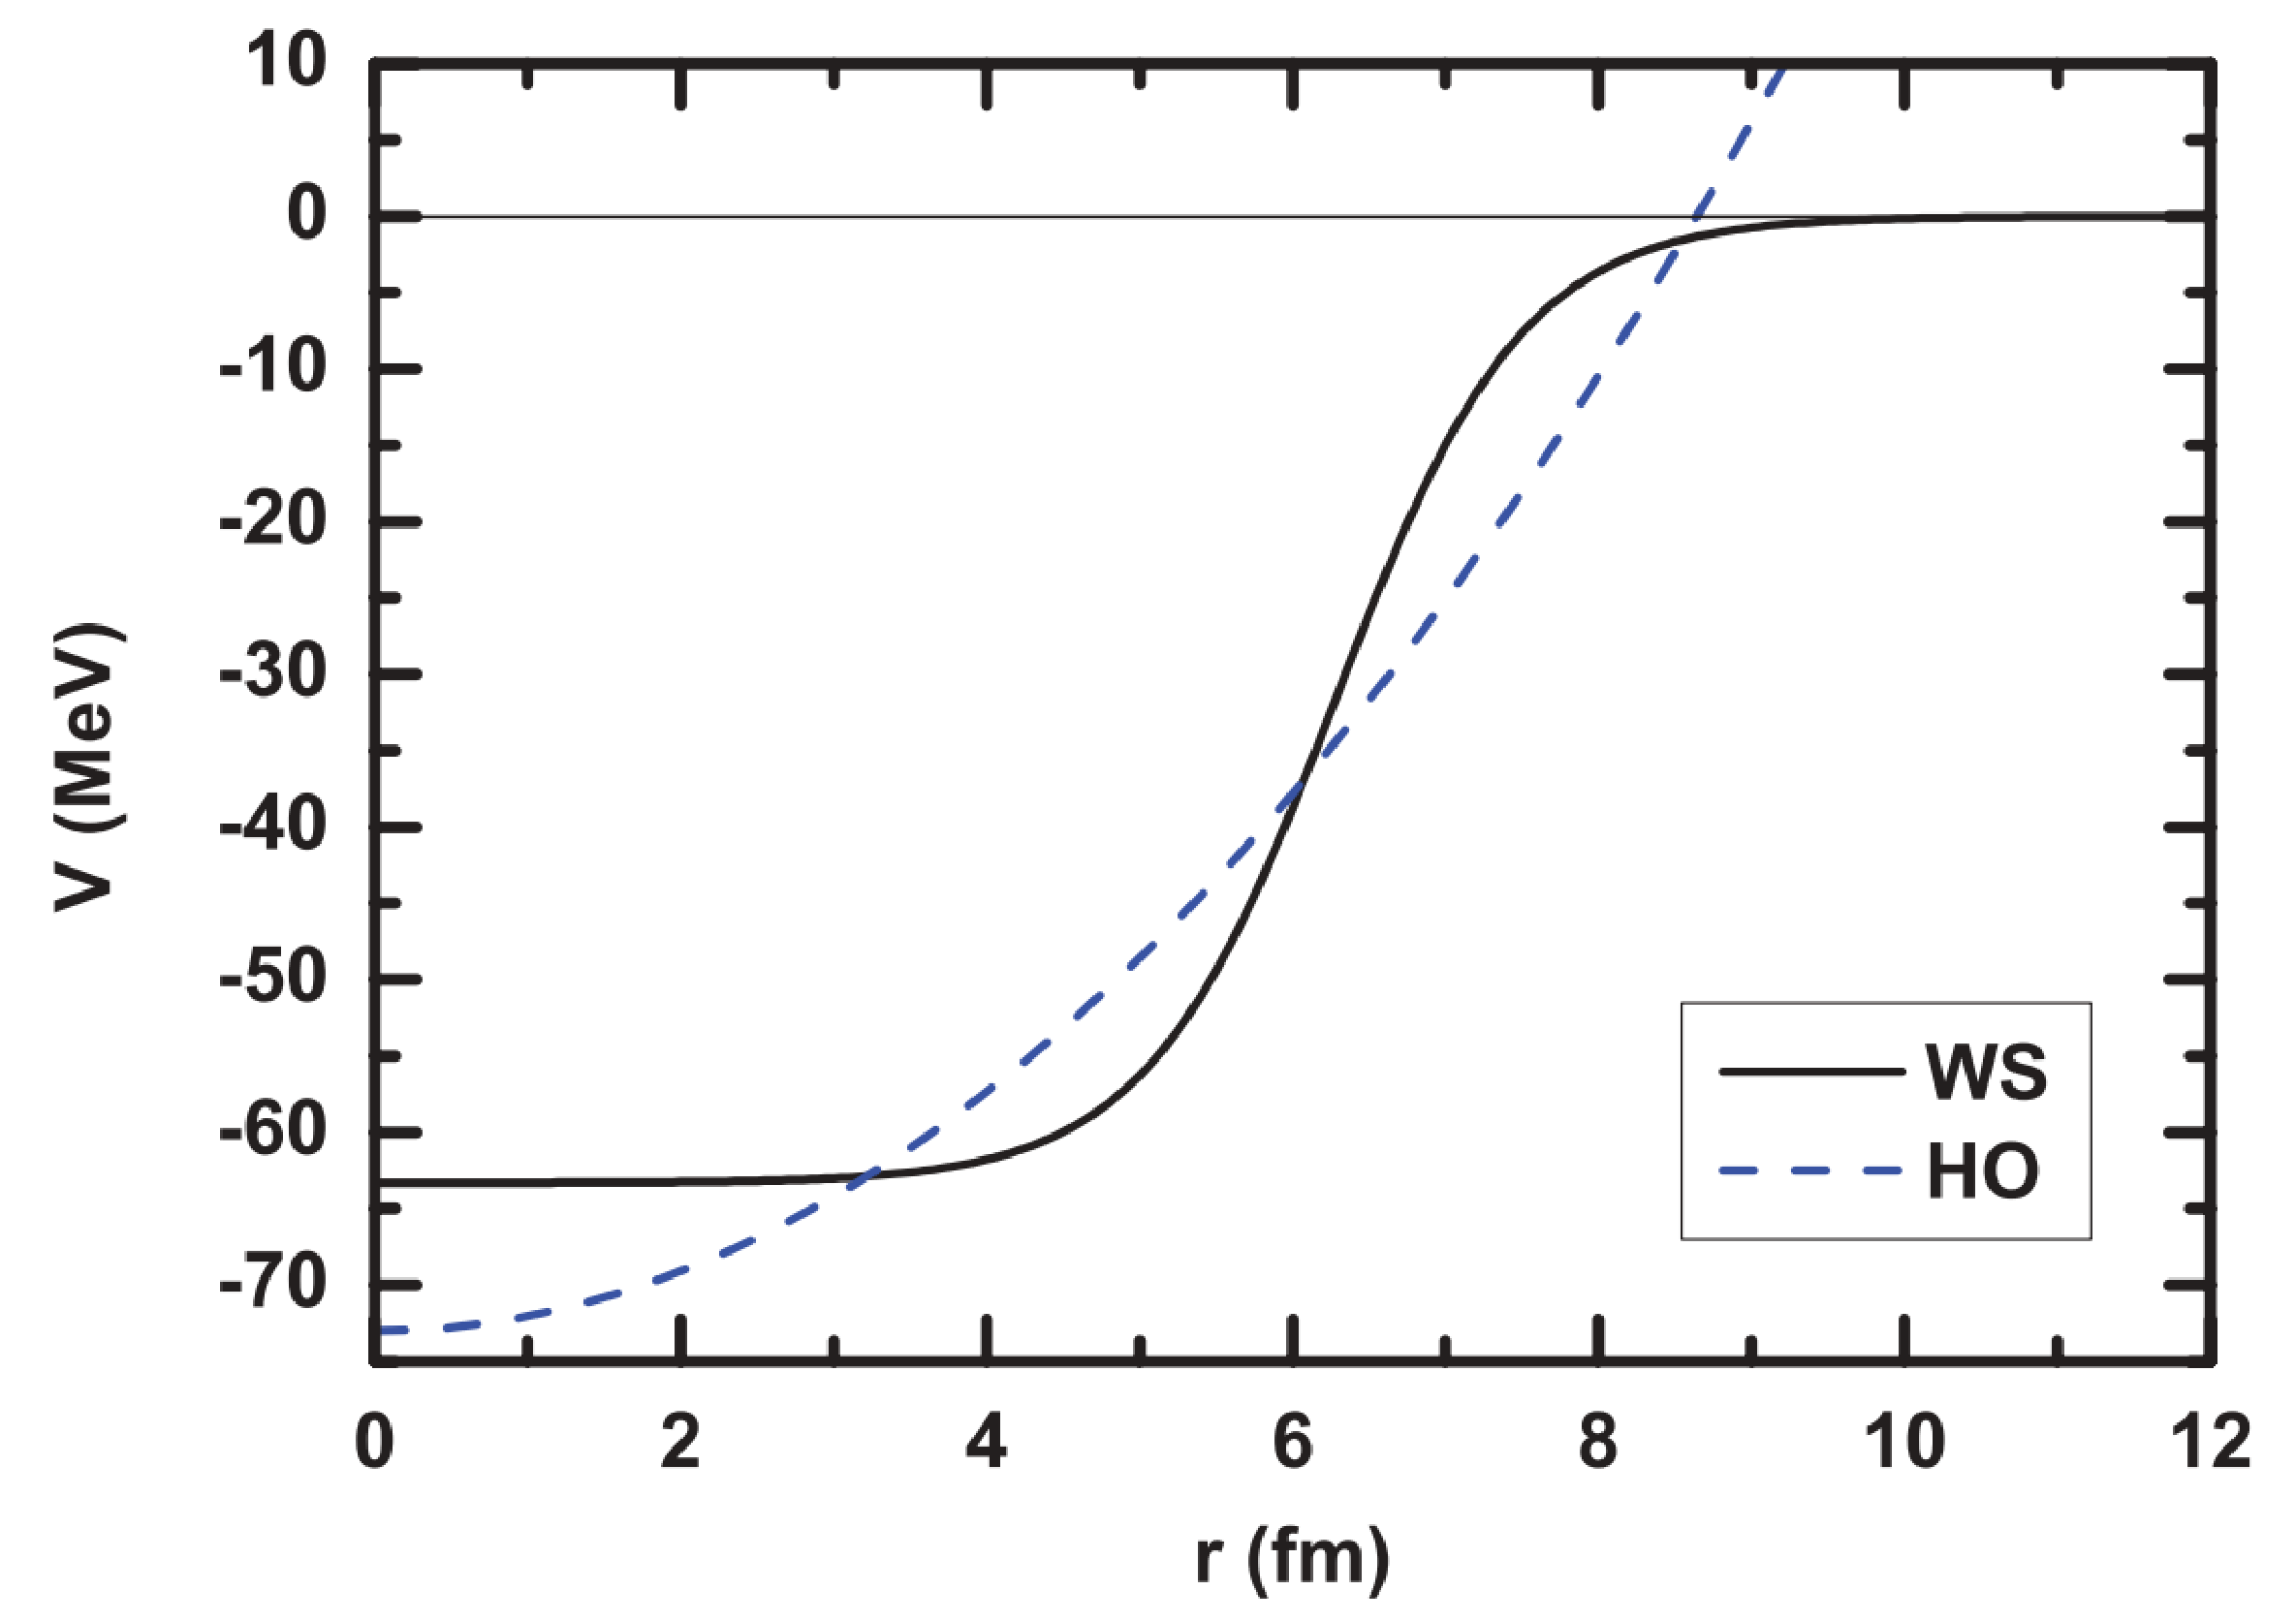
\includegraphics[width=0.8\textwidth]{figures/woodsSaxonVSharmonicOsc.eps}
\caption[The Woods-Saxon nuclear potential.]{A Woods-Saxon potential (solid line) compared to a pure harmonic-oscillator potential (dashed line).  Three parameters describe the Woods-Saxon potential: the well depth $V$, the radius $r_0$, and the surface diffusivity $a$.  Note that the Woods-Saxon potential drops to zero while the harmonic-oscillator potential increases without bound.  From {\refref}~\citep{pseudospinSymmetry}.}
\label{fig:woodsSaxon}
\end{figure}

Understanding the nuclear potential is necessary but not sufficient to begin making predictions about nuclear behavior.  A nucleus consists of many nucleons, all moving within the nuclear potential and interacting with each other; one must describe this many-particle system.  A useful concept in nuclear structure is that of the valence shell of a nucleus.  Nucleons in a filled shell form a $J=0$ core that can be considered largely inert, while the remaining nucleons occupy the valence shell.  The picture is even further simplified due to the strong tendency for nucleons to couple into $J=0$ pairs, so that the ground state of a nucleus can be described simply by describing its unpaired nucleons.  The nucleus of primary interest in this work, \Se{76}, has 34 protons and 42 neutrons.  Like all even-even nuclei, its ground state is \zp, evidencing the strong coupling of nucleons into $J=0$ pairs.  The pairs studied by ($^3$He,n) transfer are proton-pair holes, whose valence orbital is predicted to be $2f_{5/2}$.  While the phenomenological potentials discussed above reproduce trends in nuclear data with some accuracy, the exact wavefunctions of \SeProducts are not known and it can at best be said that the $f$, $p$, and $g$ orbitals are expected to be the primary components of the ground-state wavefunction.  Because the \NME depends on the overlap between the initial and final nuclei, it is desirable to understand these nuclei, and particularly the differences between their ground states, as accurately as possible.  A series of experiments were undertaken to understand these wavefunctions more accurately and will be discussed in {\sect}~\ref{sec:valence}.
\FloatBarrier

\section{Calculation of \NME and Experimental Constraints}

One approach to calculating \NME = $\langle f|O|i \rangle$ is with the shell-model formalism described above.  The difficulty with this approach is that the \zvbb process is spatially confined to $\sim$2-3~fm, which means that intermediate states with excitation energies up to $\sim$100~MeV \citep{anatomy} are relevant to the calculation.  Even though expressing these states with a shell-model basis set can require a space as large as $O(10^{10})$,  several groups have still undertaken this method of calculating \NME \citep{CaurierShellModel}.  Regardless of the method of calculation, the wavefunctions of the initial and final nuclei must impact \NME.  Extensive single-nucleon transfer experiments have been performed to better understand the valence shells and are discussed further in {\sect}~\ref{sec:valence}.

More commonly, calculations of \NME are based on the quasiparticle random-phase approximation (QRPA).  The QRPA provides a framework particularly suited for describing collective excitations.  The random-phase approximation (RPA) uses correlated-particle and correlated-hole annihilation and creation operators to build excited states from a vacuum.  See {\refref}~\citep{Casten} for a readable introduction to the RPA.  QRPA uses quasiparticle annihilation and creation operators instead and assumes that the ground state of the nucleus is in a fully-paired state \citep{BenderSCMF} similar to that of superconductivity as described by Bardeen, Cooper, and Schreiffer (BCS) \citep{BCS}.  See {\refref}~\citep{SuhonenQRPA} for a detailed discussion of the QRPA formalism.  The BCS ground state for even-even nuclei was first suggested by Bohr and Mottelson \citep{nucleiBCS} and is still considered a good approximation for many nuclei \citep{validRegionsBCS_highMass}.  It is known, however, that a BCS vacuum is not always a good approximation to the ground state of a nucleus\citep{NambuBCS}.  In these cases, QRPA calculations can be inaccurate.  Two-nucleon transfer experiments can be helpful in determining the distribution of pairing strength in a nucleus \citep{Yoshida} and therefore support the QRPA assumption of a BCS-like ground state.  See {\sect}~\ref{sec:correlations} for more details on the effect of nuclear correlations on the calculation of \NME. 

\section{Valence Shells of the Initial and Final Nuclei}
\label{sec:valence}
\begin{comment}
\subsection{NME calculations and valence States}
\begin{itemize}
\item (assume that) NME calculations are sensitive to occupied valence states
\item can investigate valence state occupation with transfer reactions
\item \Ge{76} occupancies were experimentally determined and adjusting the energy levels to match changed the NME by a factor of 2 \citep{0vbbReview}
\end{itemize}
\end{comment}
As discussed in {\chap}~\ref{chap:0vbb}, the half-life of the \zvbb process depends on the participating nuclei as well as the neutrino mass scale.  While a direct measurement of \NME = $\langle f|O|i \rangle$ is difficult because it is only accessible by observation of \zvbb, it is possible to study the initial and final nuclear states separately in an attempt to improve the accuracy of the calculations.  

The initial and final nuclear states could inhibit \zvbb if there were significant rearrangement in the neutron or proton shell occupancies.  Single-nucleon transfer is sensitive to the occupancies and vacancies of valence nucleons and therefore an important tool in determining the extent to which the occupancies change between two nuclei.  Very generally, the cross section for transferring a nucleon to a specific shell in a target nucleus will be high if that nucleus has many holes available in that shell but low if that shell is filled.  The Macfarlane and French \citep{sumRules} sum rules state that the sum of occupancies and vacancies for an orbital with angular momentum $j$ must be $(2j+1)$.  This allows determination of valence shell occupancies and vacancies from experimental transfer data.  The validity of the sum rules was recently checked \citep{SumRulesTest} for Ni isotopes, whose valence orbitals are \fpg like \GeTargets.  

It should be noted that while there is extensive transfer-reaction data, it is not all suitable for determining valence shell occupancies because of uncorrelated systematic errors in the absolute cross-sections of complementary reactions.  Comprehensive single-nucleon transfer experiments that are specifically designed to limit these relative systematic errors have been performed on several of the candidate nuclei; see \citep{schiffer_review} for an overview of current progress.  In particular, the nuclei \GeTargets have been studied with the neutron-adding reactions (d,p) and ($\alpha$,\He{3}) as well as neutron-removing reactions (p,d) and (\He{3},$\alpha$) \citep{valenceNeutrons}.  The valence protons of these same nuclei have been studied with the (d,\He{3}) and (\He{3},d) reaction \citep{valenceProtons}.  These studies were done on the nuclei \Ge{74} and \Se{74} as a consistency check.  It was found that the Fermi surfaces of both the protons and neutrons in \GeTargets and \SeProducts are quite diffuse, with the relevant neutron and proton orbits being 2$p_{3/2}$, 1$f_{5/2}$, 2$p_{1/2}$, and 1$g_{9/2}$.  The quantities most important to the \NME calculations are the differences in occupancies between the mother and daughter nuclei; these differences are shown in {\fig}~\ref{fig:occupancyDiffs} along with the theoretical predictions.  The single-particle energy levels were adjusted in the QRPA calculation \citep{SuhonenEnergyAdjust} to provide better agreement with the data.  These changes reduced the QRPA calculation of \NME by approximately a factor of two, bringing it into agreement with the shell-model calculation of \NME.  This reduction in the spread of calculated \NME is particularly valuable to reducing the uncertainty of mass limits or estimates from \zvbb searches. 
\begin{figure}[hp]
\centering
\subfloat[][]{
   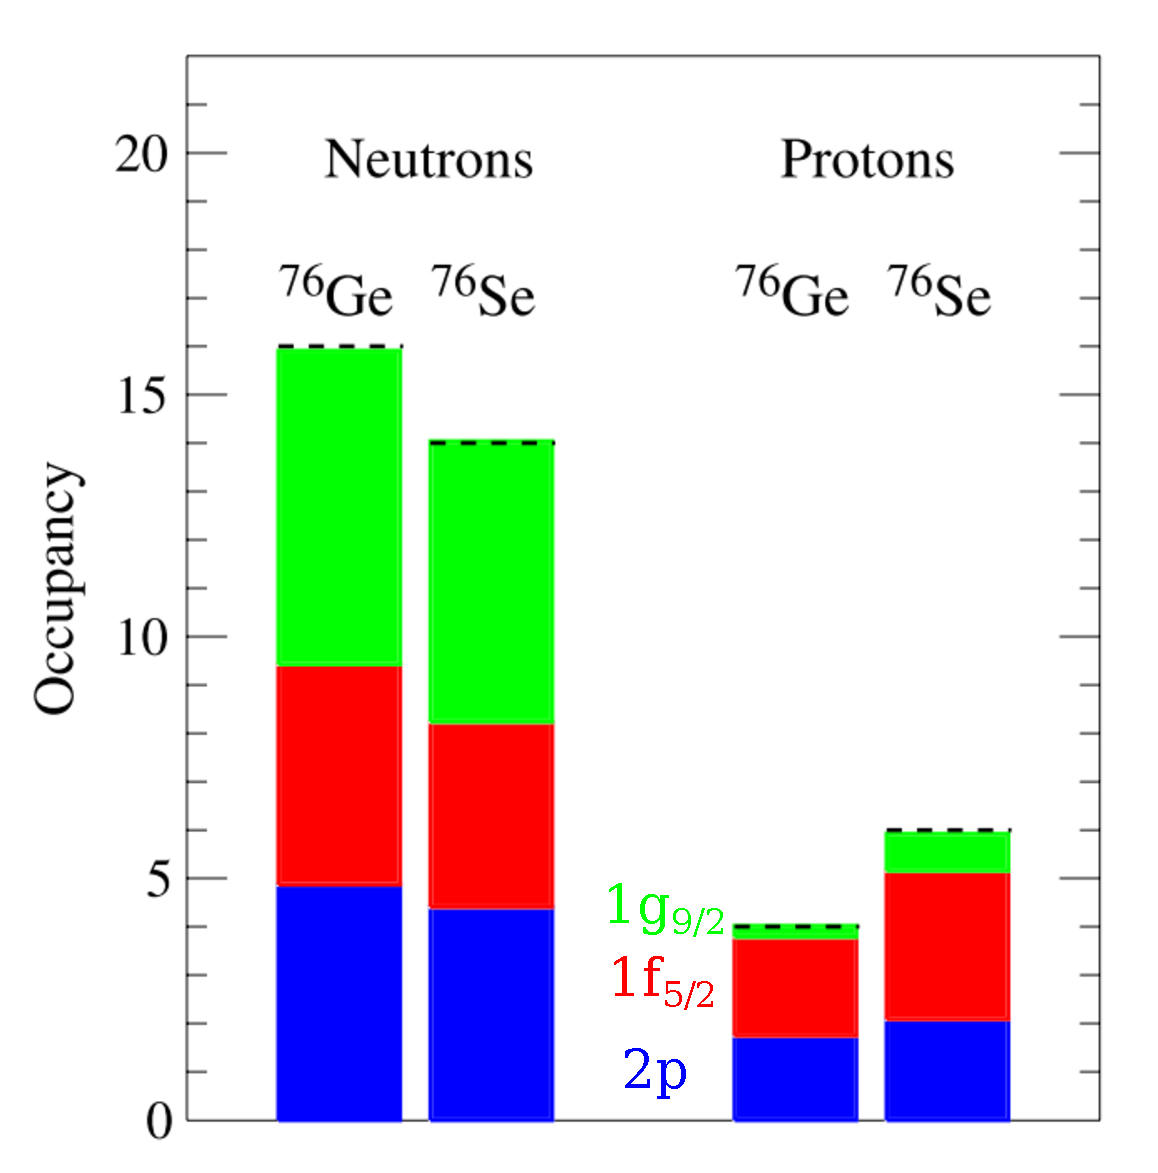
\includegraphics[width=0.4\textheight]{figures/occupancies.eps}
}
\\
\subfloat[][]{
   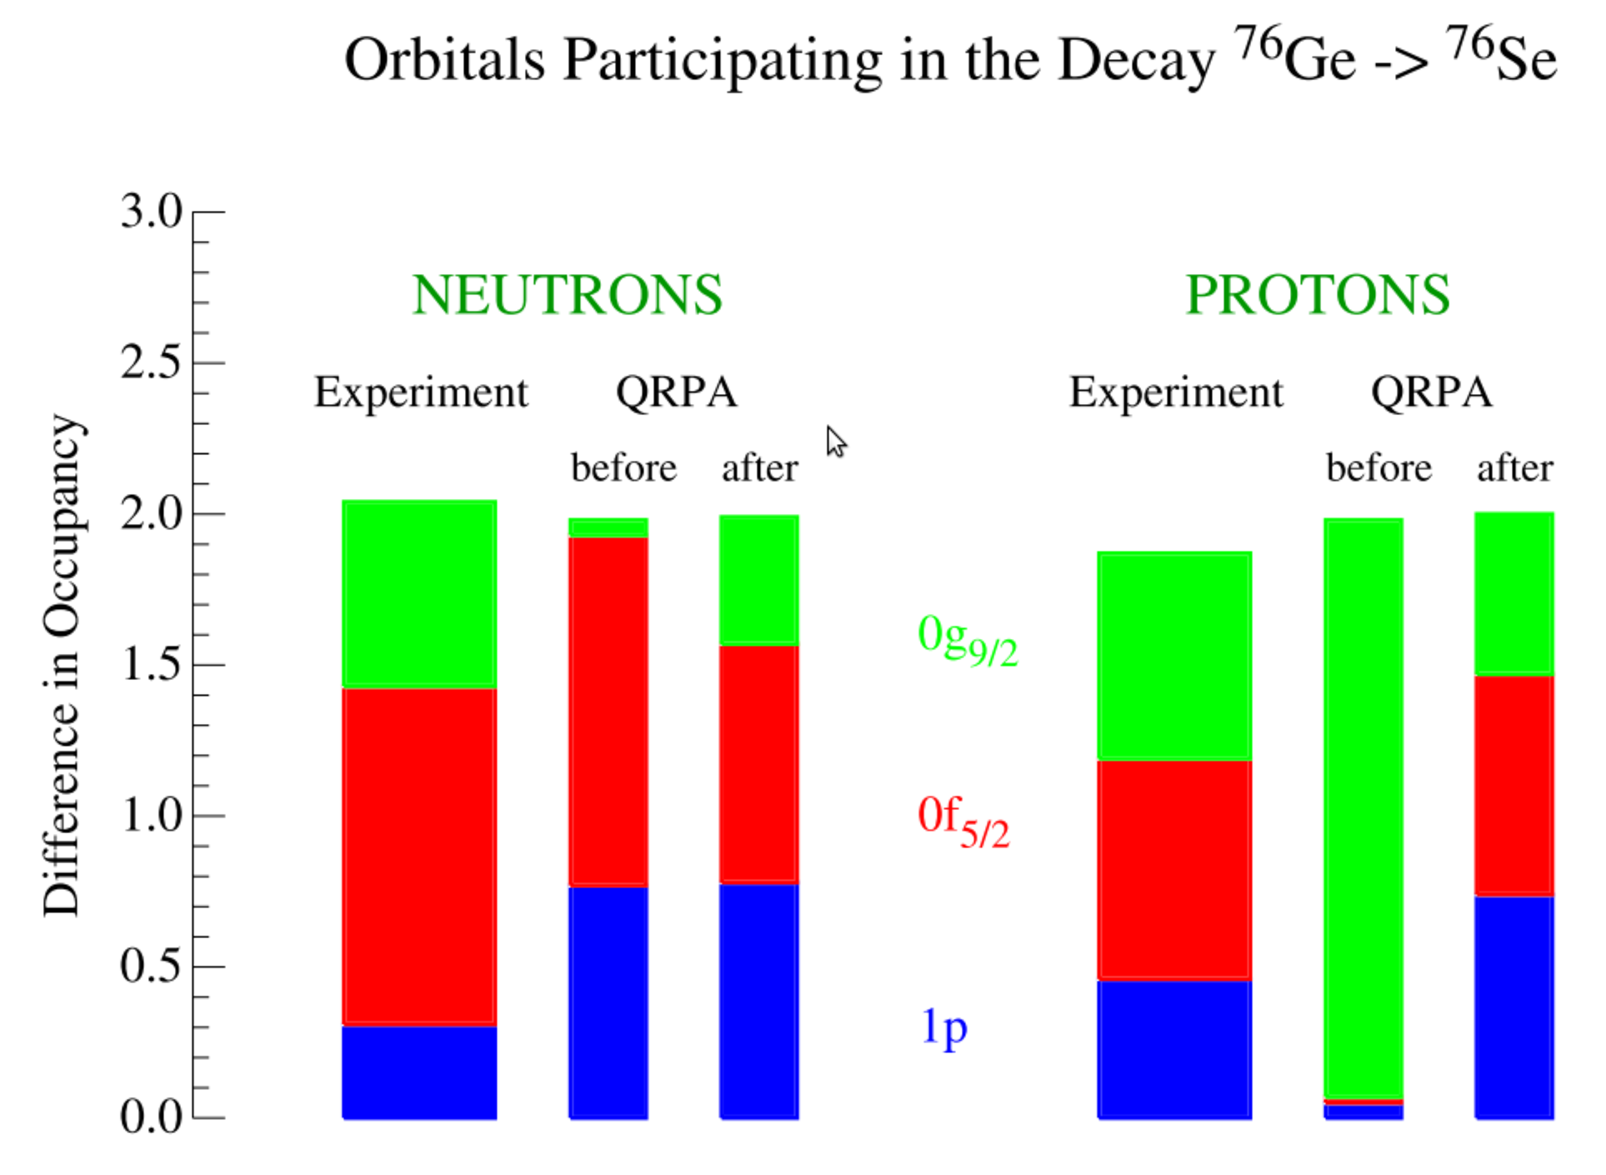
\includegraphics[width=0.4\textheight]{figures/occupancyDiffs.eps}
}
\caption[Occupancies of the neutron and proton valence shells of \Ge{76} and \Se{76}.]{(a) Occupancies of the neutron and proton valence shells of \Ge{76} and \Se{76} determined by single-nucleon transfer reactions.  From \citep{schiffer_review}.  (b)  The differences between occupancies in the final and initial states are determined from (a) and are more immediately relevant to \NME calculations.  The theoretical predictions, before and after adjusting level energies to better match the data, are shown next to the experimental values.  Modified from {\refref}~\citep{schiffer_review}.}
\label{fig:occupancyDiffs}
\end{figure}
\FloatBarrier

\section{Nucleon-Nucleon Correlations and the Impact they have on \NME}
\label{sec:correlations}
\begin{comment}
\begin{itemize}
\item \zvbb occurs on correlated neutron pairs
\item certain pairing in the nucleus can inhibit \zvbb
\item investigate pair correlation with two-nucleon transfer reactions
\item some systems don't have all their \zp in the ground state - Xe
\item discuss neutron transfer experiments done on \GeTargets
\item wish to investigate proton transfer on \GeTargets
\end{itemize}
\end{comment}
In addition to studying the single-nucleon states in \GeTargets and \SeProducts, understanding correlated neutron pairs in \Ge{76} and correlated proton pairs in \Se{76} is relevant to \NME.  Calculations suggest that significant contributions to \NME come from inter-nucleon distances of less than 3~fm \citep{anatomy}.  The distribution of highly-spatially-correlated \zp strength, therefore, may strongly influence \NME.  QRPA calculations can be particularly sensitive to \zp strength that is not exclusively in the ground state as these models assume a BCS approximation where the ground state contains all the \zp strength \citep{BenderSCMF}.  The reaction (\He{3},n) is a particularly useful probe of proton-hole pairing in the target nucleus as the transferred protons strongly populate paired states and thus are sensitive to pairing vibrations \citep{Yoshida}.  The cross section of a two-nucleon-transfer reaction on a nucleus that is well described by BCS should show strong population of the \zp ground-state with little, if any, population of \zp excited states.   

A system that demonstrates the motivation for studying pairing in \Se{76} particularly well is $^{130}$Te, another candidate nucleus for \zvbb.  The neutron-pair (p,t) transfer reaction was used to show that the cross section for excited \zp states is less than 4\% of the ground-state yield \citep{neutronPairsTellurium}, suggesting that a BCS vacuum is a reasonable approximation for the neutrons in ground-state $^{128,130}$Te nuclei.  The same is not true for the proton states; the (\He{3},n) reaction populates an excited \zp state with a cross section that is $\sim$30\% of the ground-state cross section for both $^{128}$Te and $^{130}$Te \citep{protonPairsTellurium}.  Studies of \Ge{76}(p,t) and \Se{76}(p,t) show that the neutron-pairing strength is distributed overwhelmingly to the ground state, with excited-\zp states being populated at less than a few percent \citep{neutronPairsGermanium}.  As can be seen in $^{128,130}$Te, however, the concentration of neutron-pairing strength in the ground state of a nucleus does not imply the same for protons pairs.  The aim of this work is to study the distribution of the proton-pair strength using the two-proton transfer reaction \reaction.  The \Ge{76} target data serve as a check on the results obtained for \Ge{74}, which are the more directly relevant for \zvbb of \Ge{76} because the decay produces correlated proton pairs. 

\section{Modeling Two-Proton Transfers}
\begin{comment}
Discuss DWBA theory of two-proton transfer reactions
\begin{equation}
M\sim\langle\psi_n|V_T|\psi_{^3He}\rangle
\end{equation}
Where $V_T$ is the transfer operator and $\psi$ are elastic scattering wave functions.
Assume that nuclear elastic scattering is the largest contribution to the nuclear reaction and use 1st order perturbation theory to generate $V_T$ from the bound-state wave functions.
To get $\psi$ (?)
\begin{enumerate}
\item treat two particles individually
\item treat two protons as bound cluster
\end{enumerate}
treating particles individually is too complicated
when using cluster model, can adjust $V_0$ of well to match ?? binding energy and adjust $r_0$ to adjust range and $a_0$ to adjust ??.

cluster model's prediction of 0 degree cross section is sensitive to these parameters, but the relative cross sections of \fpg shell nuclei do not depend strongly on the parameters.

Discuss experimental difficulties of two-proton transfer reactions and introduce NSL as a good place to do them
\end{comment}
Measuring differential cross sections can give information about underlying characteristics of nuclei.  For example, population of excited \zp states in two-nucleon transfer reactions gives information about pairing in a nucleus.  However, the calculated cross sections are also influenced by factors not related to nuclear pairing such as kinematics.  These contributions are not as relevant to the calculations of \NME as those that are sensitive to the pairing force.  The distorted-wave Born approximation (DWBA) is used to calculate cross sections of transfer reactions by assuming that nuclear elastic scattering is the largest contribution to the nuclear reaction and that the transfer operator can be constructed from the bound-state wavefunctions of the initial and final states using first-order perturbation theory.  This assumption is particularly accurate for the forward angles which are of interest in this experiment.

A transfer reaction has the form $A (= C+T)+B\rightarrow C+D( = B+T)$ where $T$ is transferred onto the nucleus $B$.  In this work, the reaction of interest is \GeReaction{74}{76}, making the incoming nucleus $A=$ \He{3}, the target nucleus $B=$ \Ge{74}, the product nucleus $D=$ \Se{76}, and the outgoing particle $C$ a neutron.  The transferred nucleons that make up $T$ are a pair of protons.  To perform a DWBA calculation for such a transfer reaction, four potentials are needed: the initial and final-state binding potentials felt by $T$ as well as the potential felt by the incoming nucleus $A$ due to nucleus $B$ and the potential felt by the outgoing nucleus $C$ due to the product nucleus $D$.  DWBA uses optical-model potentials for the latter, which are of the form
\begin{equation}
\label{eq:OpticalModelPotential}
\begin{split}
U(r) = & V_C - Vf(x_0) + \left( \frac{h}{m_{\pi}c} \right) ^2 V_{SO}(\sigma\cdot l)\frac{1}{r}\frac{d}{dr}f(x_{SO}) \\
 & -i[Wf(x_W) - 4W_D\frac{d}{dx_D}f(x_D)],
\end{split}
\end{equation}
where $V_C$ is the Coulomb potential and $f(x_i)=(1+e^x_i)^{-1}$ is the Woods-Saxon potential \citep{PereyPerey}.  The nuclear potential consists of real and imaginary volume and surface terms, written in \ref{eq:OpticalModelPotential} with the coefficients $V$ and $W$ (volume) and $V_{SO}(\sigma\cdot l)$ and $W_D$ (surface).  The variables $x_i$ differ from term to term and are defined as $(r-r_iA^{1/3})/a_i$, where $r$ is the distance from the center of the nucleus, $r_i$ is the reduced radius of a particular interaction, and $a_i$ describes the diffuseness.  The constants $h$, $m_{\pi}$, and $c$ are the Planck constant, the rest mass of the pion, and the speed of light, respectively.  Note that the functional form of the spin-orbit term $V_{SO}(\sigma\cdot l)$ is the derivative of the Woods-Saxon potential, making it predominantly a surface effect.  The imaginary component of the potential allows for absorption and, like the real part, has a volume term $W$ and, in addition, a surface term $W_D$.  The parameters of the optical-model potentials are determined by global fits to elastic scattering data.  Parameter sets that are in common use, such as the Becchetti-Greenlees neutron potential \citep{Becchetti_neutronPotential}, are fits to large sets of data \citep{PereyPerey}.  Potentials to bind the transferred nucleons $T$ (in this work, a proton pair) to their original nucleus $C$ and final nucleus $B$ are also needed and are typically assumed to be a Woods-Saxon potential added to a Coulomb potential.  In the DWBA calculations done in this work, the depth of the Woods-Saxon bound-state potential is varied to match the measured mass of the bound nucleus.
 
When calculating proton-pair transfer cross sections, DWBA calculations can be complicated considerably if one treats each proton in the pair separately.  Bayman and Kallio \citep{BaymanKallio} take this approach, which can accurately predict the absolute differential cross section but also introduces additional parameters such as phases between multi-step transitions.  The many parameters needed for this calculation are poorly constrained unless the wavefunction is well-understood beforehand.  A simpler method, the cluster model \citep{NuclearReactions}, treats the protons as a single, bound cluster.  While this method does not typically reproduce absolute cross sections well, it reproduces the angular distribution of the more-complicated Bayman-Kallio approach, as well as of the experimental data.  It should be noted that, when using either model to predict cross sections, their magnitudes are quite sensitive to the parameters in the Woods-Saxon potential, $r$ and $a$, which describe the radius of the well and the diffuseness of the surface, respectively.  However, the trend of the cross section relative to the energy of the incoming \He{3} or changing neutron number of the target is well-reproduced.

One can use DWBA calculations to understand the kinematic dependence of the expected cross section, as shown in {\fig}~\ref{fig:optimizeCrossSection}; this helps determine an appropriate beam energy.  It can be seen from this plot that the ideal beam energy for maximizing the \reaction cross section is slightly more than 18~MeV.  However, detector resolution decreases with increasing beam energy as discussed in {\sect}~\ref{sec:detector}.  Because the product nuclei \SeProducts have low-lying excited \tp states that could be populated with similar cross section to the ground state, the lower beam energy of 16~MeV was chosen to provide sufficient resolution for resolving these states.  See {\fig}~\ref{fig:levelDiagrams} for level diagrams of the product nuclei.  

\begin{figure}[hp]
\centering
\includegraphics[width=1.0\textwidth]{figures/74Ge_0plus_xsection.eps}
\caption[The $^{74}$Ge($^3$He,n) \zp cross section at zero degrees as a function of beam energy.]{A plot showing a DWBA calculation of the $^{74}$Ge($^3$He,n) \zp cross section at zero degrees as a function of beam energy.  From {\refref}~\citep{schiffer_privateCommunication}.}
\label{fig:optimizeCrossSection}
\end{figure}

As can be seen in {\fig}~\ref{fig:levelDiagrams}, there are known excited \zp states in \SeProducts.  However, these states were discovered through beta decay and excitation due to single-nucleon scattering \citep{NNDC}, neither of which gives information on the distribution of the paired \zp strength between these excited states and the ground state of \GeTargets.  That the leading method of calculating \NME relies on the assumption that the \zp strength is concentrated entirely in the ground state provides strong motivation to experimentally determine this distribution using two-proton transfer.  Particulars of the beam and neutron detector are discussed in {\chap}~\ref{chap:2pExpt} and an analysis of the results in {\chap}~\ref{chap:dataAnalysis}.
\begin{figure}[hp]
\captionsetup[subfloat]{labelformat=empty}
\centering
\subfloat[][]{
   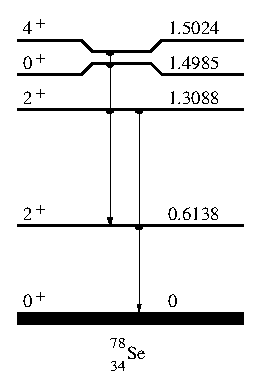
\includegraphics[width=0.3\textwidth]{figures/78Ge_levels.eps}
}
\hspace{2cm}
\subfloat[][]{
   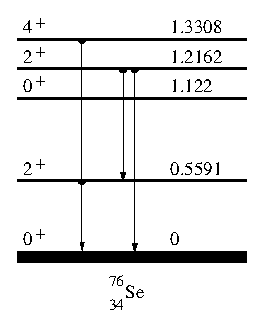
\includegraphics[width=0.3\textwidth]{figures/76Ge_levels.eps}
}
\caption[Level diagram of \Se{78} and \Se{76}.]{The level diagrams of the product nuclei, \Se{78} and \Se{76}.  Note the low-lying 2$^+$ state.  Notice also that both nuclei have known \zp levels.  These levels have been measured through $\gamma$-ray experiments.  Such experiments are not sensitive to the pairing in ground-state nuclei, which is why two-nucleon transfer reactions on \zvbb candidate nuclei are of such interest.}
\label{fig:levelDiagrams}
\end{figure}
% % uncomment the following lines,
% if using chapter-wise bibliography
%
% \bibliographystyle{ndnatbib}
% \bibliography{example}



%
% Chapter 3
%

%
% Modified by Sameer Vijay
% Last Change: Wed Jul 27 2005 13:00 CEST
%
%%%%%%%%%%%%%%%%%%%%%%%%%%%%%%%%%%%%%%%%%%%%%%%%%%%%%%%%%%%%%%%%%%%%%%%%
%
% Sample Notre Dame Thesis/Dissertation
% Using Donald Peterson's ndthesis classfile
%
% Written by Jeff Squyres and Don Peterson
%
% Provided by the Information Technology Committee of
%   the Graduate Student Union
%   http://www.gsu.nd.edu/
%
% Nothing in this document is serious except the format.  :-)
%
% If you have any suggestions, comments, questions, please send e-mail
% to: ndthesis@gsu.nd.edu
%
%%%%%%%%%%%%%%%%%%%%%%%%%%%%%%%%%%%%%%%%%%%%%%%%%%%%%%%%%%%%%%%%%%%%%%%%

%
% Chapter 3
%

\chapter{TWO PROTON TRANSFER AT NOTRE DAME}
\label{chap:2pExpt}

\begin{comment}
Give an overview of the requirements for two-proton transfer and say that ND has a buncher and a Tandem accelerator that goes up to 10 MV so we can get beam energies up to 30 MeV for \He{3} and we have a beamline with a long flight path SO we can do this experiment.
\end{comment}

The previous chapter demonstrated the interest in studying the (\He{3},n) transfer reaction onto \GeTargets ; this chapter will discuss the beam production and experimental setup that are necessary for measuring the angular distribution of this reaction.

\He{3} beam is an excellent candidate for studying two-proton transfer.  The Helium Ion Source (HIS) at Notre Dame can produce 1-2 microamps ($\mu$A) of negatively charged (1-) Helium beam.  To make \He{3} beam, \He{3} gas must be provided to the ion source.  

As discussed in the previous chapter, the purpose of this experiment is to understand the strength of the 0+ ground state.  Maximizing the 0+ cross section requires a beam energy near 18 MeV.  High beam energies come at a cost - the resolution of the neutron detector decreases with increasing neutron energy.  However, the 0+ cross section drops drastically before and after its maximum.  Choosing a lower energy, while increasing resolution, would threaten the ability of the neutron detectors to see any signal at all above noise.

The resulting products of a two-proton transfer onto \Ge{76} are a neutron and a \Se{78} nucleus.  While the heavy, charged \Se{78} nucleus is unlikely to escape the target, the escaping neutron provides a way to study this reaction.

Searching for states based on angular momentum can be effectively done with detectors that are segmented in angle, providing a differential cross-section.  Because the states of interest are 0+ states, the angular range most important to cover is 0 to 22 degrees, the maximum and the minimum of the differential cross section.  The neutron detector consists of 16 independent plastic bars, each spanning approximately 1 degree, from 7 degrees to 22 degrees as shown in figure ??.

% figure: detector setup

The Tandem Van deGraaff accelerator at Notre Dame has a maximum terminal voltage of 10 mega volts (MV).  Beam extracted from the HIS is singly, negatively ionized by Lithium vapor.  The beam stays in this ionization state until it encounters a carbon foil in the center of the accelerator terminal and is stripped of all its electrons, leaving it \He{3}$^{2+}$.  In the case of \He{3} beam, then, the energy of the accelerated beam with a terminal voltage of $V_T$ is 

\begin{equation}
E = 3V_T
\end{equation}

For 16 MeV \He{3} beam, the terminal voltage required is 5.33 MV, easily provided by the accelerator, but neutron detection imposes an additional constraint on the beam.  The resulting products of a two-proton transfer onto \Ge{76} are a neutron and a \Se{78} nucleus.  Our detector has a relatively small neutron detection efficiency, but the heavy, charged \Se{78} nucleus is unlikely to escape the target, forcing us to rely on neutron detection to study this reaction.  

Imagine for a moment the options that are available to the neutron that wishes to interact with any detector.  It has no charge, so disturbing electrons via the electromagnetic force is not possible.  The neutron can interact with the electrons weakly, but this probability is impractically small.  A neutron may also interact with a proton, strongly.  This strong interaction is predominantly responsible for neutron detection.  A neutron that transfers some of its energy to a proton can rely on the charged proton to interact with the solid's electrons and register a signal in the detector.  What experimenters must do is provide plenty of protons for neutrons to collide with - large quantities of water or plastics, with their long hydrocarbon chains, are popular choices.

What does a neutron signal look like in such a detector?  If the neutron always deposited its full energy in the detector, the energy spectrum would show sharp peaks corresponding to each neutron energy.  However, a neutron interacting with a proton only transfers all its energy to that proton in a head-on collision.  Monoenergetic neutrons will deposit a range of energy in the detector, from no energy at all to their full energy.  This makes it impossible to determine the energy of the neutron from its deposited energy.  In this transfer experiment, it is necessary to distinguish neutrons with different energies.  Because the neutron's deposited energy does not determine that neutron's full energy, the experiment must be sensitive to some quantity that gives unambiguous information about the neutron's energy.

% figure of charged-particle energy spectrum
% figure of neutron energy spectrum

The neutron energy uniquely determines the time it takes for the neutron to travel from the target to the detector in \eq \ref{eq:TOF}.  

\begin{equation}
\frac{v}{c} = \sqrt{\frac{E^2 - m^2c^4}{E^2}}
\label{eq:TOF}
\end{equation}

Measuring the time of flight (TOF) of the neutron to sufficient accuracy requires both beam bunching and a long neutron flight path.  In a continuous beam, there is no way to know which \He{3} was associated with a neutron event in the detector, and therefore no way to determine TOF.  Bunching the beam so that clumps of \He{3} arrive at the same time and providing a signal correlated to their arrival at the target allows a TOF measurement with a precision determined by the time-width of the bunch.  This limit on time resolution constrains the distance between the target and detector.  The flight path must be long enough to distinguish ground state neutrons from neutrons associated excited states of the residual nucleus.  In the case of \Ge{76},  the energies of the ground and first excited state neutrons differ by only 0.5 MeV out of $\sim$25 MeV.  With a flight path of 1 m between the target and detector, the difference in time between these two neutrons is ?? ns - far less than the resolution determined by the beam bunch.  In all experiments discussed, the flight path is approximately 15 m, the largest allowed by the room, to maximize energy resolution.  

\section{Beam Production at Notre Dame}
The beam delivered to the target is 16 MeV bunched \He{3}.  In this section, we will follow the beam through its production and accelaration.

The accelerator at Notre Dame is a Van deGraaff accelerator made by High Voltage Engineering Corporation.  Its maximum terminal potential is 10 MV.  Beam enters the accelerator negatively charged and accelerates toward the positive terminal, located in the center of the machine. A thin carbon foil ($\sim$ 3 $\mu$g/cm$^2$) in the center of the machine strips the electrons from the beam.  The now-positive beam accelerates again, away from the positive terminal.  

The Helium Ion Source (HIS) provides negative \He{3} ions to the accelerator.  A duoplasmatron ion source filled with \He{3} gas uses a discharge across high voltage to convert some of the gas into plasma.  Electrostatic elements extract the plasma into a canal filled with lithium vapor.  Lithium is crucial to creating negatively charged beam because it donates electrons generously, and some \He{3} becomes ionized after passing through the canal.  A dipole magnet after the ion source removes the carbon, oxygen, and other impurities that contaminate the \He{3} beam.  Movable, thick tungsten slits block much of the beam, allowing only beam within a small range of magnetic rigidity to pass through to the accelerator.

The accelerated beam again encounters a large dipole magnet that selects beam of the desired energy.  The magnetic field strength is adjusted using the nuclear magenetic resonance (NMR) of hydrogen and leaves the beam with an energy spread of approximately 10 keV.  Comparing this energy spread to the energy spread introduced by the target gives a sense of how small the error associated with the beam energy is; the target spreads the energy by 0.5 MeV.

\subsection{Beam Focusing and Selection}

The accelerated beam must travel in vacuum from the accelerator to a target.  Many focusing and steering elements along the way are necessary to obtain a reasonable transmission rate.  Two Einzel lenses [need cite] focus the beam before it enters the accelerator, and a set of electrostatic steerers before and after the accelerator are enough to position the beam before it enters the energy-selecting dipole magnet.

Quadrupole doublet magnets focus the beam as it travels through the target rooms, and another set of steerers allows correction of the beam position and angle.  The final focusing element before the target are two large-bore, variable-strength solenoid magnets [cite needed] that focus the beam to a spot approximately 2 mm in diameter.

% figure: beamline
\begin{figure}[htp]
\centering
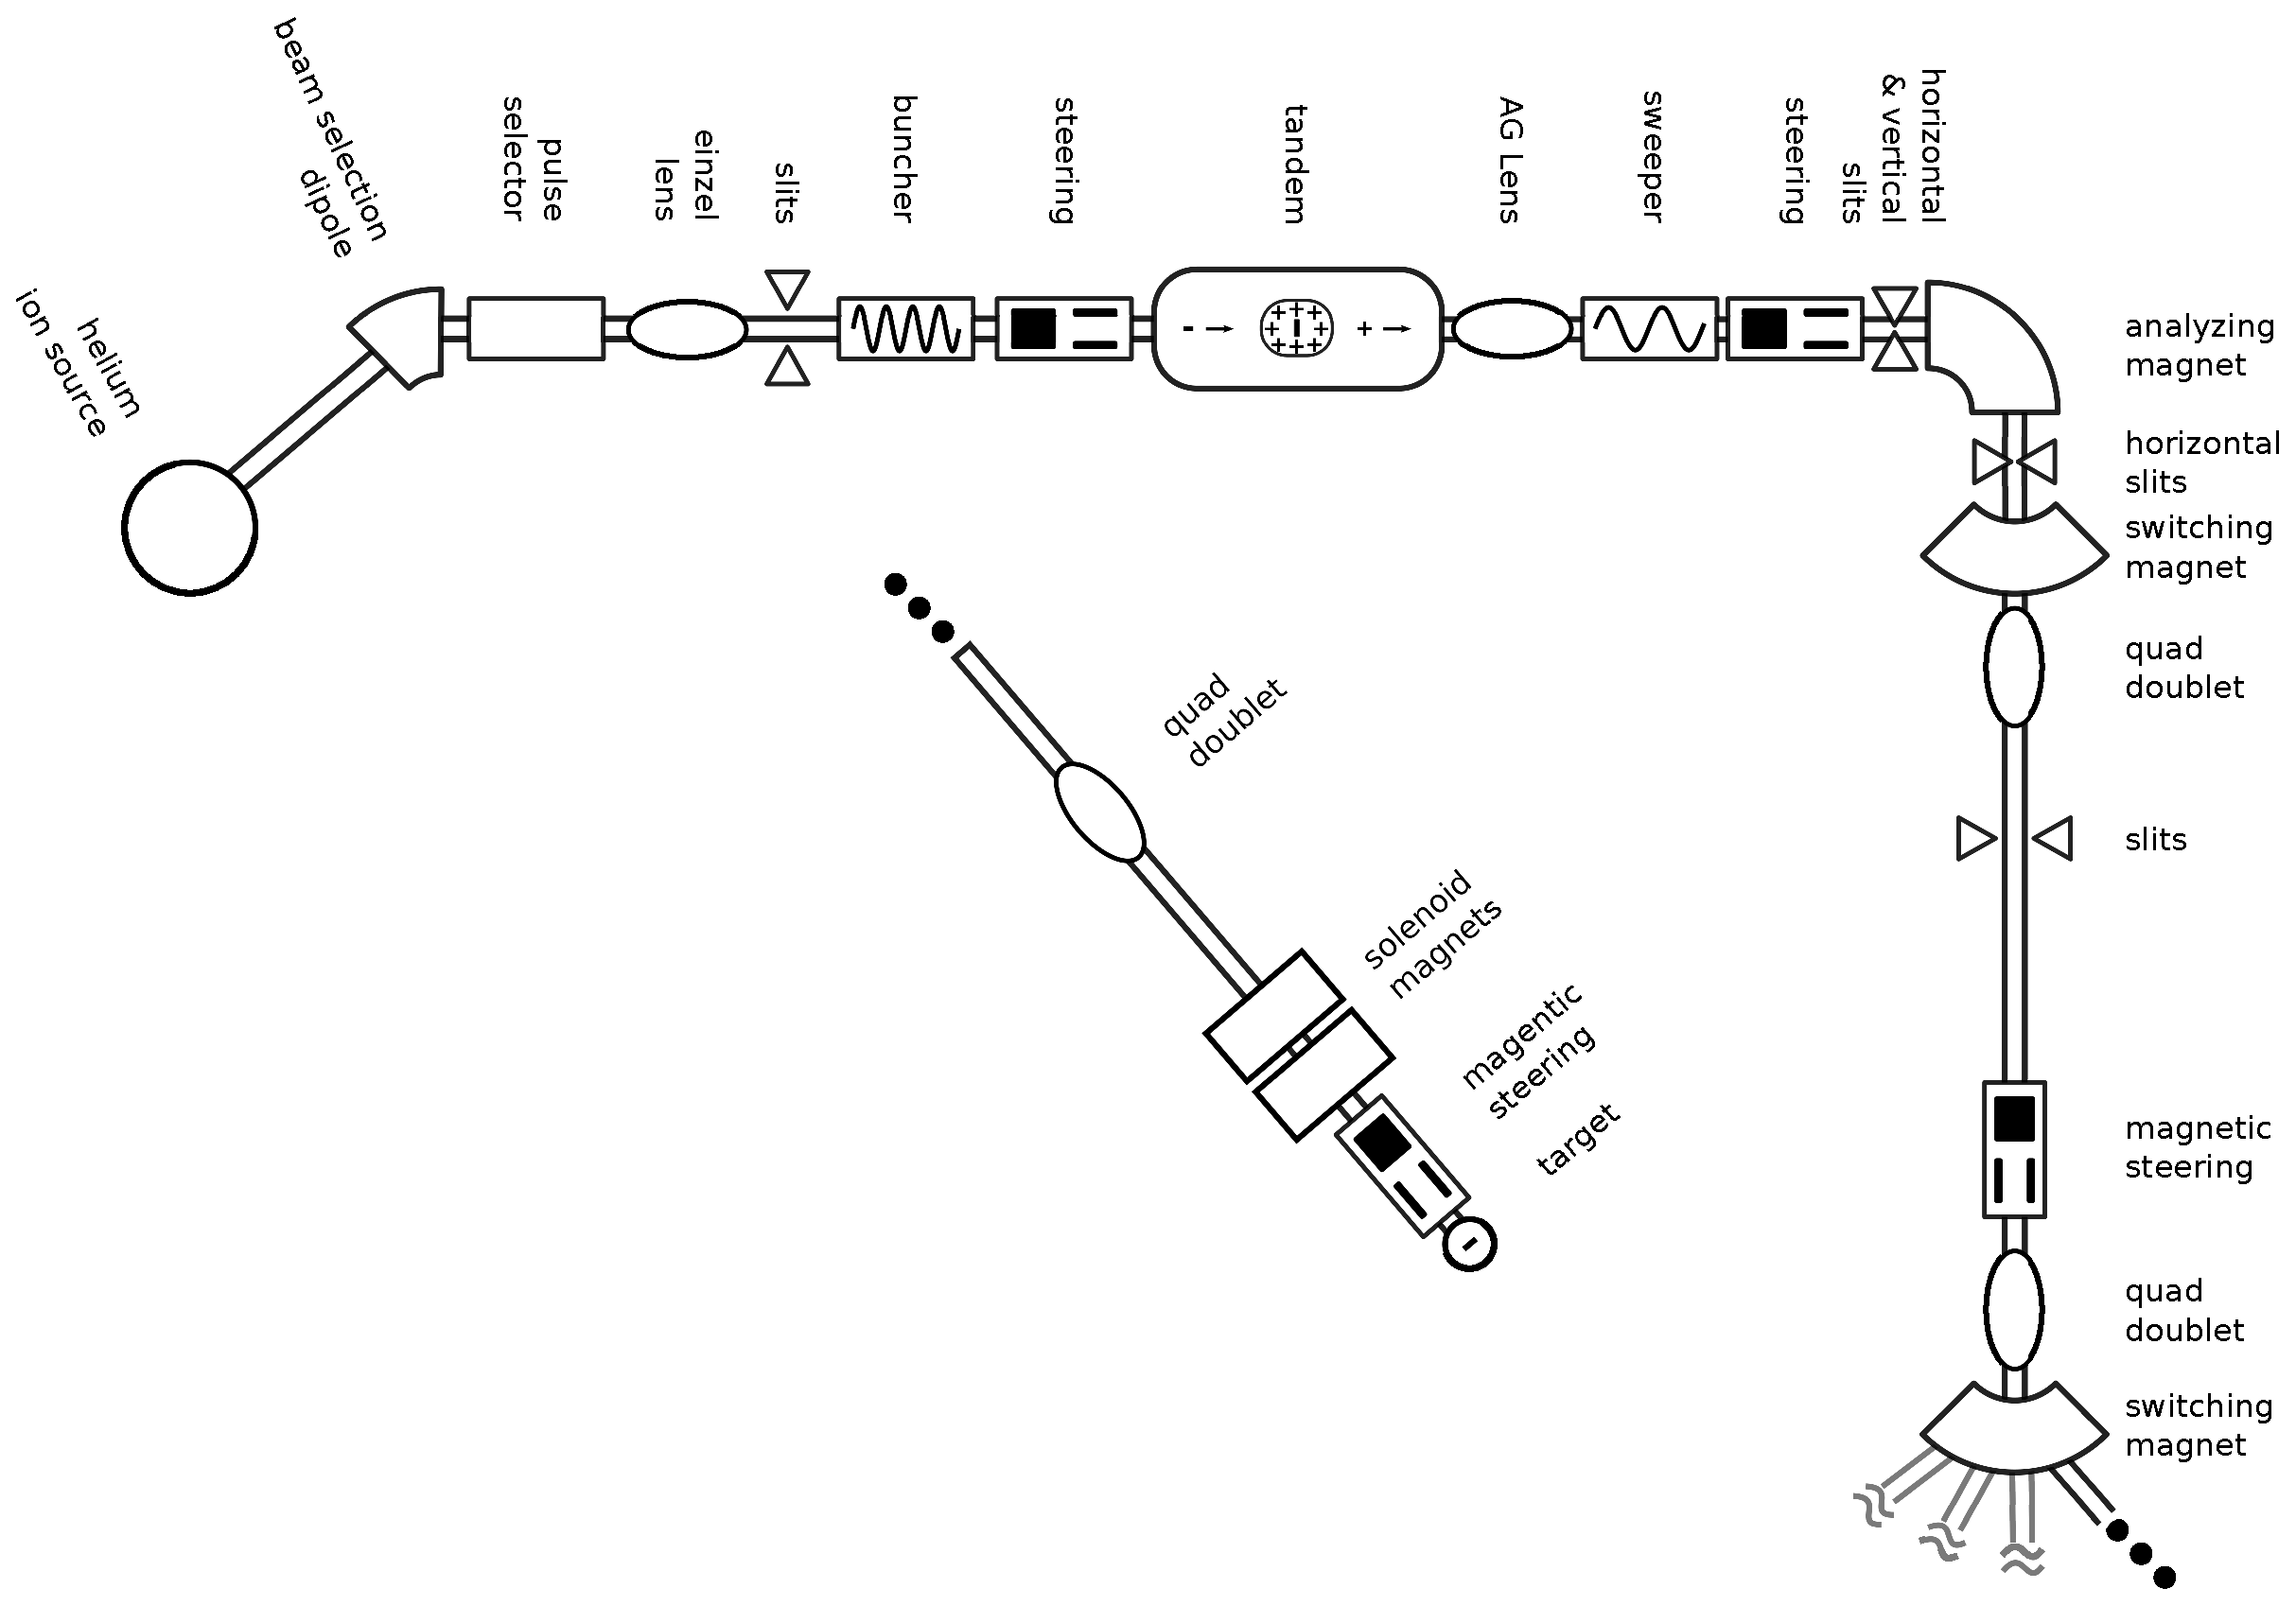
\includegraphics[width=1.0\textwidth]{figures/NSL_beamline.eps}
\label{fig:beamline}
\caption{Beam production at Notre Dame.}
\end{figure}

\subsection{Beam Bunching}

Continuous beam would make it impossibile for our detectors to determine the neutron TOF.  It is possible to bunch the beam so that ``bunches'' of \He{3} arrive at the target, each bunch having a time spread of approximately one ns.  

The beam buncher at Notre Dame works by slowing down particles that would arrive too early at the target and speeding up particles that would be arriving too late.  To acheive this, two grids perpendicular to the beam connect to a radiofrequency (RF) power supply to create an intense electric field that varies in time.  If the electric field were a sawtooth wave in time, the beam bunches would contain all the beam.  Commercially available RF power supplies providing adequate current and rapid enough signal, however, generally vary sinusoidally in time.  At some beam facilities \cite{LynchBunching}, multiple RF amplifiers provide additional frequncies, better approximating a sawtooth wave.  A ``triple-harmonic buncher'' \cite{LynchBunching} generates the correct amplitude, frequency, and phases of the first three Fourier components of a sawtooth wave, which results in adequate bunching of $\sim$80\% of the incident unbunched beam.  However, this requires several expensive RF amplifiers and complicated control electronics.  At Notre Dame, a single frequency buncher that operates at 9.85 MHz is used.  The best bunching occurs while the RF signal is increasing approximately linearly with time; when the electric field is decreasing, de-bunching occurs.  At the target, nanosecond (ns) wide bunches contain $\sim$40\% of the beam and arrive at the target every 101 ns on top of the remaining continuous beam.  This continuous beam would render our time signal useless and must somehow be removed.

% figure: how a beam buncher works
\begin{figure}[htp]
\centering
\includegraphics[width=1.0\textwidth]{figures/beamBunching.eps}
\label{fig:bunching}
\caption{Beam bunching using a varying electric field.}
\end{figure}

The ``sweeper'' provides a large electric field that ramps up and down very quickly to remove the unwanted beam between the bunches.  While conceptually simple, the time scale required for the charging of the plates makes it difficult to find a commercially available power supply.  The field must turn ``on'' on a timescale much smaller than the beam bunch, or else become the limiting factor in the time-width of the bunch.  The power supply used provides ?? charge in ?? ns.

%figure of beam profile and sweeper

At Notre Dame, the beam bunches are 101.5 ns apart and are typically 1 ns to 2 ns wide.  This bunch spacing presents a problem for the experiment because the spread in TOF of the neutron spectrum is in excess of 200 ns.  With bunches arriving at the target every 100 ns, it will be impossible to tell if a neutron is very fast and associated with the current bunch or very slow and associated with the previous bunch.  The spectrum will be considerably complicated by this ambiguity, as shown in Figure \ref{fig:PSvsNPS_TOF}.

% figure: the considerably complicated spectrum
\begin{figure}[htp]
\centering
\subfloat[][]{
   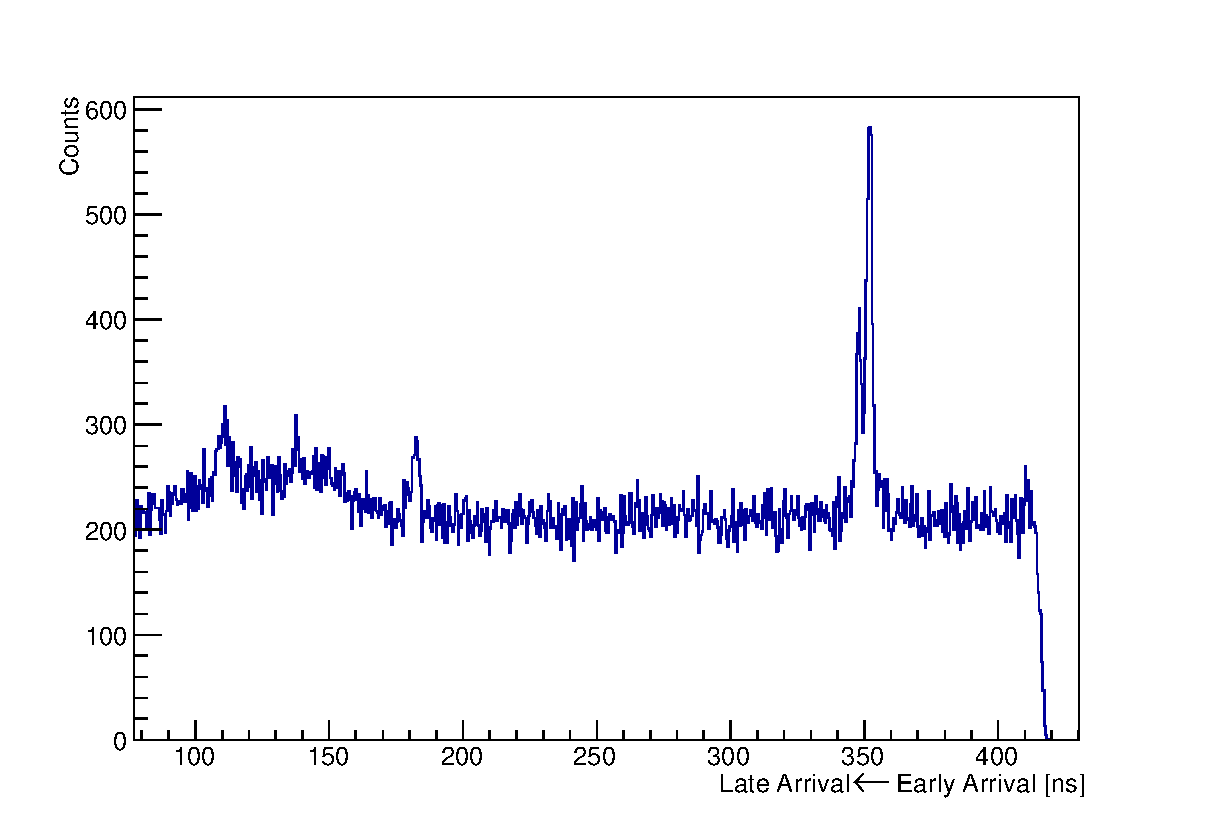
\includegraphics[width=0.4\textwidth]{figures/PS_BarA_Sep.eps}	
}
\subfloat[][]{
	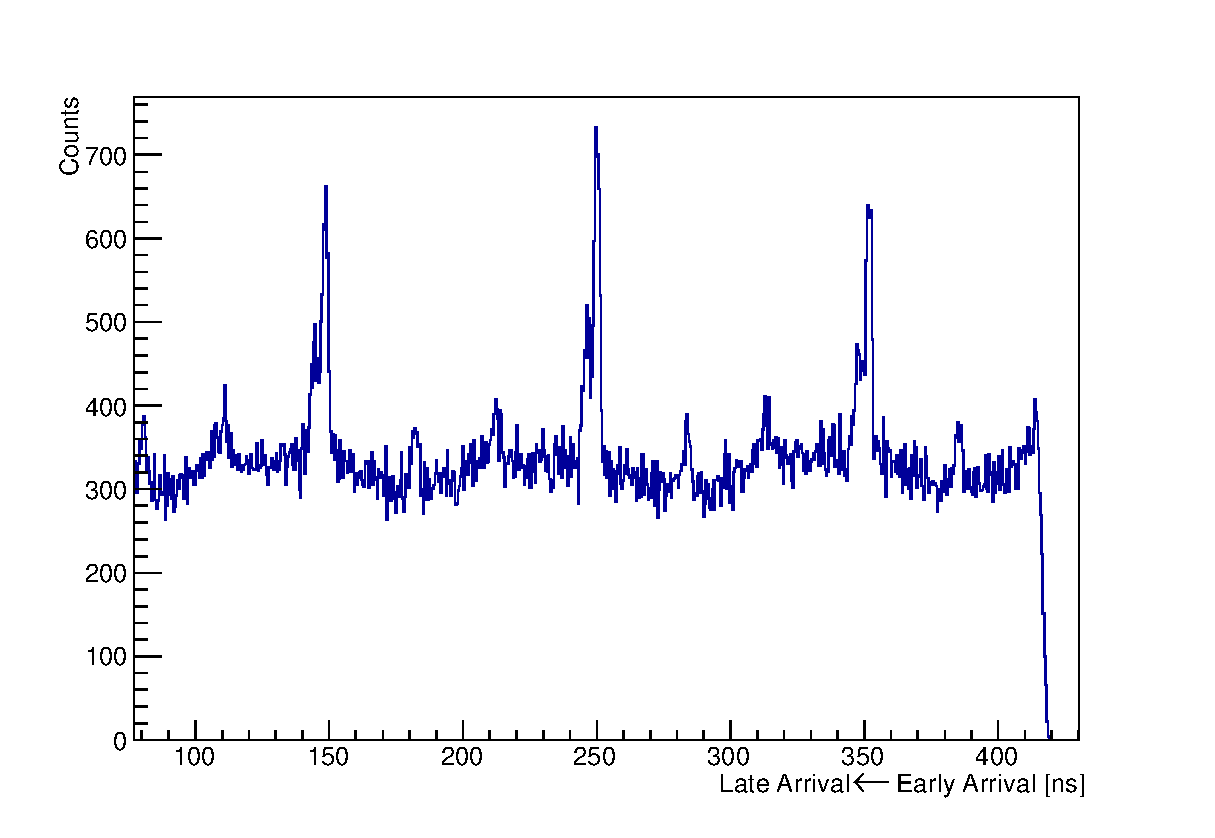
\includegraphics[width=0.4\textwidth]{figures/NPS_BarA.eps}
}
\label{fig:PSvsNPS_TOF}
\caption{Figure A shows timing spectrum from a pulse-selected beam.  The timing spectrum in figure B is from beam with no pulse selection.  Both timing spectra are from a \He{3} beam on a \Ge{76} target.}
\end{figure}

To give all the neutrons resulting from one beam bunch time to reach the detector before the next bunch strikes, a ``pulse selector'' eliminates three of every four bunches, resulting in 400 ns between each bunch at the cost of beam intensity.  Even with 400 ns between bunches, very slow neutrons from previous bunches overlap with $\gamma$ rays from the current bunch, but these are eliminated by placing an energy cut that selects against very low energy neutrons.

% figure: slow neutrons and their dissappearance

Beam bunching and pulse selection dramatically reduces available beam - the swept beam current is only 40\% $\times$ $\frac{1}{4} = 10$\% of the non-bunched current.  But without bunched beam it would not be possible to distinguish the neutrons of interest in the (\He{3},n) transfer reaction.  As it happens, however, the Notre Dame facility cannot improve the statistics of this experiment by very much because the radiation limits on the room with the detector are so low that even with pulse selection, the beam is near its maximum allowed current.

\section{The Target Chamber}
\begin{comment}
target
thin stainless stell wall
Si detector
BaF2 detector
\end{comment}


\section{The Neutron Detector}
\begin{comment}
Discuss neutron wall briefly.  Can reference NIMA paper. Explain why it's important that it's wide-angle. 
Electronics diagram!  Discuss two most important aspects: TDC and ADC from phototubes
\end{comment}

The neutron detector consists of 16 large (1.5 m $\times$ 0.15 m $\times$ 0.05 m) bars of commercially available scintillator [reference BC408?].  The detectors sit in a rough circle with a radius of $\sim$15 m centered around the target.  The forwardmost angle relative to the beam is 5$^{\circ}$ and the largest angle is $21^{\circ}$.  The angle step size between each detector is approximately 0.7$^{\circ}$.  The detectors sit 14.6 m away from the target to ensure a resolution of at least 0.5 MeV at 22 MeV.  At this distance comes the solid angle of each detector is only 10 cm/15 m $\times$ 2.5 m/15 m = 0.11 sr.

% figure - picture of detector

The plastic scintillator bars are each equipped with two photomultiplier tubes (PMT's) with signal risetimes of approximately 5 ns.  Because the PMT's have such a fast risetime, they provide excellent timing information as well as energy information.  Energy deposited is not useful for neutron identification; it is timing information that indentifies neutrons.  In principle, the timing information is all the data acquisition (DAQ) needs to record.  This would be true if there were no background radiation, but concrete in the room emits low-energy $\gamma$ radiation that leaves signal in the detector at a high rate.  Measuring the energy deposition is necessary because it allows us to eliminate this low-energy background radiation.  

While energy information is necessary, it does not need to be terribly precise.  The timing information, however, is the only information useful for neutron identification and must be as precise as possible.  The goal for the electronics is to not add spread to the timing that is noticable above the timing spread already inherent in the beam bunching.  This is why the detectors are equipped with PMT's that have excellent timing response.  The 5 ns PMT signal risetime, together with Constant Fraction Discriminators (CFD's), give timing information with jitter that is about 1 ns.

% figure: CFD operation

\subsection{Electronics}
When a real event occurs in some bar of the neutron detector, the DAQ must record the energy and time of both the top and bottom PMT of that bar.  A charge to digital converter (QDC) can integrate the PMT signal and a time to digital converter (TDC) can measure the time between a logic pulse created by the PMT signal and the logic pulse from the beam buncher.  Because time resolution is crucial, constant fraction discriminators (CFD's) and not leading edge discriminators create the logic pulse sent to the TDC.  

The lone signal provided by the PMT base is not adequate for this processing because two signals, one for the QDC and one for the TDC, are necessary.  The signal from the PMT base is also too small to trigger the CFD's.  The $\times$10 amplifier makes the signal large enough to trigger the CFD's and provides two copies of the input signal, one which can be analyzed for timing information while the other is analyzed for energy information.  A simplified diagram of the data acquisition is shown in fig \ref{fig:simpleElectronics}.

% figure: simple electronics
\begin{figure}[htp]
\centering
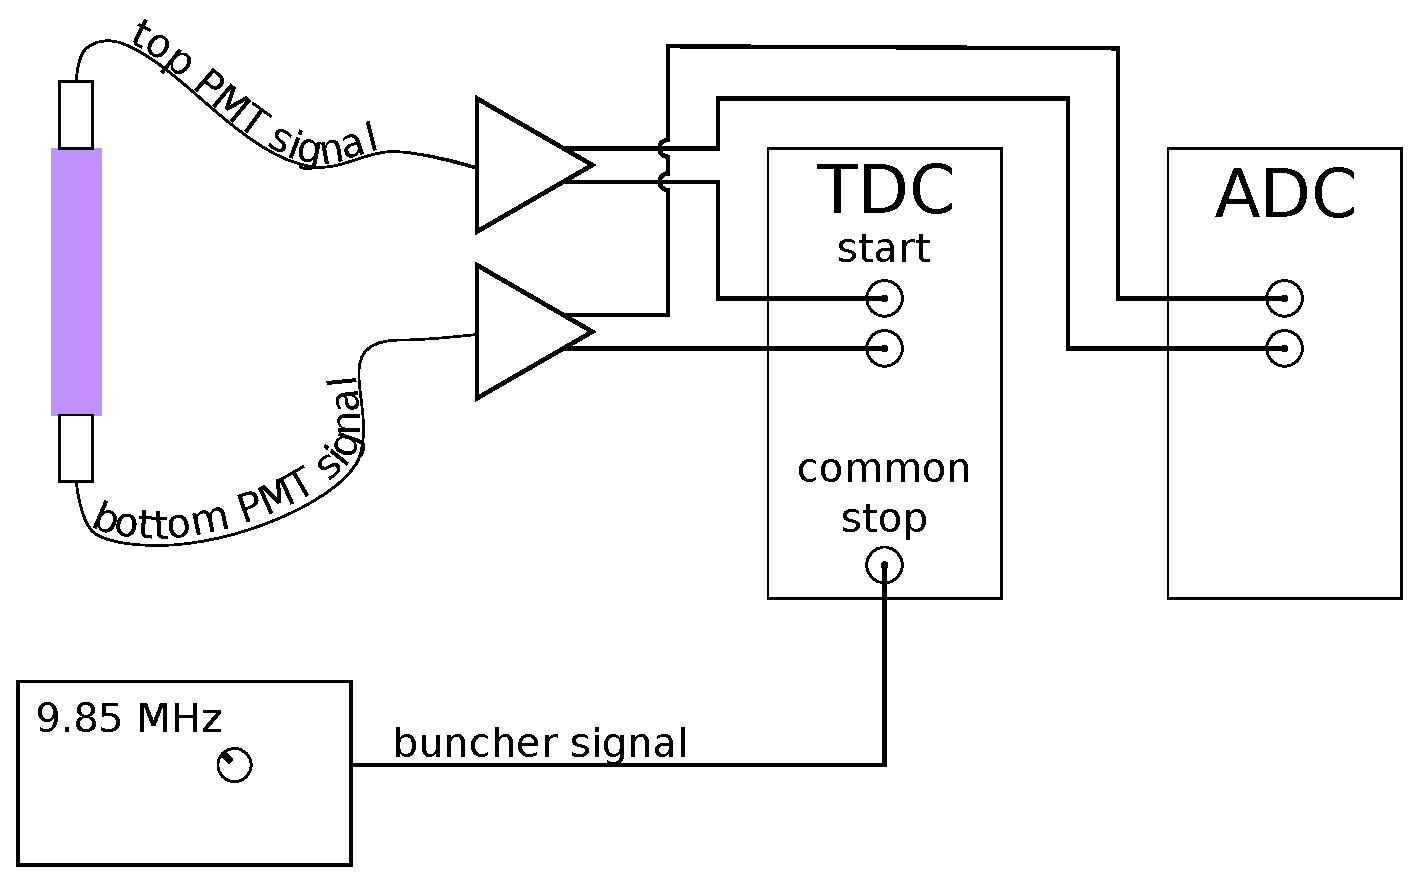
\includegraphics[width=1.0\textwidth]{figures/basic_electronics.eps}
\label{fig:simpleElectronics}
\caption{A simplified diagram of the neutron detector electronics showing the acquisition of timing and energy information from the detectors.}
\end{figure}

What is a good trigger to construct for the neutron wall?  For just one neutron detector, triggering any time the top or bottom PMT fired would waste the DAQ with recording many noise events.  A real event should create signals in both the top and bottom PMT's, and requiring a coincidence between the two results in a reasonable trigger.  One way to define an event trigger for the entire neutron wall, then, would be to trigger any time a coincidence between associated top and bottom PMT's occurs.  But constructing this trigger with NIM logic units requires 16 separate logic gates and would require purchasing additional, expensive logic modules.  

The solution is to use the built-in OR of the CFD.  Instead of requiring a top and bottom signal in the same bar, the condition is loosened to requiring a signal in a top PMT and a bottom PMT in the same eight-bar group.  Each CFD is an eight-fold unit that receives only top or bottom signals and provides an OR output.  The presence of some top signal AND some bottom signal triggers the event signal.  Such an event only requires that both a top and a bottom signal coincided but does not require that these signals belonged to the same bar.  Such an event trigger includes all events of interest, where the top and bottom signal belong to one bar, but also includes spurious events where no bar has signal in both its top and bottom PMT.  With a dead time of less than 30\%, this event condition does not hinder data collection, and simple software cuts eliminate spurious events.

% figure: event trigger
\begin{figure}[htp]
\centering
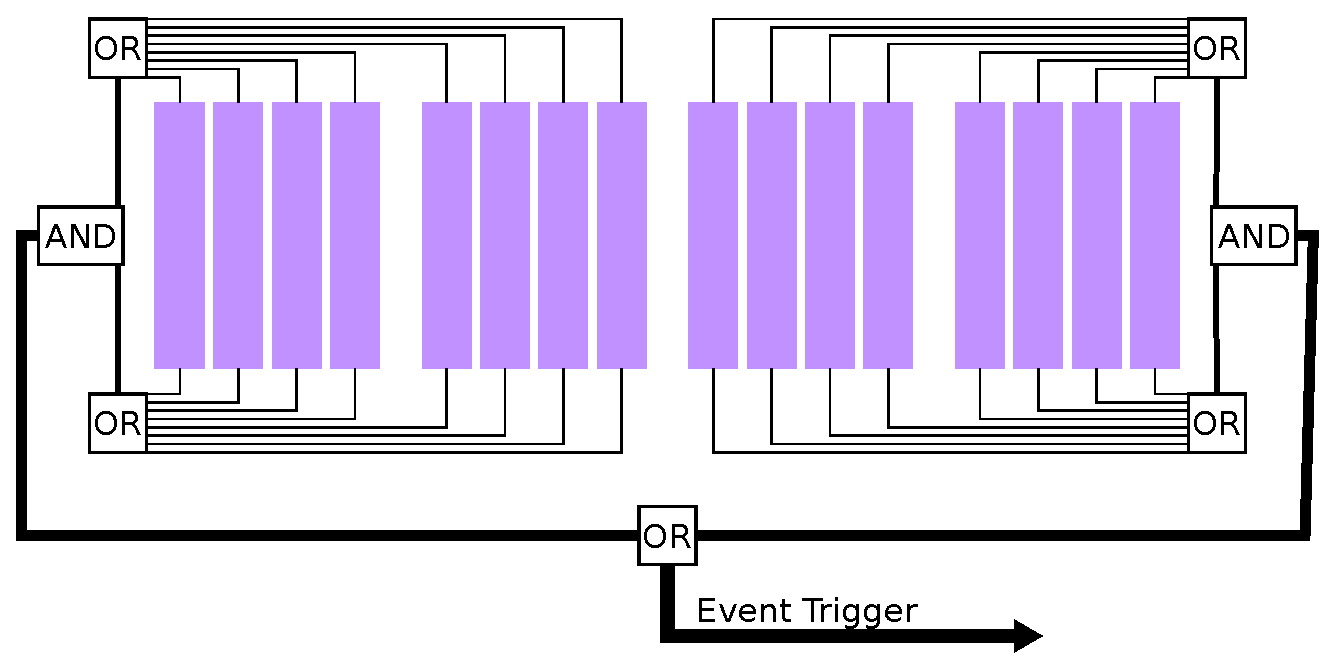
\includegraphics[width=1.0\textwidth]{figures/event_trigger.eps}
\label{fig:eventTrig}
\caption{The event trigger for the DAQ requires a coincidence between a top PMT and a bottom PMT from the same group of eight detectors.}
\end{figure}


\section{Setup}
\begin{comment}
Flight path and time resolution as a function of neutron energy - apply this to Ge ground and first excited state!
Beam monitor
Dead time
Include a sample calculation?  Like: this is what we see in the detector.  To get an absolute cross-section, here is the calculation:
counts * time * particle current * target thickness
So we get the counts this way and the time with the signal from the DAQ and the target thickness from Hope
\end{comment}

The time resolution of the TOF spectrum is limited by the time spread of the beam bunch and is approximately 1.5 ns.  A 16 MeV \He{3} can populate many excited states in \GeTargets; the energy difference between the ground and first excited state, together with the time resolution, determines the minimum flight path.

% figure: \Ge{76}, 74Ge level scheme

Conservation of energy and momentum determines the time $t$ it takes for a neutron with relativistic momentum $p$ to travel the distance $d$ between the target and the detector.

\begin{equation}
t(p) = \frac{d}{v} = d\times\sqrt{\frac{m^2+p^2/c^2}{p^2}}
\label{eq:TOF2}
\end{equation}


Requiring a separation between the ground state and first excited state of \Ge{76} that is greater than or equal to the time resolution,

\begin{equation}
d = \Delta t/v = 1.5 ns / v \sim 15 m
\label{eq:requiredDist}
\end{equation}

The room is too small for this flight path; the largest it can accomodate is 14.6 m, so cleanly separating the ground state from the first excited state will be difficult in \GeTargets.

The absolute cross section is the number of times a reaction occurred normalized by the total number of particles incident on the target and the number density of nuclei in the target:

\begin{equation}
\text{cross section} = \frac{\text{times reaction occurred}}{\text{particles incident on target} \times \text{number density of target nuclei}}

\text{cross section} = \frac{\text{times reaction occurred}}{\text{particle current} \times \text{time} \times \text{target thickness}}
\label{eq:cross_section}
\end{equation}

How many reactions occured and the target thickness do not affect the setup of the detector.  Calculating the number of reactions requires the efficiency of the detector.  Chapter ?? discusses this in detail.  The efficiency is approximately 3\% for all bars.  The target thickness is well-known from RBS measurements; the results are summarized in Chapter ?? and a description of the analysis is in Appendix ??.  Maintaining good energy resolution does dictate a target choice, however.  Because the \Ge{76} targets are too thin to be self-supporting, they are backed by a gold foil.  The target is positioned so that the first material the beam encounters is Ge.  Resulting neutrons can pass through the gold without the energy straggling that would afflict the \He{3} were it to pass through the gold.

The need for accurate time and particle current both affect the experimental setup.  The DAQ provides a 100 Hz NIM logic pulse, providing a measure of time.  But the DAQ cannot collect new events while it is processing an event.  A measure of the time experienced by the DAQ is the appropriate time to use when calculating the cross section.  In addition to a 100 Hz signal, the DAQ also provides a NIM logic pulse that is low when the DAQ is busy.  Vetoing the timing signal with this busy signal gives the live time needed for the cross section calculation.  The schematic is shown in figure ??.

There are several ways to record information about the particle current.  The most reliable is to measure RBS from the gold backing with a Silicon detector.  Because the \Mg{26} target is self-supporting, it is necessary to record other measures, such as the charge collected on the beamstop and the gamma reaction to a small NaI2 crystal, both of which show a linear relationship with the beam current within statistical error.

% figure: Si, Q.live, NaI accumulation

% figure: full electronics

\subsection{Testing with 26Mg}
\begin{comment}
Show results from first run and look at timing - hey it's all right!
Look at background - will need to improve
\end{comment}

\GeTargets cross-sections are predicted to be 300 mb, much lower than previous cross-sections measured with the neutron wall.  \Mg{26} has a cross-section of ?? mb and its differential cross-section (right word?) has been well measured by ?? [CITE!].  Since its level structure is similar to \GeTargets in that is has a low-lying 0+ first excited state, \Mg{26}(\He{3},n) serves as an excellent system to test the neutron wall.

% figure: 26Mg level scheme (along with Ge level scheme?)

The TOF spectrum at the forwardmost angle is shown in Figure ??.  The neutron peak has a width of 1.2 ns and is clearly visible against the background.  Figure ?? shows the agreement of the extracted cross-section to previously measured data.

% figure: Bar A TOF spectrum

% figure: 26Mg cross-section compared to old data

The concerning thing about this data is that the neutron peaks at angles with low cross-sections do not stand significantly above the random background.  This has serious implications for the \GeTargets experiment, where the cross-section is suspected to be even lower.  Current data on two-proton transfer typically has errors no worse than 20\%; to achieve such errors it is necessary to either reduce the background or increase the beam current.  Increasing the beam current substantially was not feasable because of ion source limitations.  The background comes primarily from low-energy $\gammaa$ radiation from the cement in the room and from muons produced by cosmic rays.  The next chapter discusses the construction of a cosmic-ray veto.

% % uncomment the following lines,
% if using chapter-wise bibliography
%
% \bibliographystyle{ndnatbib}
% \bibliography{example}




%
% Chapter 4
%

%
% Modified by Sameer Vijay
% Last Change: Wed Jul 27 2005 13:00 CEST
%
%%%%%%%%%%%%%%%%%%%%%%%%%%%%%%%%%%%%%%%%%%%%%%%%%%%%%%%%%%%%%%%%%%%%%%%%
%
% Sample Notre Dame Thesis/Dissertation
% Using Donald Peterson's ndthesis classfile
%
% Written by Jeff Squyres and Don Peterson
%
% Provided by the Information Technology Committee of
%   the Graduate Student Union
%   http://www.gsu.nd.edu/
%
% Nothing in this document is serious except the format.  :-)
%
% If you have any suggestions, comments, questions, please send e-mail
% to: ndthesis@gsu.nd.edu
%
%%%%%%%%%%%%%%%%%%%%%%%%%%%%%%%%%%%%%%%%%%%%%%%%%%%%%%%%%%%%%%%%%%%%%%%%

%
% Chapter 4
%

\chapter{MUON VETO DEVELOPMENT}
\label{chap:muVeto}
\begin{comment}
Explain some cosmic ray basics - only the stuff relevant to our detector (1 muon per square foot per second and MIP -> landau energy distribution).
Discuss materials available for veto and basic design decision of WLS
\end{comment}

\section{Testing with \MgReaction}
\begin{comment}
Show results from first run and look at timing - hey it's all right!
Look at background - will need to improve
\end{comment}

\GeTargets cross-sections are predicted to be much lower than previous cross-sections measured with the neutron wall.  The differential cross-section of \MgReaction, however, is on the order of 1~mb/sr and and has been well measured by \cite{Bohne_Mg}, making \Mg{26} a good candidate for testing the neutron wall.  The TOF spectrum at the forwardmost angle, 6$^{\circ}$, is shown in {\fig}~\ref{fig:MgTOF}.  The neutron peak has a width of 1.2 ns and is clearly visible against the background. 
% figure: Bar A TOF spectrum
\begin{figure}[htp]
%\centering
%\includegraphics[width=1.0\textwidth]{figures/MgTOF.eps}
\vspace{3in}
\caption{The 6$^{\circ}$ TOF spectrum for \MgReaction.}
\label{fig:MgTOF}
\end{figure}

The concerning thing about this data is that the neutron peaks at angles with low cross-sections do not stand significantly above the random background.  This has serious implications for the \GeTargets experiment, where DWBA calculations predict the cross-section to be $\sim$300~$\mu$b/sr.  Achieving 20\% uncertainty on the ground-state cross section requires either reducing the background or increasing the beam current.  Increasing the beam current was not feasible because of ion source limitations.  The background comes primarily from low-energy $\gamma$ radiation from the cement in the room and from muons produced by cosmic rays.  Neither vetoing nor shielding against $\gamma$-radiation would be effective since materials with high $\gamma$ interaction rates would also scatter incoming neutrons.  The muons, however, are charged and can be readily identified by their high interaction rate with nearly any material.  We therefore seek to reduce the muon component of the random background.

A practical solution to the muon background is to make a veto shield that registers the likely presence of a muon.  The events identified as muon events can then be discarded.  Distinguishing between muons and non-charged particle interactions using additional scintillator material is possible because of the difference in likelihood of interaction.  
\begin{figure}[hp]
\centering
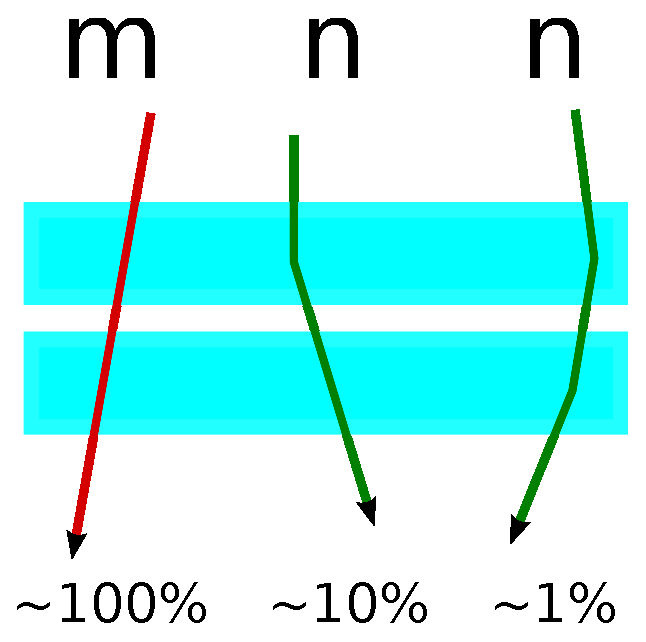
\includegraphics[width=0.4\textwidth]{figures/simpleVeto.eps}
\caption{The charged muon has a nearly 100\% chance of leaving a detectable signal in both scintillators, while the neutron, lacking charge, is much less likely to interact in even one of the scintillators.  The likelihood of detecting a neutron interaction depends on both the thickness of the scintillator and the threshold of the detector; for a 5 cm thick scintillator with a threshold at approximately the Th edge, the likelihood of detecting a 20 MeV neutron is about 10\%.}
\label{fig:simpleVeto}
\end{figure}
The energy distribution of muons incident on the neutron detector peaks at 100 GeV/C \cite{PDG}, so that most of the muons traveling through the detector are Minimum Ionizing Particles (MIP's).  This means that their energy loss is proportional to their path length in that material.  Muons at these energies deposit 1 MeV/cm2/g \cite{PDG}.  The detector consists of plastic with a density of ??, so the muons can deposit between 0.5 MeV to 80 MeV depending on their path through the plastic.  While the charged muon will trigger both detectors provided its path deposits energy above the detector threshold, the neutron is highly unlikely even to interact in both detectors.  The bars of the neutron detector are 5 cm thick; the chance of detecting a 20 MeV neutron when the detection threshold is at approximately the Th edge is 10\%, making the chance of a neutron interacting in two bars only 1\%.  If the muon veto is made of a thinner bar of scintillator, the probability of a detectable neutron interaction in both drops further.  By placing a thin ($\sim$1 cm) scintillator over the neutron detector bar, it is possible to identify muons to an accuracy of at least 99\%.  Note that such a veto does not identify $\gamma$ radiation because it has an efficiency similar to neutrons in BC408.

\section{Light Collection with WLS}
\begin{comment}
Describe light collection with WLS
Explain why we loop the WLS and collect light from both ends
Discuss the light limitations of light guides (Liouville) and ways to increase light collection with WLS (more!)
Describe fragility of WLS, how some efforts make custom plastic clamps to make it robust, how this doesn't work for you so you made a break and attached a cable.  Discuss signal loss.
\end{comment}
The scintillator bars of the neutron detector are outfitted with two PMT's, each coupled to its end via a non-scintillating light guide.  Having two PMT's is essential both for good timing information and also to lessen the position sensitivity of the signal.  Instrumenting the veto scintillators in this way was not feasible.  Fitting a top and bottom PMT to each veto bar would require 32 PMT's and lightguides, along with independent power supplies for each.  Instead, wavelength-shifting fiber (WLS) was chosen to collect the light.

WLS collects light by absorbing broad-spectrum radiation and re-emitting that light in the green.  It is possible to coat the fiber with material with an index of refraction that guarantees total internal reflection for green light, and so the light bounces in the fiber until it reaches a detector.  WLS largely eliminates position sensitivity because it can be arranged on the detector so that no part is distant from the collecting fiber [cite??].  Because the fiber is fairly flexible, its pattern on the detector can be designed so that the fiber exits the plastic in a single bundle, allowing instrumentation with only one PMT.

Possible disadvantages to WLS are signal intensity [cite??] and fragility of the fiber.  Sufficient light intensity to boost the signal above the noise is a serious concern, and can be overcome by using many WLS strands to collect light [cite NASA].  The fragility of the WLS is more difficult to remedy.  To maximize light collection, the fiber on the detector should bee taken directly to the PMT, which should be as close to the plastic as possible to minimize signal attenuation.  In some designs [CITE!], this is acheived by enclosing the fiber run to the PMT in a stiff cast.  The design for the neutron wall needed flexibility in PMT placement, making a fixed support between the detector and PMT impractical.  Several attempts were made to run the WLS collection fiber directly from the scintillator to the PMT, but even with careful handling, the fiber quickly degraded and eventually snapped.  Such degredation would have left no way to access the veto's signals and was unacceptable.  The decision was made to sever the WLS at the end of the plastic and make a robust cable to attach to the WLS and carry the signal to the PMT.  While severing the WLS causes significant light loss, it ensures durability.  The details of this design are discussed in the next section.  

\section{Paddle Design}
\begin{comment}
Schematics
Tolerances
Making sure the transmit cable lines up with the paddle WLS fibers!  Dowels.  Tolerance doesn't actually need to be that good
connecting cable with PMT
cable design - hosing for protection
\end{comment}

The main components of a veto paddle are the scintillator and WLS, which does the actual detection, the endpiece that glues onto the scintillator, which fixes the position of the WLS coming off the scintillator, and the cable, which connects to the WLS and carries the signal to the PMT.  Each piece is discussed in this section.

The scintillator material itself is $\sim3/8$'', thinner than the bars of the neutron detector.  This is desirable because we don't want the neutrons to interact with material other than the neutron detector, but the thin material can still be efficient at detecting muons.  The fiber is glued to the paddle in a ``U'' shape as in {\fig}~\ref{fig:paddle}.  This is done to maximize light collection.  Light absorbed by the fiber propagates in both directions along the fiber axis; if one end of the fiber terminates, the light must reflect off the surface and travel back to the PMT, and light loss occurs both at the reflection and there's attenuation along the path.  Light loss at the terminating surface can be lessened somewhat with the application of reflective paint [CITE] and more so by silvering the surface [CITE], but a simpler method of recovering the light is to loop the fiber on the scintillator so that both ends can terminate at the PMT, allowing collection of light regardless of its travel direction.  With such a design, care must be taken to avoid extreme bending of the WLS, as it is easily damaged.  The bend radius chosen was ?? cm, which seemed to have no adverse effect on the WLS.
\begin{figure}[htp]
\centering
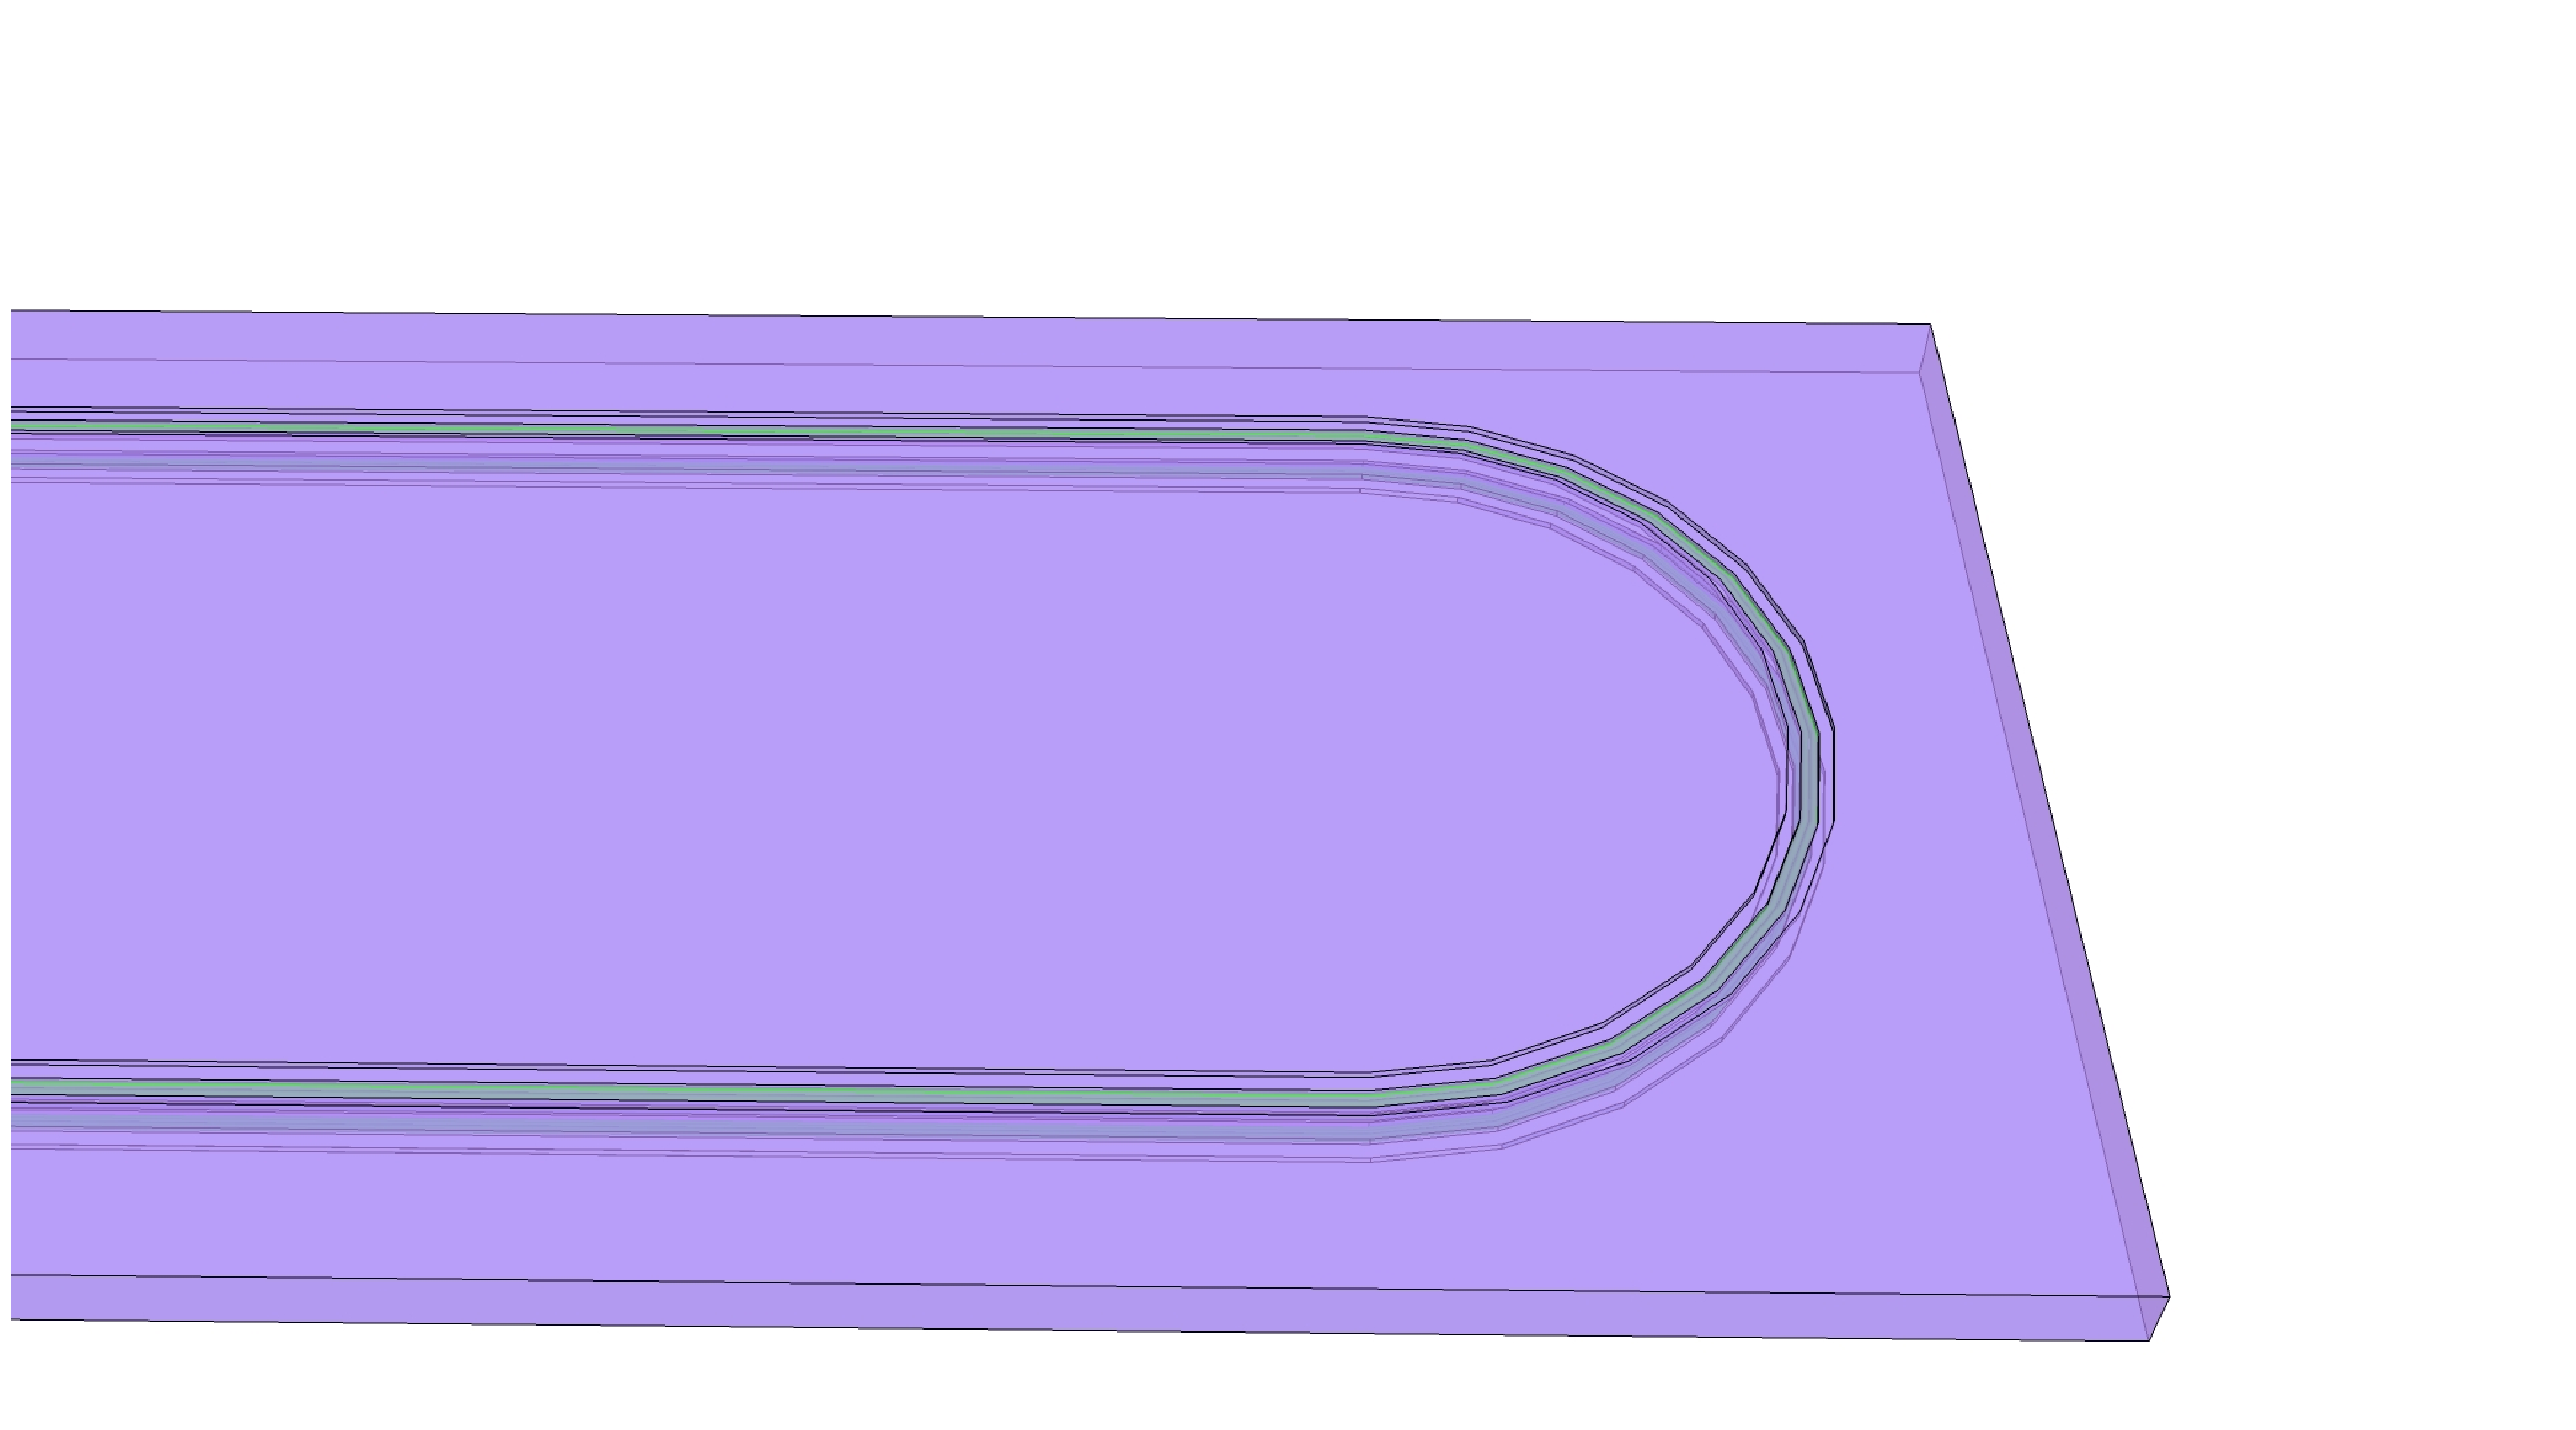
\includegraphics[width=0.5\textwidth]{figures/veto_end.eps}
\caption{The WLS is glued to the scintillator in a ``U'' shape to maximize light recovery.}
\label{fig:paddle}
\end{figure}


In general, the design goal was to maximize light collection while ensuring durability.  We could see that occasionally there was a default in the WLS cladding and were concerned that some fiber would suffer from more light loss than others.  The solution, using multiple strands of fiber to collect light, was intended to buffer the detector from chance defects in the WLS.  Using multiple strands of fiber also increases light collection, as found in [CITE!].  In general, light collection increases as more WLS is added to the surface, and there is not noticable position sensitivity if no part of the scintillator material is more than $\sim$5~cm from WLS fiber.  While more fiber could have been added to the surface of the scintillator, it already covered the surface and provided sufficient signal, shown in {\fig}~\ref{fig:vetoSignal}.  Furthermore, the WLS was glued into a channel machined into the scintillator to keep it from being damaged.  While more WLS fiber could increase the light collection, increasing the fiber on the surface would have meant machining away more scintillating material.  We did not want to reduce the possible energy deposition of the muons, as this was already quite low due to the thinness of the scintillator.
\begin{figure}[htp]
\centering
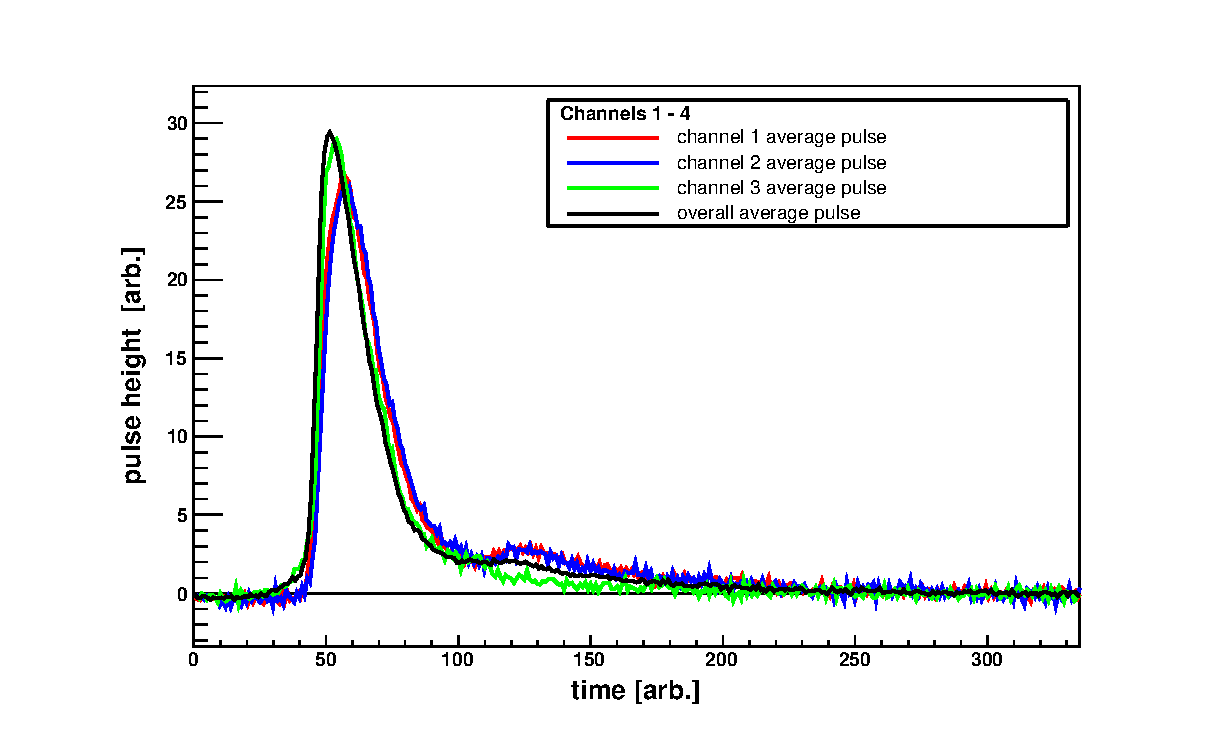
\includegraphics[width=0.5\textwidth]{figures/PulseChan_1_4.eps}
\caption{Pulses from muons in the veto paddles.}
\label{fig:vetoSignal}
\end{figure}


An endcap fitted to the scintillator helps protect the WLS and also ensures the WLS location, allowing good alignment to the fibers in the cable.  The endcap minimizes possible WLS flexing by connecting to machined indents in the scintillator with a press fit.  Because the endcap extends into the scintillator, bending the fiber perpendicular to its axis is essentially eliminated.  Scintillator is also machined away from the fiber's entrance to the endcap to avoid point pressure.  Once the endcap is slid onto the scintillator, it is glued in place, not to secure it to the scintillator, but to fix the WLS in their holes completely so that the surface of the endcap can be polished without damaging the WLS.

The cable that transmits the light from the WLS to the PMT has three seperate parts.  A connector mates with the endcap attached to the scintillator and connects to the tubing, which is 2~m long and connects to a connector that attaches to the PMT.  At each interface between tubing and connector, the primary concern is that the stresses on the transmission fiber be small enough to not damage the fiber.  A hose barb attached to each connector allows the transmission fiber through and also allows the tubing to firmly connect without putting strin on the fiber.  Slightly stiff tubing (durometer rating = ??) was chosen to help limit the bend radius of the cable, further protecting the transmission fiber.  
\begin{figure}[htp]
\centering
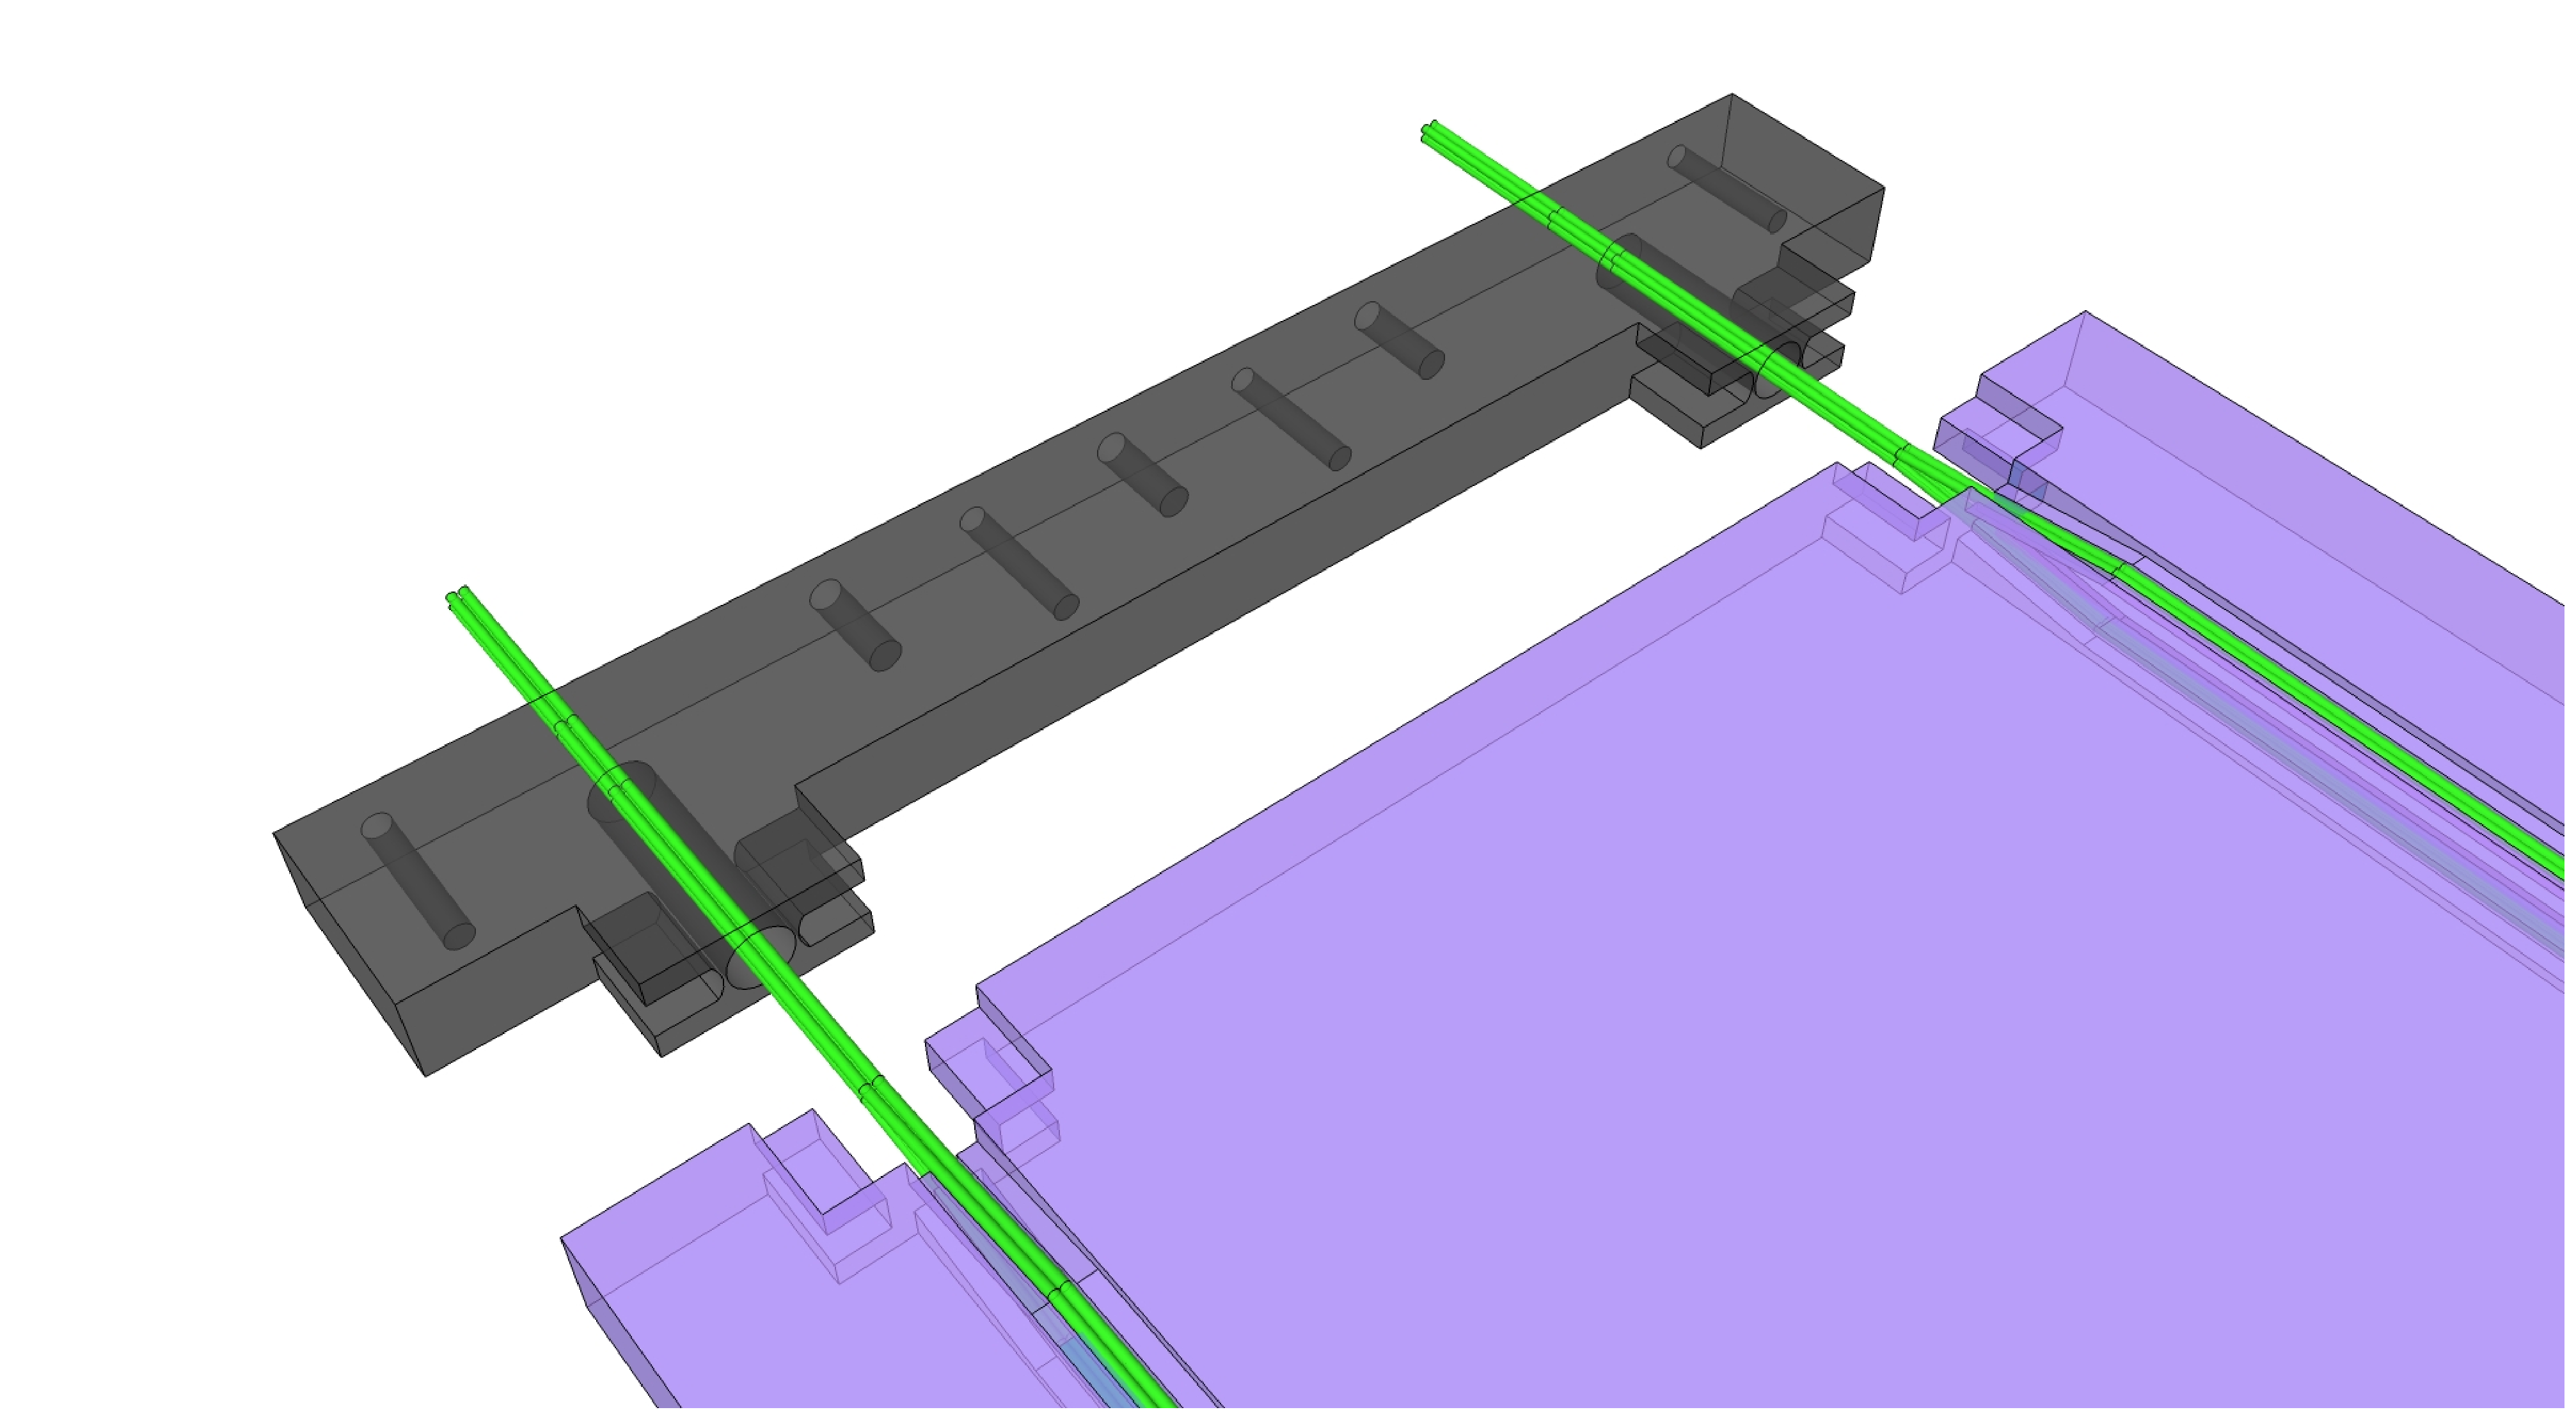
\includegraphics[width=1.0\textwidth]{figures/veto_assembly.eps}
\caption{The endcap will be glued to the scintillator after it is slid into place.}
\label{fig:paddleAssembly}
\end{figure}

The primary concern for the portion of the cable that attaches to the endcap is that each transmission fiber completely overlap its WLS fiber.  The diameter of the transmission fiber is ??~mm, larger than the ??~mm-diameter WLS fiber, which allows misalignment of ??~mm without greatly impacting light collection.  Tight-fitting dowels help align the region of the cables containing the fiber cluster.  This is particularly important because the connectors are machined from plastic and are not perfectly square - some connectors bow as much as 20 mils from normal.  The only regions that must be carefully aligned, however, are the fiber clusters, and the dowels constrain these regions to less than ?? mils, ensuring an alignment of ?? mm.
\begin{figure}[htp]
\centering
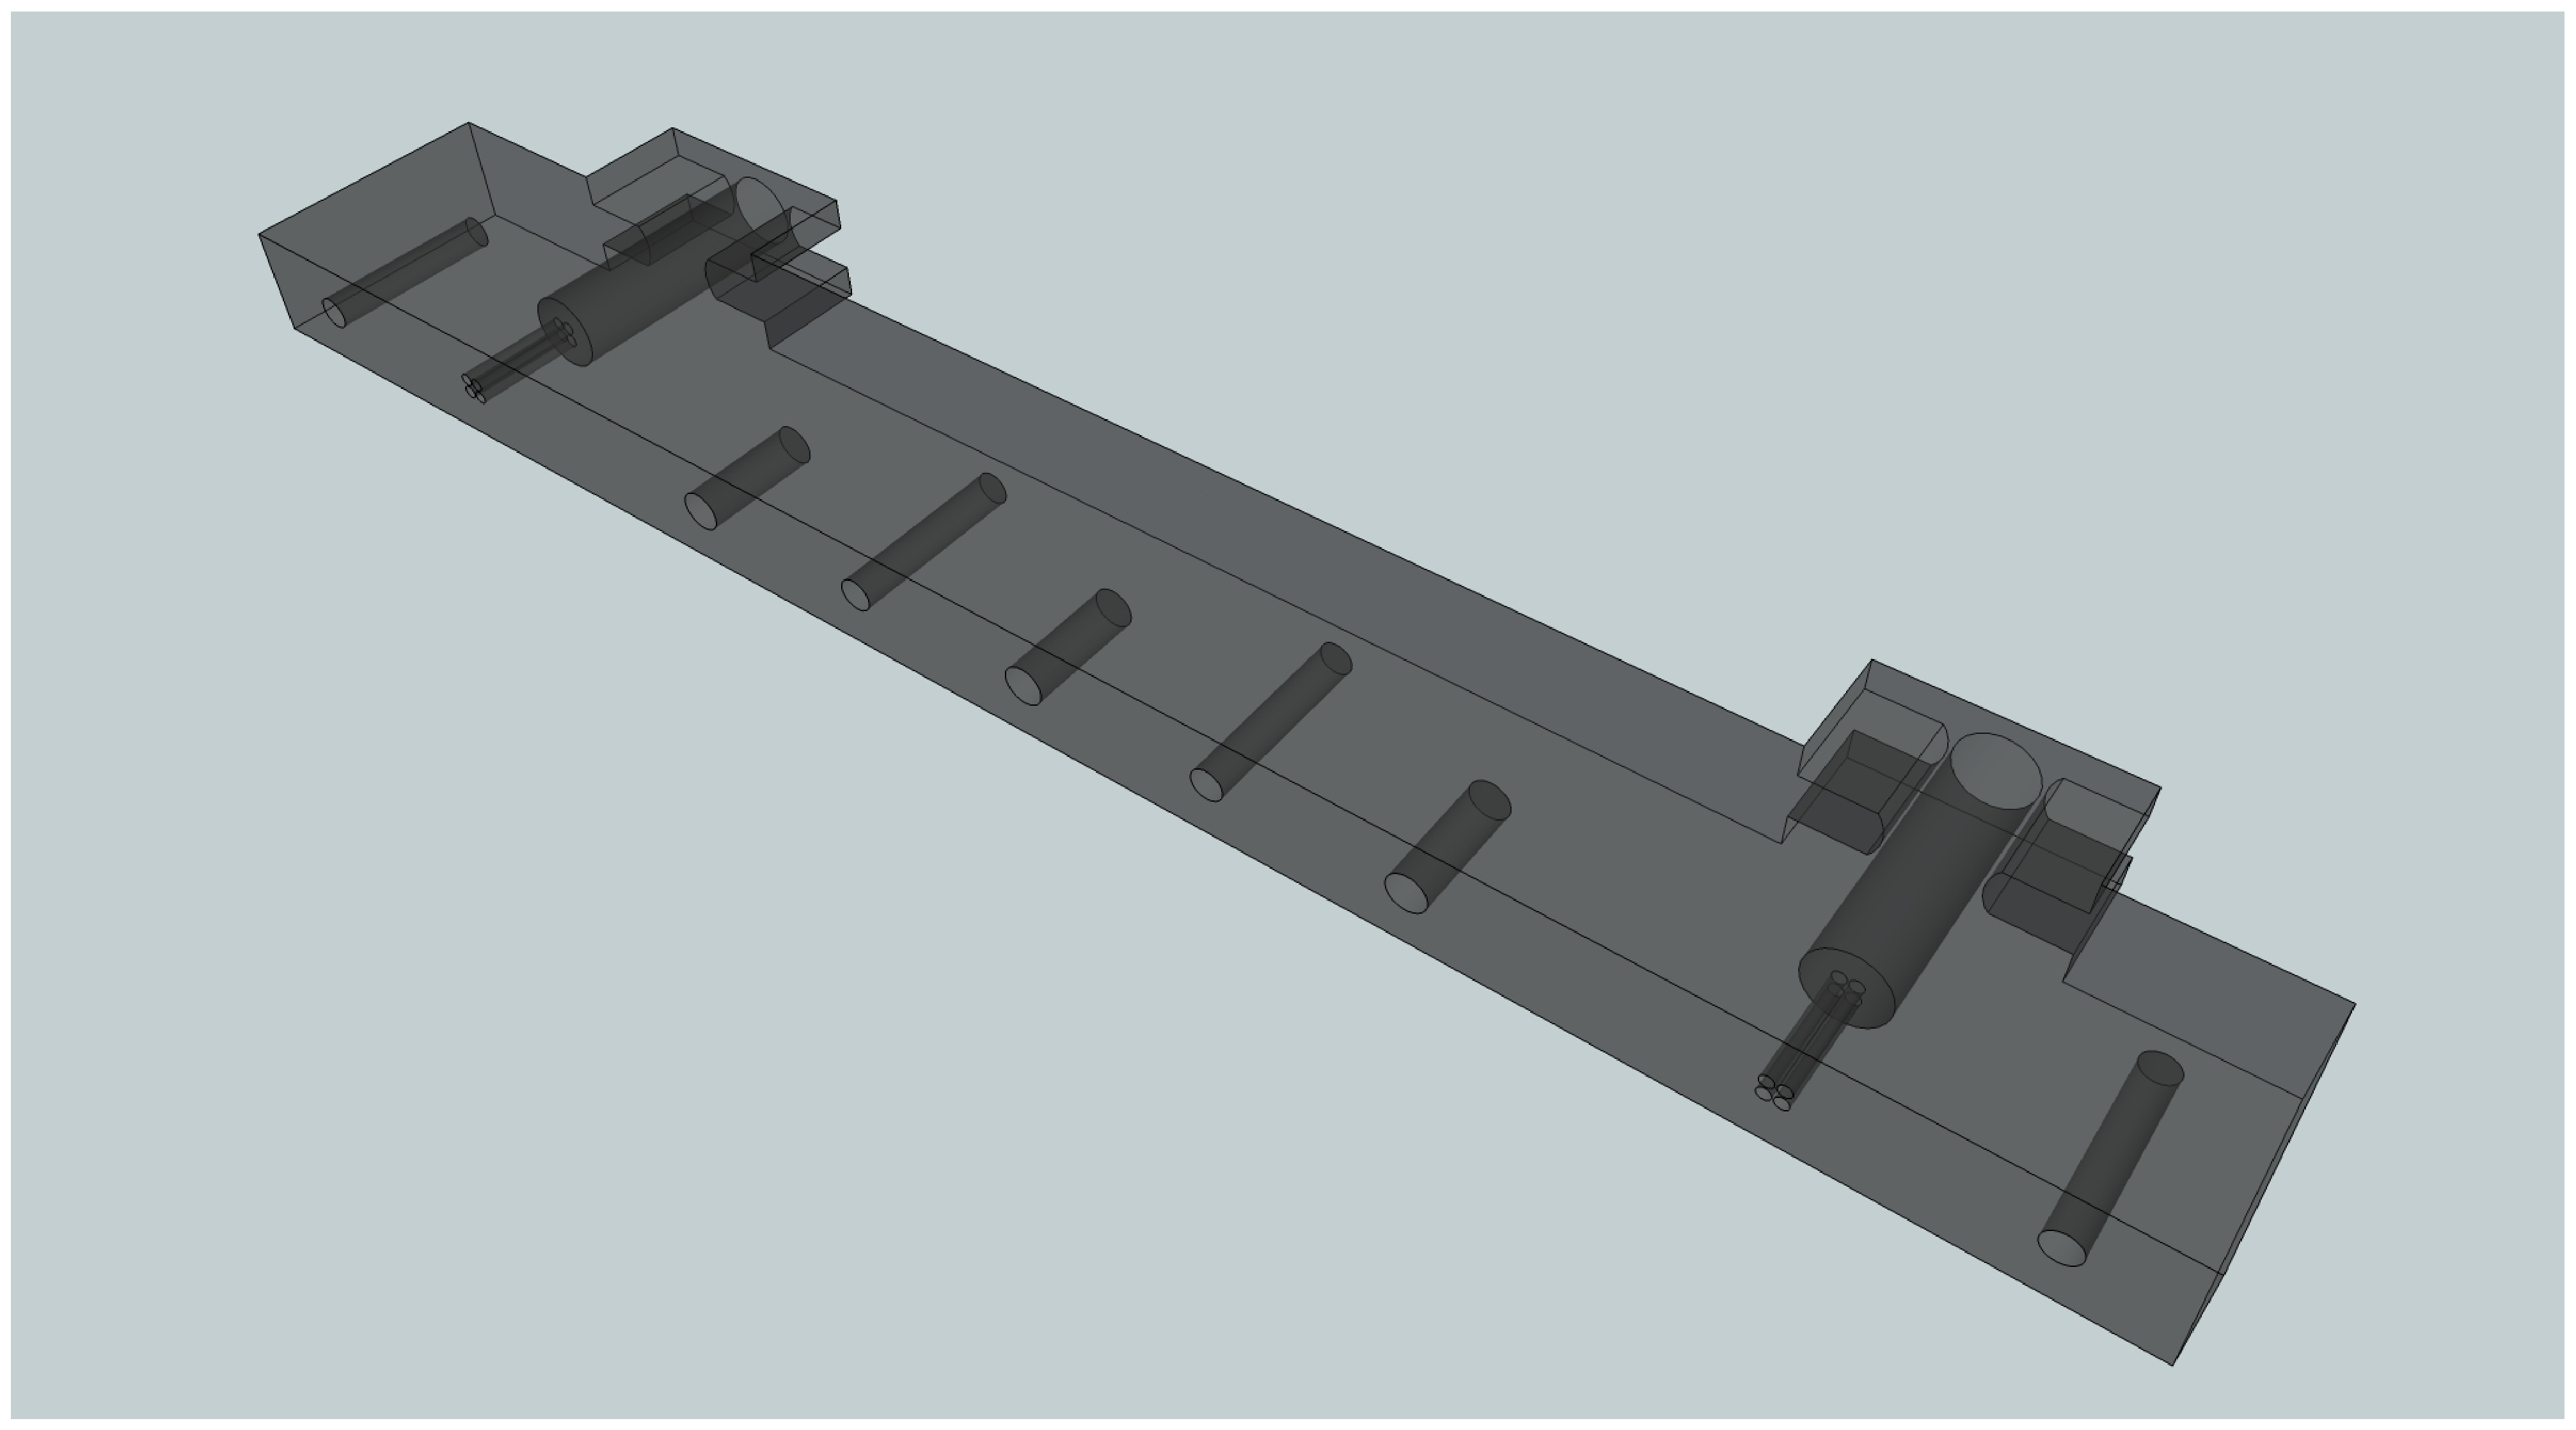
\includegraphics[width=1.0\textwidth]{figures/paddle_connector.eps}
\caption{The cable connector must align with the WLS on the endcap.}
\label{fig:paddleAssembly}
\end{figure}


\section{Paddle Performance}
\label{sec:singleVeto}

%\subsection{tests on intrinsic efficiency}
\begin{comment}
Show signal from detector
Talk about first tests?  Can talk about sensitivity to geometric alignment of trigger paddles ...
Maybe mention this and then be like, ``this is why we decided to look at the efficiency this other way that was less sensitive''
except you weren't able to do further tests so you'll just have to say the limits you got
\end{comment}
The intrinsic efficiency of the paddles can be tested by requiring a coincidence with several paddles.  The several-detector coincidence identifies signals as muons.  If the coincidence paddles are arranged so that the path of any muon intersecting all the veto paddles must also intersect the volume of the veto paddle, the efficiency measured is the veto's intrinsic efficiency, separated from its geometric coverage of whatever detector it is vetoing.

In practice, arranging the available scintillator to force muons through the test volume was difficult because the available scintillator was instrumented with bulky lightguides and could not be laid directly on the test volume.  A simple cosmic ray simulation program helped determine an arrangement that maximized geometrical efficiency.  This arrangement, however, was extremely sensitive to placement; measured efficiency of the same bar could change from 98\% to 75\% with a displacement of a few centimeters.
\begin{figure}[htp]
\centering
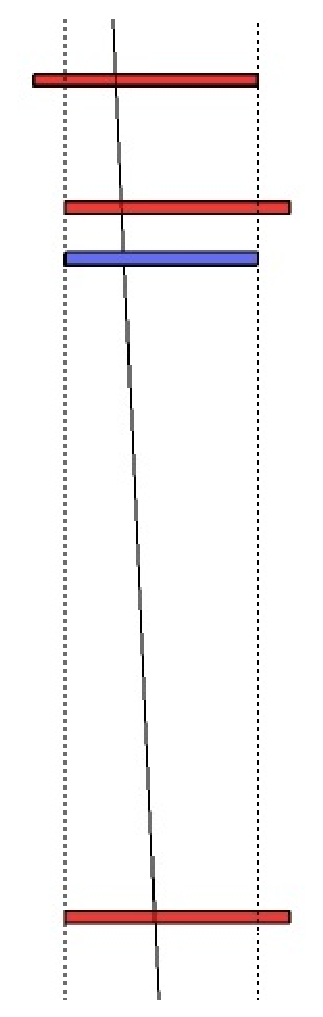
\includegraphics[width=1.0\textwidth]{figures/veto_test_layout.eps}
\caption{This arrangement of coincidence material ensures that muons triggering all coincidence detectors must also travel through the veto paddle.  The coincidence material is drawn in red while the veto paddle is in blue.}
\label{fig:efficiencyTest}
\end{figure}

The efficiency was measured by counting how often the veto paddle had a detectable signal when all the coincidence material registered a coincidence.  Assuming the muon was constrained to travel through the veto paddle volume, the ratio gives the efficiency.  The DAQ Event signal was a logic pulse resulting from the coincidence of the coincidence paddles.  This logic pulse also acted as a Start for a TAC.  The TAC stop signal was a delayed, discriminated veto paddle signal.  The outgoing TAC signal was sent to an analog to digital converter (ADC) for integration.  Signals from the veto paddle coincident with the other scintillators show up in the timing spectrum as a peak at the time of the delay.  The integral of this timing peak divided by the number of event triggers gives the efficiency.
% figure: the considerably complicated spectrum
\begin{figure}[htp]
\centering
\subfloat[][]{
   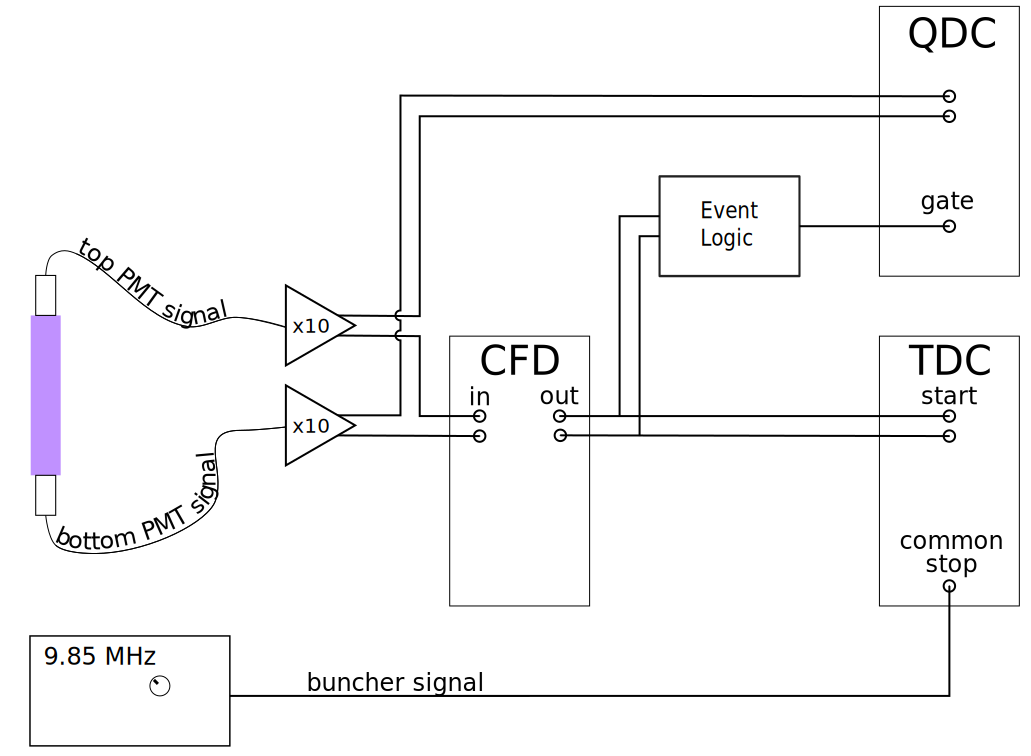
\includegraphics[width=0.45\textwidth]{figures/vetoTest_electronics.eps}	
}
\subfloat[][]{
	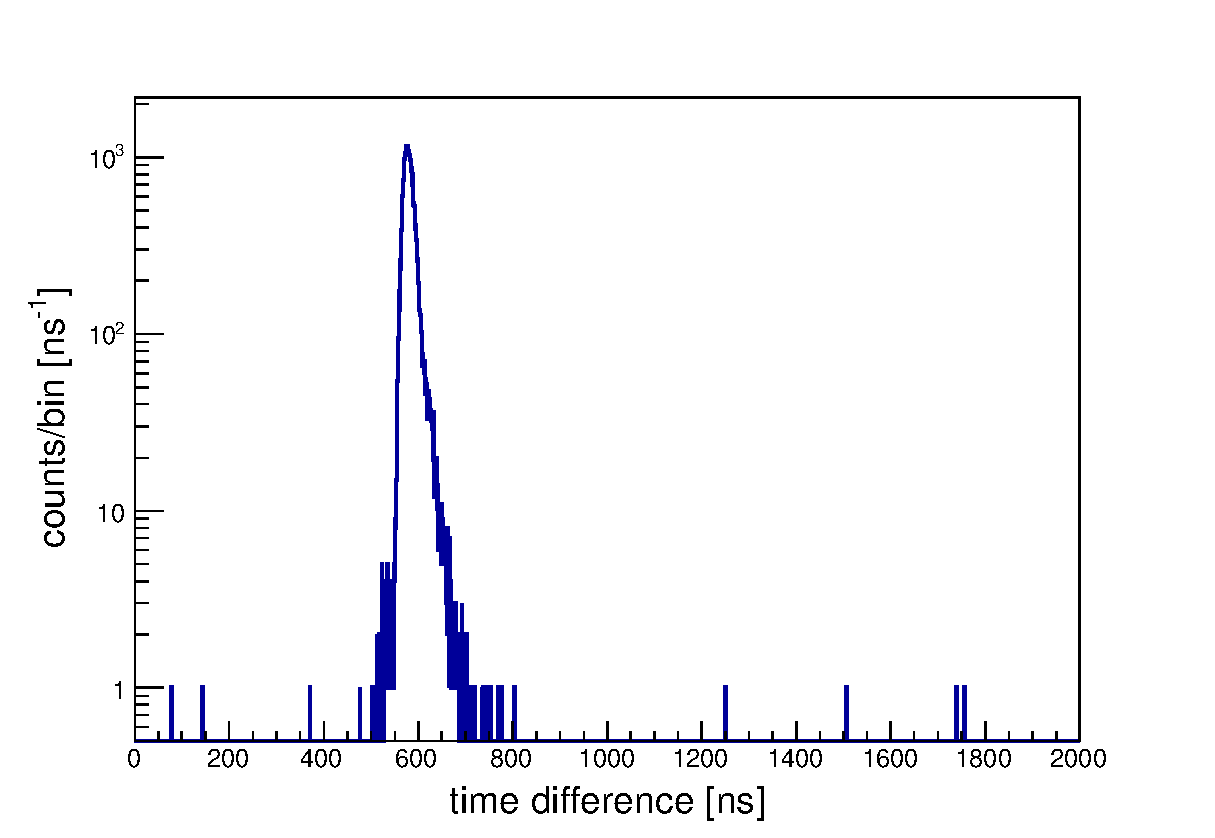
\includegraphics[width=0.45\textwidth]{figures/efficiencyTest_timingSpectrum.eps}
}
\caption{The location of the timing peak is set by the delay introduced to the discriminated veto paddle signal.  Integrating the timing peak gives the number of muons that generated an observable signal in the veto paddle.}
\label{fig:vetoTestElectronics}
\end{figure}

Testing the efficiency of the veto paddle with this setup was not ideal because the geometrical efficiency was very sensitive to the placement of the coincidence detectors; measured efficiency of the same bar could change from 98\% to 75\% when one of the coincidence detectors was shifted by as little as a few centimeters.  However, this setup was useful in testing the effect of the cable polishing, cable out-of-true-ness, and the condition of the plastic scintillator.  In general, all efficiency measurements fell between 94\% and 98\%: even the veto paddles made of the most badly damaged plastic were as efficient as the veto paddles made from the plastic in excellent condition.  No statistically significant differences were seen between cables with the most and the least amount of bowing.  Polishing the cables with the bull-nose single-crystal diamond increases detection efficiency by $\sim2$\%, although it should be noted that the change may have been due to correlated noise in the system rather than to improved light transmission.  The discriminator threshold, set to its lowest value, gave an efficiency of 98\% compared to 94\% when set to its highest value.

Testing the position dependence of the efficiency using the setup described above was not practical due to its sensitivity on positioning.  Instead, the response of the veto paddles to a loosely collimated $\gamma$ source was tested.  Counting detected $\gamma$ radiation showed a deviation of less than 8.5\% over the veto paddle.  While this is not a measurement of the position dependence of the muon efficiency, it does limit the efficiency change over the paddle since muons typically deposit at least double the energy of the $\gamma$ radiation from the $^{60}$Co source.  See {\fig}~\ref{fig:positionDependence} for the variation of the efficiencies.
\begin{figure}[htp]
\centering
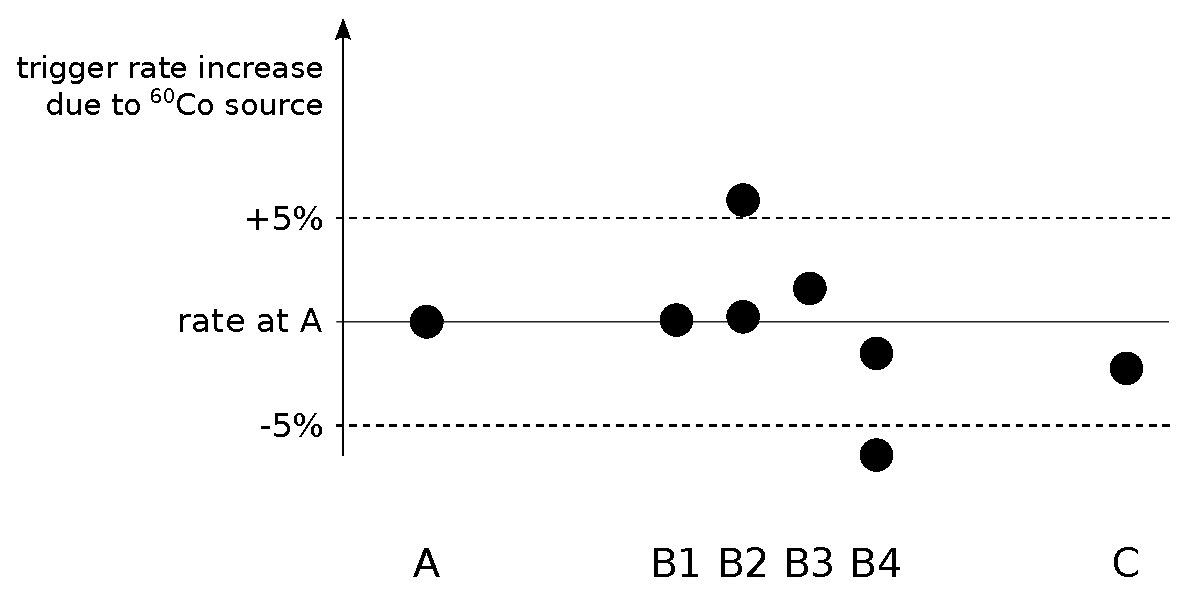
\includegraphics[width=1.0\textwidth]{figures/efficiency_positionDependence.eps}
\caption{The dependence of the number of detected events on the position of a loosely-collimated $^{60}$Co source.  Positions A and C are closest and furthest from the cable connection, respectively.  Position B is the center of the veto paddle.  Data was taken in the center across the bar to test for horizontal position dependence.  The spread is approximately 8.5\%.}
\label{fig:positionDependence}
\end{figure}


\subsection{On-Detector Efficiency}
\begin{comment}
Initial efficiency - would be nice to show this data
Describe different cosmics that hit the neutron bar but miss the veto - argh!
Discuss changes made to mounting to improve coverage - show new data (cosmics)
\end{comment}
Sixteen veto paddles were initially mounted on top of the neutron detector support structure to avoid removing (and potentially damaging) the heavy neutron detectors.  Each veto paddle was $\sim$2~cm offset from a bar in the neutron detector.  Running a test with \MgReaction showed good cosmic rejection in the two innermost bars of each four-bar unit and worse rejection in the outer two bars by about 20\%, corresponding to double the cosmic background.  The outer bars act as additional veto for the inner bars, while the outer bars enjoy no such additional vetoing.  
\begin{figure}[htp]
%\centering
%\includegraphics[width=1.0\textwidth]{figures/initialBackground.eps}
\vspace{3in}
\caption{Room background after rejection with the initial placement of the veto paddles.  Note that the high-background bars are those on the ends of each group of four.}
\label{fig:initialBackground}
\end{figure}

A simulation of the cosmic background indicated that the geometrical efficiency was very sensitive to the distance between the veto paddle and neutron detector bar as well as the distance between the bars of the neutron detector.   The bars in the neutron detector were moved as close as the mounting screws would allow, within 1~cm.  Instead of attaching the veto paddles on top of the retaining bars on the neutron detector, they were taped to the bars and both bar and veto paddle were supported together by the same retaining bar.  The separation between the bars of the neutron detector and their veto paddle is $\sim$0.5~cm due to stiff foam placed between the two to protect the WLS channels in the veto paddles.  Material was also added to the sides of the outermost neutron detectors.  The final setup is shown in {\fig}~\ref{fig:vetoSetup}.  These changes improved both the average and uniformity of the background rejection, as can be seen in {\fig}~\ref{fig:finalBackground}.
\begin{figure}[htp]
\centering
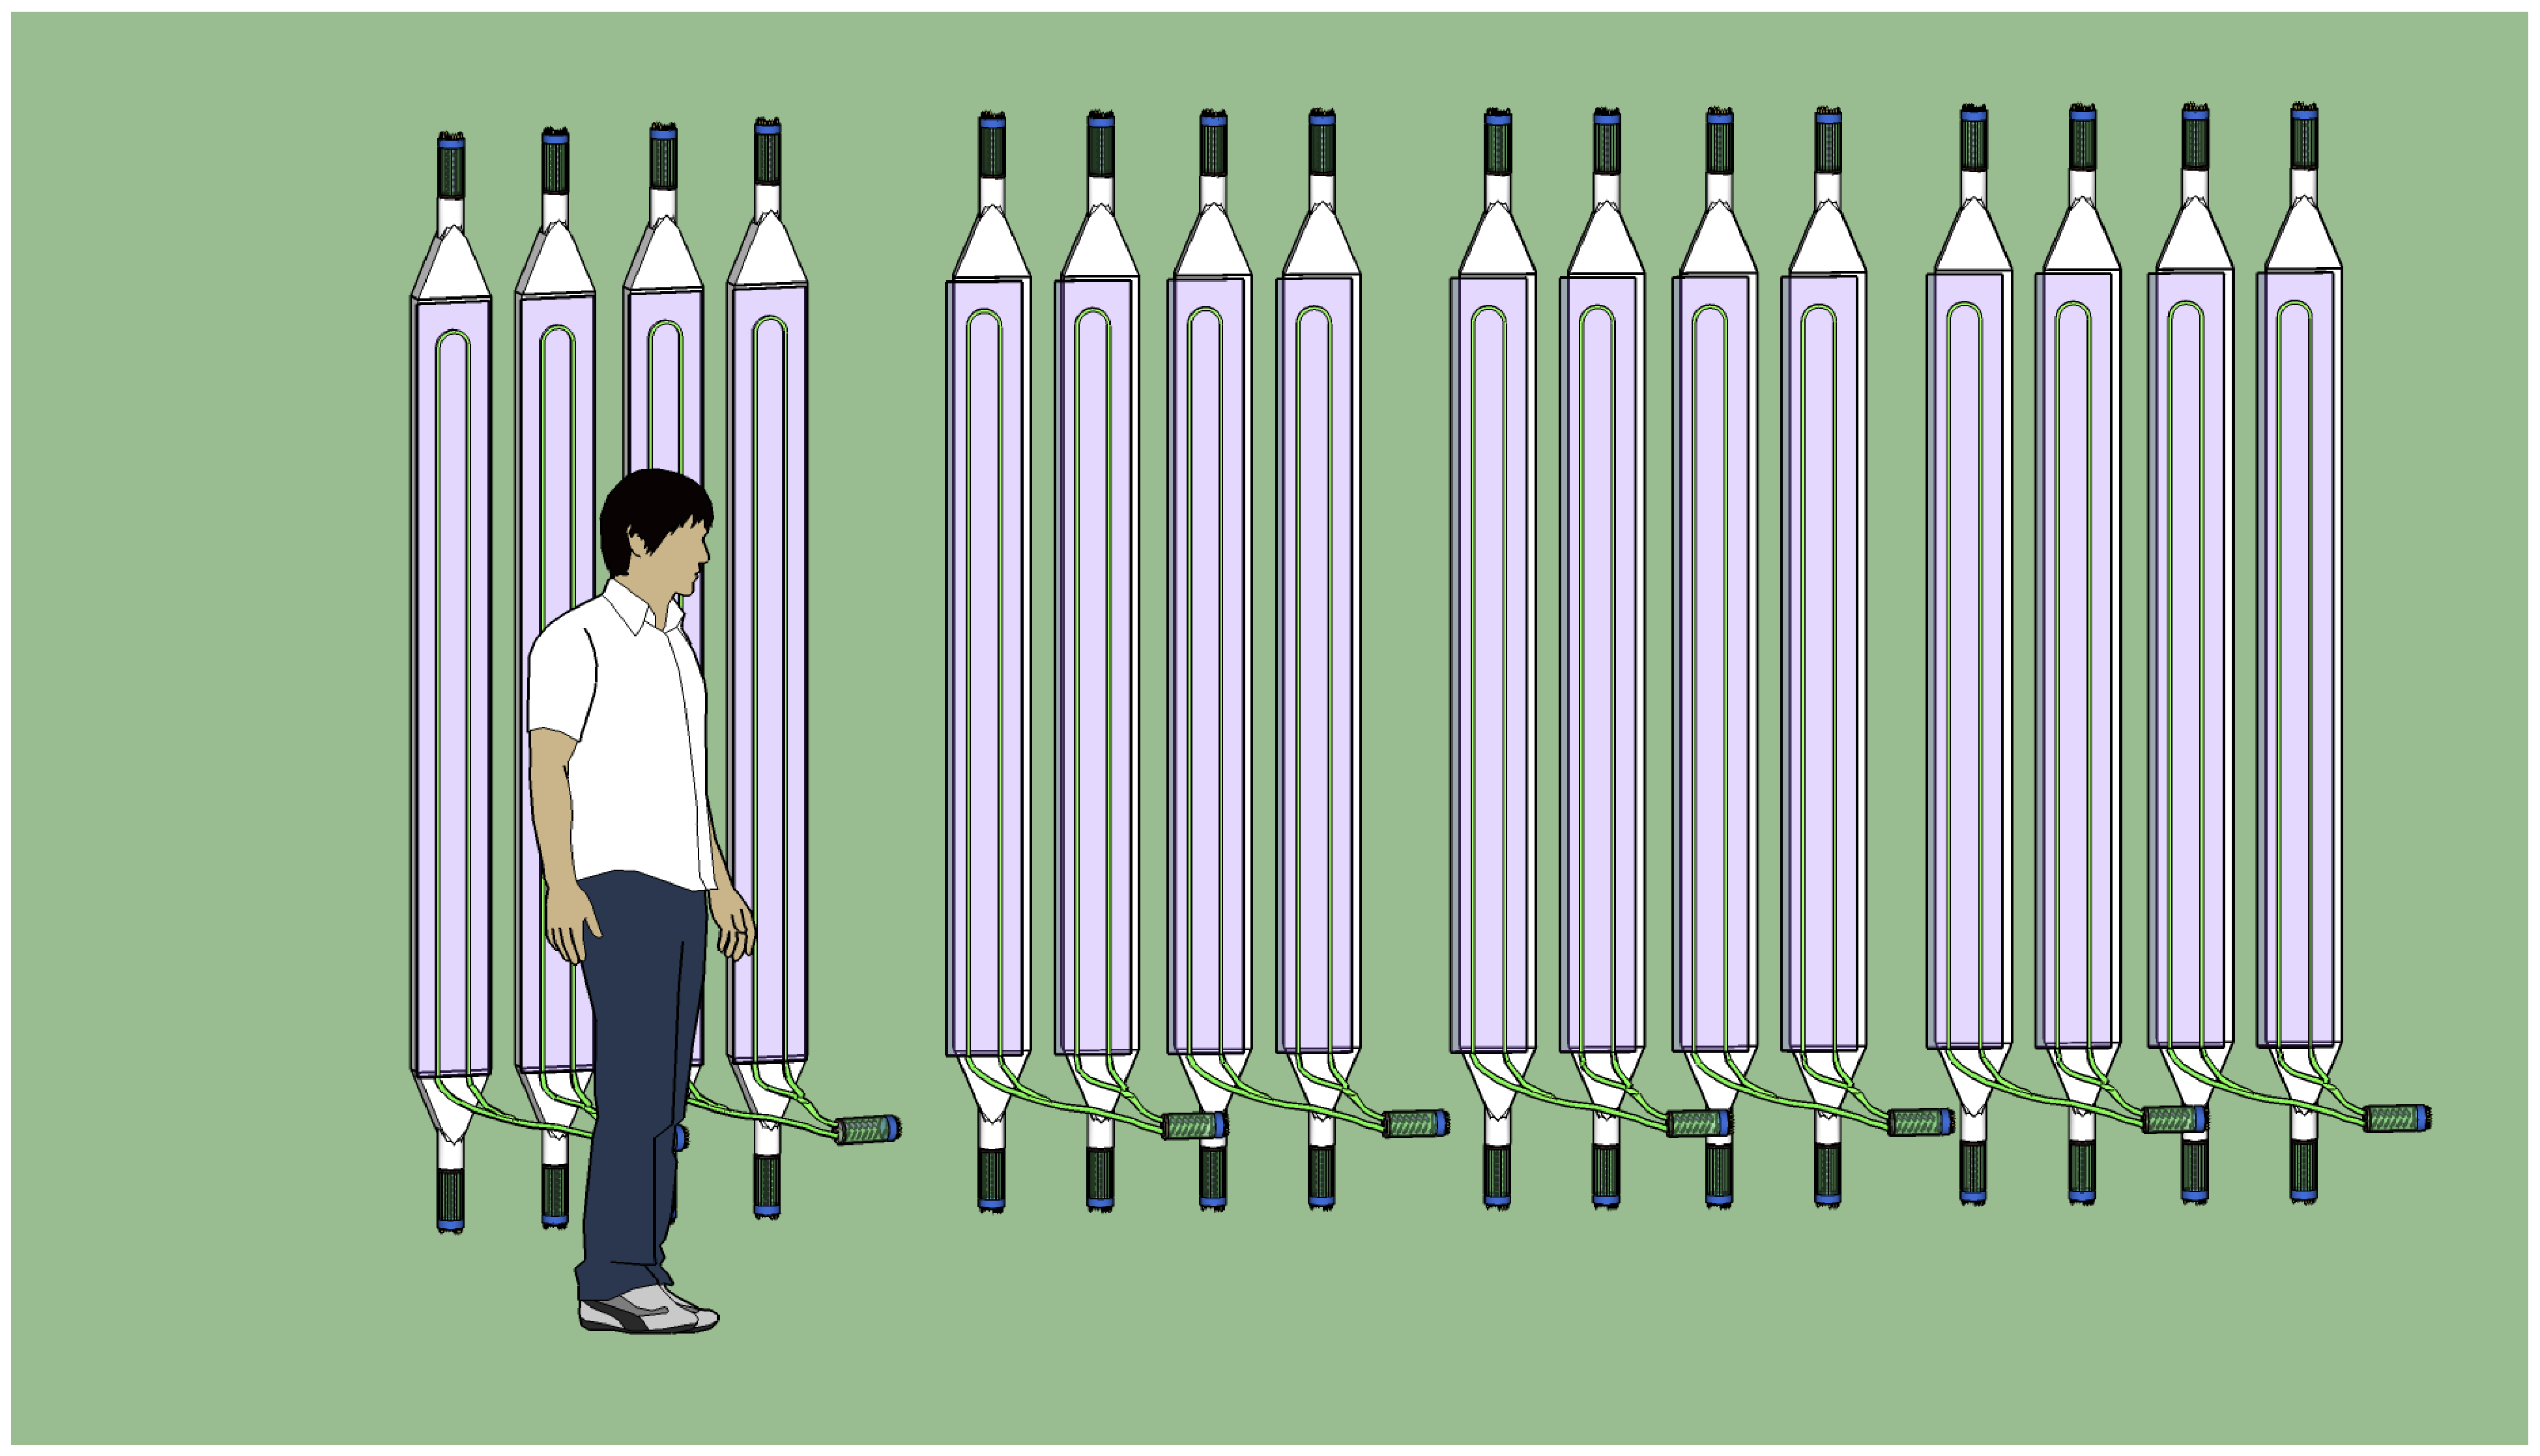
\includegraphics[width=1.0\textwidth]{figures/neutwall_Oct18.eps}
\caption{The final arrangement of the veto paddles on the neutron detector.  The distance between the veto paddles and the bars of the neutron detector have been minimized.  Note also the addition of veto material on the sides of the neutron detector sub-units.}
\label{fig:vetoSetup}
\end{figure}

\begin{figure}[htp]
%\centering
%\includegraphics[width=1.0\textwidth]{figures/finalBackground.eps}
\vspace{3in}
\caption{Room background after rejection by the veto.  Note that the average and the spread are both reduced from that of the initial setup.}
\label{fig:finalBackground}
\end{figure}

\section{Electronics}
\begin{comment}
Originally wanted to use timing information but there weren't enough channels
Bit Register - give example
discuss random rate and estimate how often you'll fire during a real event and also how often one bar will fire with something real, vetoing a real event
LeCroy 4532 - MALU - majority logic unit ``The status of up to 32 inputs can be monitored and recorded by issuing a strobe.  Since the inputs are edge-triggered, the strobe may be a gate of arbitrary duration.  Then any inputs which are on during any portion of the gate are recorded and stored in a pattern register.'' (from the manual).
\end{comment}
As mentioned above in {\sect}~\ref{sec:singleVeto}, tests on single veto paddles were done using a timing spectrum.  Recording time information for the full veto was not practical, and two bit registers were used instead.  A bit register has several inputs, each corresponding to a bit in an integer, and a gate.  When the gate is high, the bit register records the bit pattern built by the voltages on its inputs; its output is the integer corresponding to this bit pattern.  This integer is a unique representation of which bars fired during the time specified by the gate.  If the gate used is the Event signal from the neutron detector, the bit register will record which veto paddles fired during an event of interest.  Two 16-channel LeCroy 4532 bit registers were able to instrument all the veto paddles.  The gate signal was a 200~ns-wide copy of the event trigger.

Recording the integer generated by the bit register instead of the time of the signal relative to the beam bunch is a loss of information.  The maximum time difference between an event in the neutron detector and an event in the veto that will still be recorded in the bit pattern is the width of the gate signal, 200 ns.  This compares unfavorably to the timing spectrum, where even with a leading edge discriminator, the timing peak has a width of less than 5 ns.  The concern is that this loss of precision in timing information will lead to unacceptable vetoing of real events.  

Several sources contribute to non-beam-related background radiation, resulting in a beam-off rate in a neutron detector bar of $\sim$1000~Hz.  While some of these events are due to muons, but they have a rate of 1~Hz/ft$^2$ and are therefore a small part of the beam-off noise rate.  The beam-off rate, then, serves as a suitable rate with which to calculate an upper bound for the rejection of beam-related events.  The probability that a noise event will occur within the window allowed by the bit register and veto a beam-related event is
\begin{equation}
\text{P(A)}\times\text{P(B)} = \text{R}_{\text{n}}\tau_{\text{bit reg.}}\times\text{R}_{\text{beam}}\tau_{\text{beam}},
\end{equation}
where A is a noise event recording in the bit register and B is a beam-related event that has triggered the DAQ.  The probability of a veto scales with the noise rate $\text{R}_{\text{n}}$ and beam-related event rate $\text{R}_{\text{beam}}$ as well as the time window of the bit register $\tau_{\text{bit reg.}}$ and DAQ event $\tau_{\text{beam}}$.  With a noise rate of 1000 Hz, a bit register window of 200 ns, and an event window of 1000 ns, the probability of the a vetoed beam-related event is $2\times10^{-10}\text{R}_{\text{beam}}$.  This fraction of vetoed events is less than 1\% and will not have any statistical significance, even with the timing resolution lost by moving to a bit register.  A schematic of the veto electronics is shown in {\fig}~\ref{fig:vetoElectronics}.  Note that no changes to the DAQ other than the addition of the bit register are required.
\begin{figure}[htp]
\centering
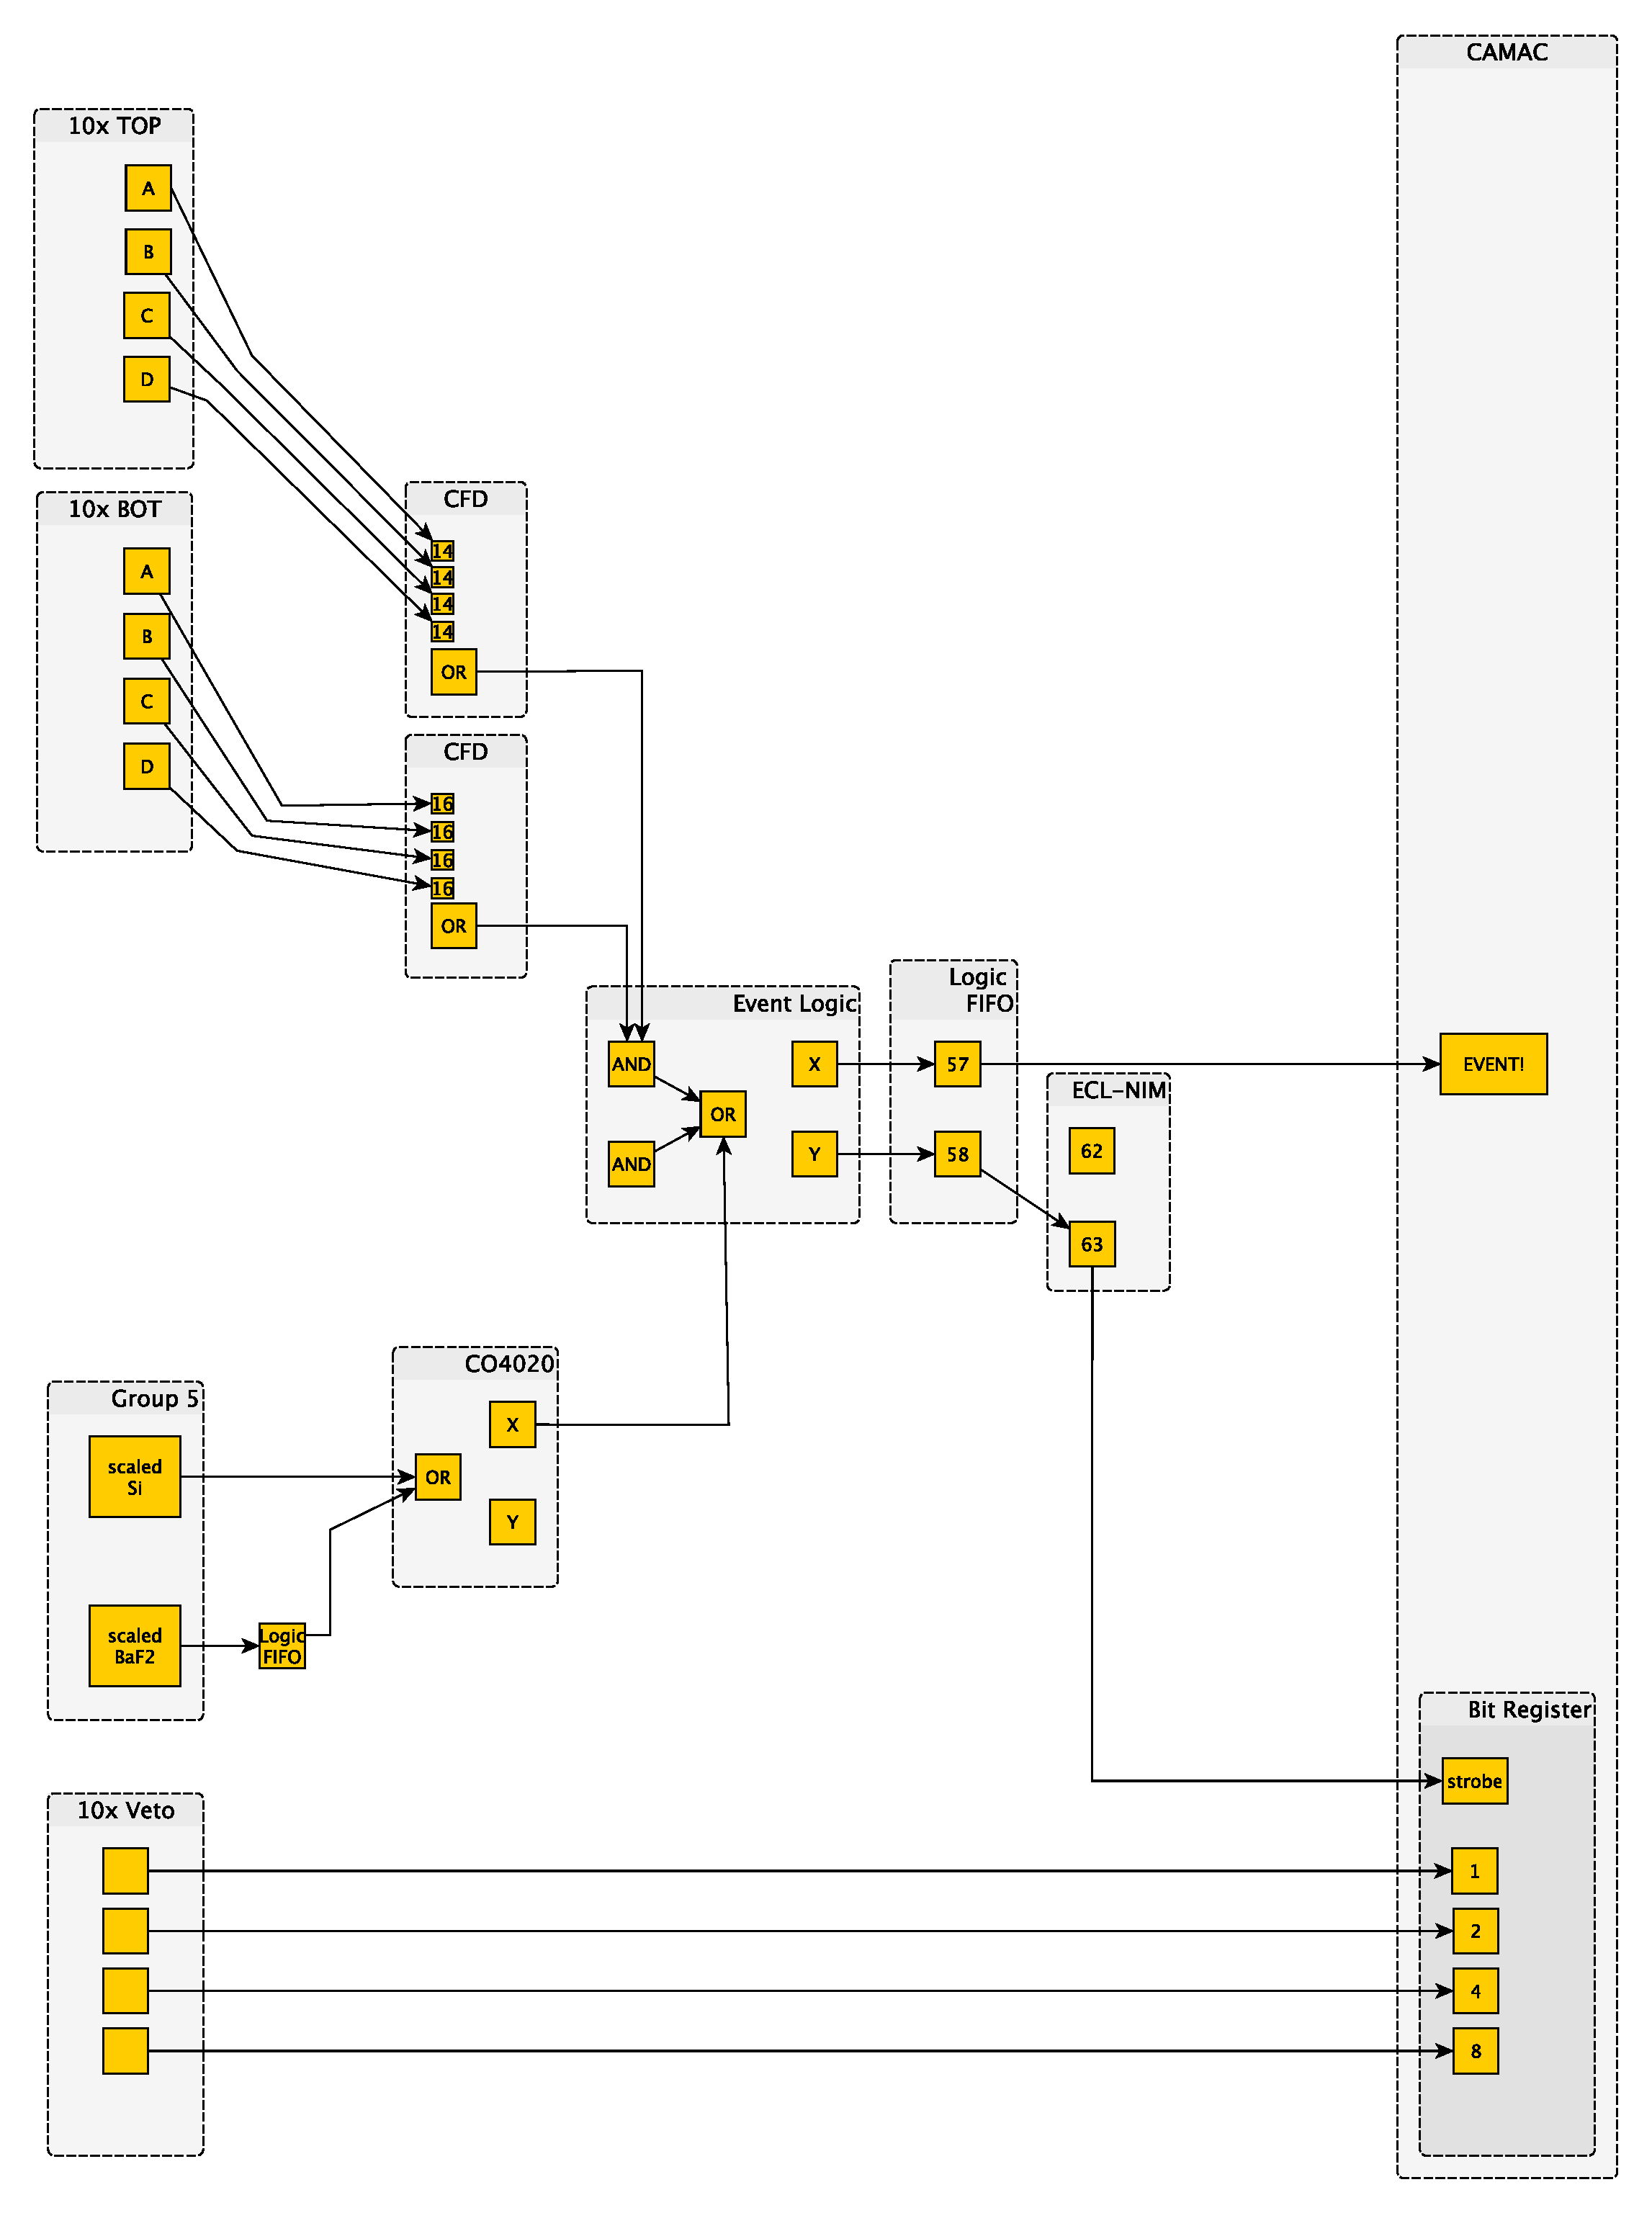
\includegraphics[width=1.0\textwidth]{figures/electronics_veto.eps}
\caption{The integration of the veto electronics with the existing DAQ.  The bit register is used in the data analysis.  Scalers are also added for run-time monitoring.}
\label{fig:vetoElectronics}
\end{figure}
 

\section{Beam Tests}
\begin{comment}
What data should I show?  Old Mg vs. New Mg?  Or New Mg with no veto vs.  New Mg with veto?
show the vetoed spectrum - put a limit on how much real signal is rejected?
\end{comment}
The background rejection of the assembled veto system is approximately 90\% as can be seen in {\fig}~\ref{fig:veto_26Mg}.  The rejection is strongly dependent on energy cuts placed on data; with lower energy cuts, gamma radiation contributes significantly to the background, and the veto is not effective.  90\% rejection is typical of cuts that are above the thorium edge.  Although such a high bound on the energy discards many neutron events, it also rejects more of the background $\gamma$ radiation and maximizes the signal/background ratio.See figure ?? for a description of the rejection as a function of the energy cut. 

\begin{figure}[htp]
\centering
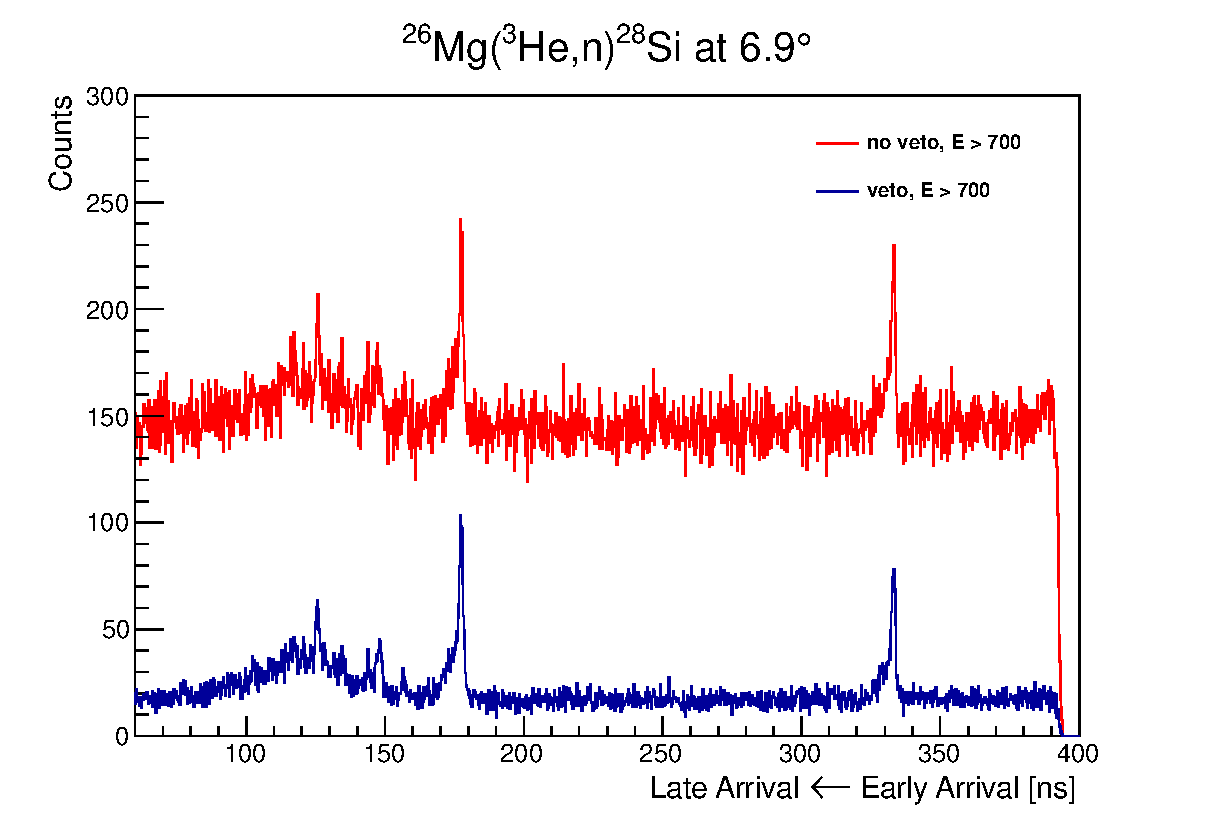
\includegraphics[width=5in]{figures/veto_26Mg.eps}
\caption{\label{fig:vetoData}The effect of the veto on the $^{26}$Mg($^3$He,n) data.}
\label{fig:veto_26Mg}
\end{figure}

The reduced background significantly improves the data we were able to obtain on \MgReaction.  Errors on the ground state transition were reduced from 7\% to 3\%.  Most importantly, the signal strength that we now have 2$\sigma$ sensitivity to when running at a beam current of ?? for one week is ??, down from ??.  This is crucial for investigating the distribution of the \zp state in \GeTargets.

\subsection{Rejected Signal}
\begin{comment}
Two causes for rejected signal
1. the bars are ganged together; could get a signal in one veto bar that does not mean there was a cosmic in its adjacent neutron detector
2. randoms

can place a limit on randoms, reals, and therefore good rejected signal
\end{comment}
While the achieved background rejection is excellent, it is important to consider how often the veto rejects real neutron events.  Such a rejection could occur when a neutron interacts in both the veto and the neutron detector, when the neutron detector sees a real signal and the veto triggers from an uncorrelated event such as a background gamma, or when a neutron interacting in the detector kicks out a proton that triggers the veto.  This last case should occur very rarely; this is the primary reason we chose to mount the veto on the front of the detector.  It is also possible for the veto to absorb a neutron that could otherwise interact in the detector.  In all cases, the vetoing of real events will result in timing peaks that sit on top of the flat, random background of the rejected events.  {\fig}~\ref{fig:rejectionTOF} shows the rejected events for all current \Mg{26} data; no peak is visible.  Given the background, this places a limit on the total rejection of real neutron events at ?? at a 90\% confidence level.  
\begin{figure}[htp]
\centering
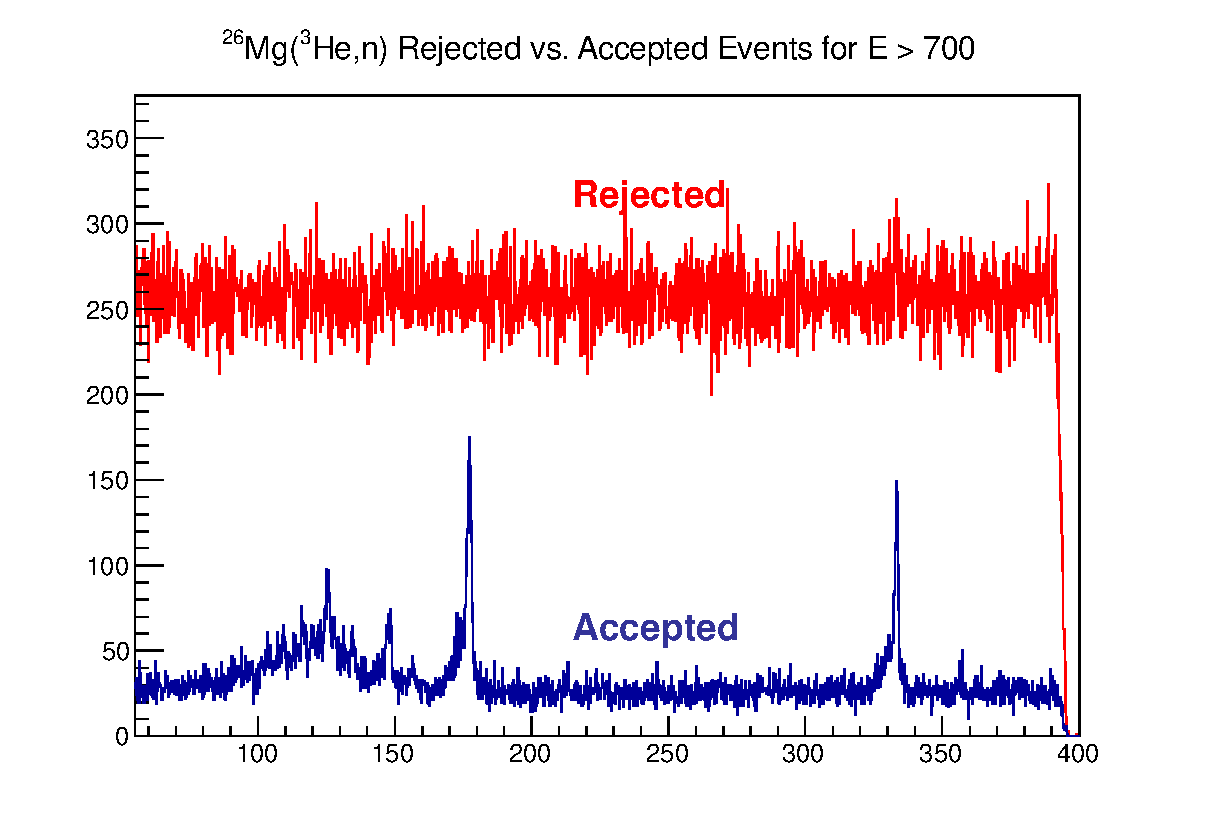
\includegraphics[width=5in]{figures/26Mg_rejection.eps}
\caption{\label{fig:rejection}A plot of the rejected events.  Peaks in the rejected spectrum are from real, vetoed events.  No neutron peak is visible; there is a small peak from rejected gamma events.}
\label{fig:rejectionTOF}
\end{figure}

Testing with \MgReaction demonstrates that the muon veto reduces background by $\sim$90\% and does not veto a significant number of beam-related events.  In addition to verifying the proper functioning of the veto system, this reaction also measures the efficiency of the neutron detector because the cross-section is well known.  These efficiency calculations, as well as the data from the \GeTargets experiments, will be discussed in the next chapter.


% % uncomment the following lines,
% if using chapter-wise bibliography
%
% \bibliographystyle{ndnatbib}
% \bibliography{example}




%
% Chapter 5
%

%
% Modified by Sameer Vijay
% Last Change: Wed Jul 27 2005 13:00 CEST
%
%%%%%%%%%%%%%%%%%%%%%%%%%%%%%%%%%%%%%%%%%%%%%%%%%%%%%%%%%%%%%%%%%%%%%%%%
%
% Sample Notre Dame Thesis/Dissertation
% Using Donald Peterson's ndthesis classfile
%
% Written by Jeff Squyres and Don Peterson
%
% Provided by the Information Technology Committee of
%   the Graduate Student Union
%   http://www.gsu.nd.edu/
%
% Nothing in this document is serious except the format.  :-)
%
% If you have any suggestions, comments, questions, please send e-mail
% to: ndthesis@gsu.nd.edu
%
%%%%%%%%%%%%%%%%%%%%%%%%%%%%%%%%%%%%%%%%%%%%%%%%%%%%%%%%%%%%%%%%%%%%%%%%

%
% Chapter 4
%

\chapter{DATA ANALYSIS}
\label{chap:dataAnalysis}
\begin{comment}
We care about two things:
1. The absolute cross-section of the ground state transition
2. Setting a limit on excited 0+ state cross-sections
\end{comment}
The aim of the analysis of the \reaction data sets is to extract the absolute cross section of the reactions populating the ground states of \SeProducts and also to set a limit on excited \zp-state cross sections.  Each of these analyses is discussed in its own section, but because the absolute cross section is of interest, the detector efficiency and several other properties of the experiment must be accurately determined.  The measured quantities used most frequently in this analysis are the timing relative to the beam bunch and the light signal.  ``Time'' in this chapter always refers to the arithmetic average of a bar's top and bottom time values.  A timing spectrum is shown in {\fig}~\ref{fig:time}.
\begin{figure}[!htbp]
\centering
\subfloat[][]{
   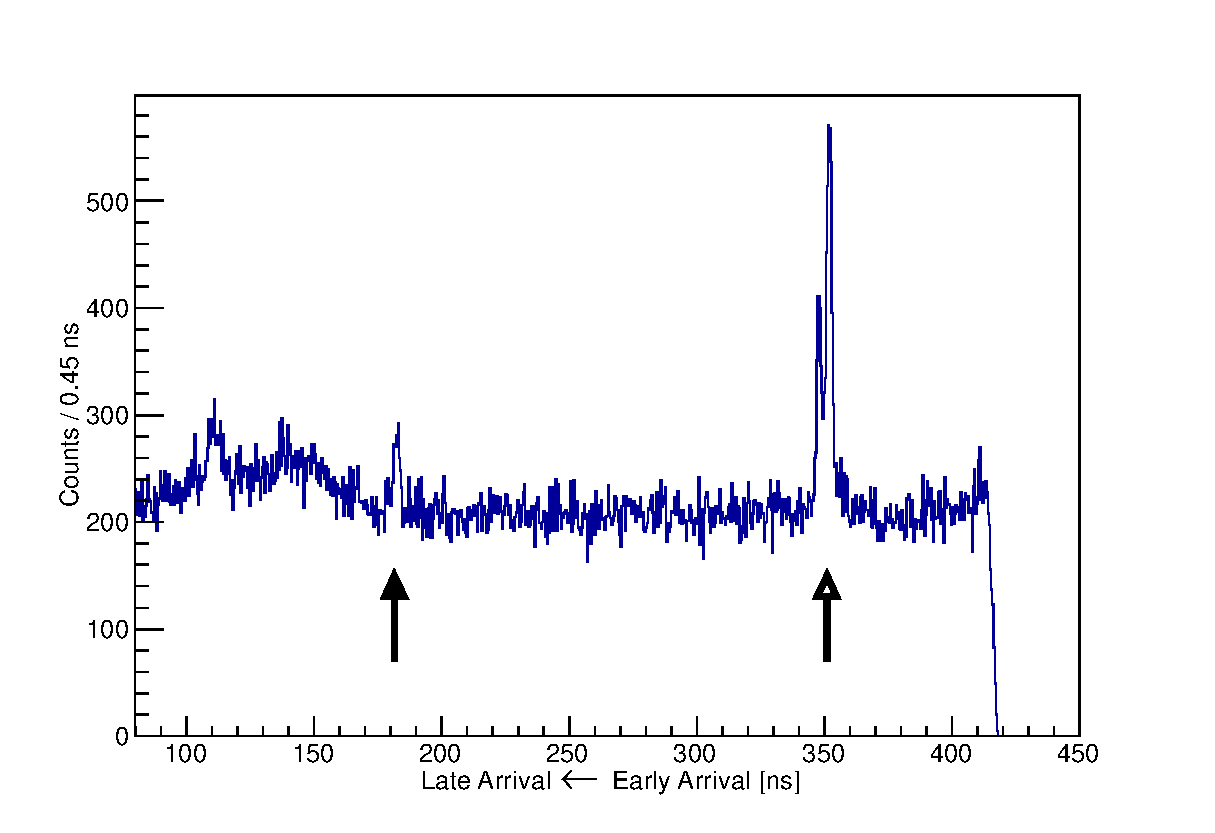
\includegraphics[width=0.5\textwidth]{figures/74Ge_sep_PS_barA.eps}
}
\subfloat[][]{
   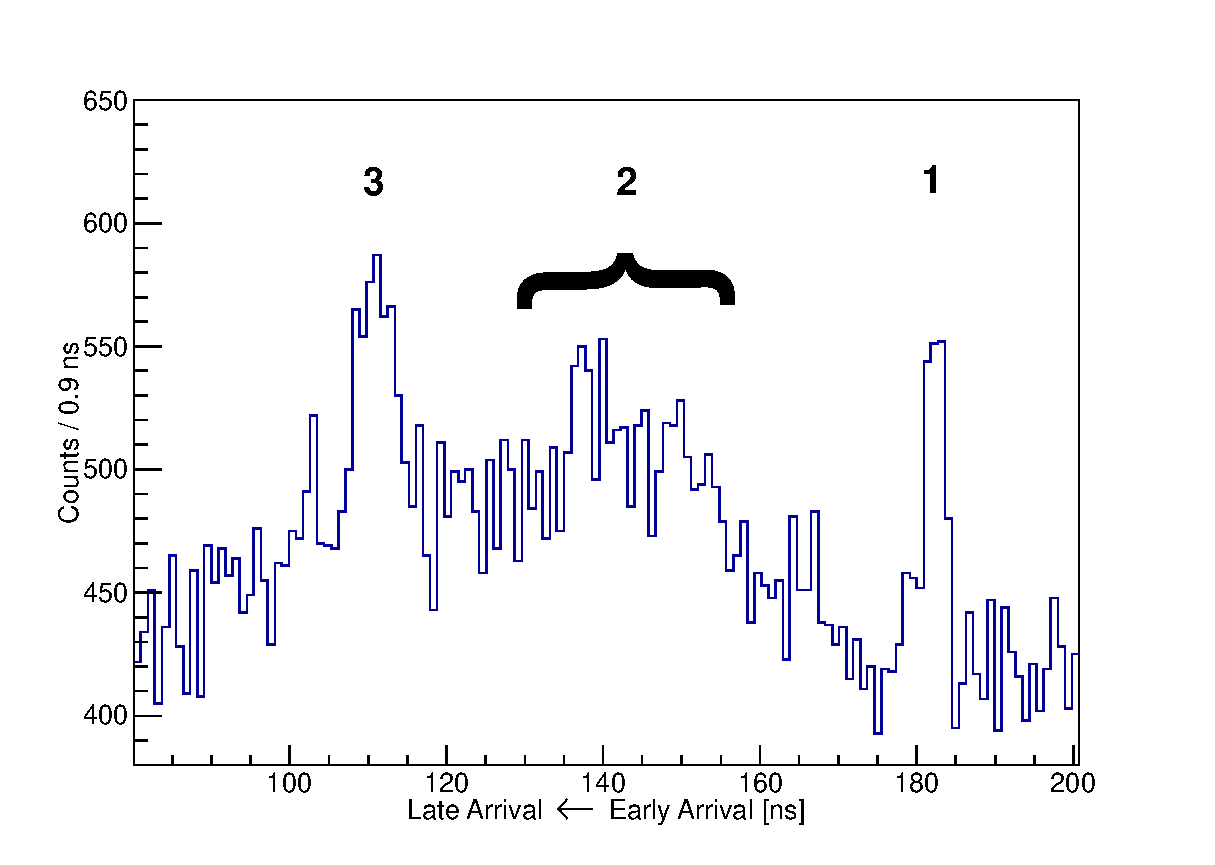
\includegraphics[width=0.5\textwidth]{figures/74Ge_sep_PS_barA_zoom.eps}
}
\caption{(a) A (time of flight) (TOF) spectrum from the forwardmost neutron detector bar (6.1$^{\circ}$) in the case of pulse-selected beam.  The reaction is $^{74}$Ge($^3$He,n)$^{76}$Se.  The ground-state neutron peak is indicated with a solid arrow and the $\gamma$ peak with a hollow arrow.  Note that the $\gamma$ peak is doubly peaked, from beam hitting the target and then the beamstop.  (b) The neutron spectrum.  The ground-state neutron peak is indicated with a ``1'', the neutron continuum with a ``2''.  The other prominent peak, labeled ``3'', is due to oxygen contamination in the target.}
\label{fig:time}
\end{figure}
Another measurement important for analysis is the integrated light output at the top and bottom of a bar.  A geometric average of these, $\sqrt{E_tE_b}$, where $E_t$ and $E_b$ are the integrated light signal of the top and bottom PMT, respectively, is considered a measure of the neutron energy and is referred to as ``energy'' in this chapter.  This quantity is discussed further in {\sect}~\ref{sec:cuts}.   The top and bottom PMT signals, taken separately, are not necessarily a measure of the energy of the event and will be referred to as ``light signals'' when used without averaging. 
% geometric average used twice, rewrite 

% a basic discussion of the data:
% TOF spectrum explained
% energy estimator

\section{Detector Efficiency}
\begin{comment}
deuterium, Mg, cuts
\end{comment}
\label{sec:efficiency}
The number of counts due to neutrons measured by the detector scales linearly with the absolute cross section of \reaction but must be corrected for the fact that not all the neutrons leave a signal in the detector.  The ratio of the detected neutron flux to the total neutron flux is called the efficiency of the detector and must be carefully determined as its error contributes directly to the systematic uncertainty of the extracted absolute cross sections.

The efficiency of a plastic-scintillator-type neutron detector depends not only on the energy of the neutron, but also on the detector's size, shape, energy resolution, and detection threshold.  A Monte-Carlo code developed by Cecil \cite{Cecil_neutEfficiency} calculates the efficiency of plastic scintillator detectors for a wide range of neutron energies and detector thresholds to within 10\%.  The Cecil code was used to calculate efficiencies of the neutron detector for neutrons with energies of 10-28~MeV.  The efficiencies predicted by the Cecil code were verified against d(d,n) and \MgReaction measurements, both of which have well-known cross sections.  Comparing the calculated efficiency to measured efficiency over a range inclusive of the neutron energies produced in \reaction gives confidence that the code accurately models the detector.   The inputs required by the code are the density of the detector, its hydrogen to carbon ratio, the energy threshold applied to the data, and the interval over which the detector averages the light output, i.e., the resolution of the detector.  The plastic properties are reported in {\tab}~\ref{tab:WLS_Kuraray}, and the threshold and resolution of the detector must be determined from the energy spectrum of the selected events from the experiment.  The cuts applied to the data are discussed in {\sect}~\ref{sec:cuts}.  An energy spectrum of the ground-state neutrons of any of the reactions studied can be produced by gating on the ground-state peak in the TOF spectrum.  The energy spectrum for the ground-state neutrons from \MgReaction is shown in {\fig}~\ref{fig:lowEnergyCut}. 
\begin{figure}[!htbp]
\centering
\includegraphics[width=0.8\textwidth]{figures/Lite_28MeV.eps}
\caption{The light curve for 28-MeV neutrons from \MgReaction is obtained by restricting the events to those in the ground-state peak window.  The data points shown in red are from the January dataset.}
\label{fig:lowEnergyCut}
\end{figure}
The width of the high-energy falloff gives the resolution of the detector, and the threshold can be determined by assuming the scale has a zero offset.  That this is a reasonable assumption is confirmed by the accuracy of the calculation.  

The efficiencies calculated using the above method must be checked for absolute accuracy of the prediction as well as accuracy of its predicted dependence on the energy of the detected neutron.  The reaction d(d,n), measured at beam energies near 9~MeV \cite{deuteronCrossSections}, produces ground-state neutrons and is particularly useful because the neutron energy changes drastically as a function of angle, making it a useful check on the energy dependence of the Cecil prediction.  Additionally, empirical fits as described in {\refref}~\cite{deuteronCrossSections} provide excellent estimates of the absolute cross section in this energy region.  The agreement is excellent, as can be seen in {\fig}~\ref{fig:DeuteriumMatch}, which shows the prediction with and without correcting for neutron energy.  This result suggests that the Cecil code accurately adjusts the detector efficiency for neutron energy.  
\begin{figure}[!htbp]
\centering
\includegraphics[width=0.8\textwidth]{figures/deuteriumMatch.eps}
\caption{The prediction for d(d,n) (solid line) matches the data well when the efficiency is corrected for the neutron energy (red points).  The blue points represent the differential cross section where the efficiency is assumed to remain constant despite a changing neutron energy.}
\label{fig:DeuteriumMatch}
\end{figure}

That the Cecil code appears to be successful in calculating the efficiency of the neutron detector for 12-MeV neutrons is encouraging, but neutrons from the ground states of \reaction will be $\sim$26~MeV.  A reaction with measurements of cross sections for neutron energies in this range is \MgReaction.  While this reaction has not been measured at the beam energy of 16~MeV, which would produce a $\sim$28-MeV ground-state neutron, it has been measured at lower and higher energies \cite{MgCrossSection1,Bohne_Mg} as shown in {\fig}~\ref{fig:efficiencyCalib}.  The efficiency measured for the neutrons from this reaction provides a measurement very near the $\sim$26-MeV neutrons produced in \reaction and can be used to verify the absolute efficiency predicted by the Cecil code at neutron energies relevant to \reaction.  {\fig}~\ref{fig:efficiencyCalib} shows the consistency of the measured cross section using that predicted efficiency.  While the agreement between measured cross-sections suggests a systematic error due to efficiency of less than 10\%, the estimated systematic error of the data from \MgReaction is $\sim$20\% \cite{MagensiumCrossSection1,Bohne_Mg} and does not provide a better bound than the error associated with the Cecil code.
\begin{figure}[!htbp]
\centering
\includegraphics[width=0.8\textwidth]{figures/magnesiumMatch.eps}
\caption{Checking consistency of efficiency calculation with \MgReaction.  Black squares shown previous experimentally-measured values of the cross section.  This work (green triangle) is consistent with calculations.  The calculations (red circles) are coupled-channel DWBA calculations following the prescription of \cite{MgCrossSection1}.  The blue lines indicate the estimated systematic error of the calculation.}
% circles - CCBA
% blue lines estimate of systematic error due to CCBA parameters
% squares are existing data
\label{fig:efficiencyCalib}
\end{figure}

\section{Experimental Parameters Related to the Cross Section}
\begin{comment}
current, tgt thickness (RBS), solid angle, dead time
go ahead and discuss errors while you discuss these quantities
\end{comment}

The differential cross section is the number of times a reaction occurred ($N_{reaction}$) normalized by the total number of particles incident on the target ($N_{beam}$), the number density of nuclei in the target ($n_{target}$), and the {efficiency of the detector}~($\epsilon$):
\begin{align}
\frac{d\sigma}{d\Omega} &= \frac{N_{reaction}}{N_{beam} \times n_{target} \times \epsilon}.
\label{eq:cross_section}
\end{align}
The efficiency $\epsilon$ of the detector includes the solid angle $d\Omega$.  Other quantities in the cross section that relate to the experimental setup are the number of particles incident on the target and the number density of nuclei in the target.

The three targets (\GeTargets and \Mg{26}) used in the experiments were provided by John Greene of Argonne National Laboratory (ANL).  The \GeTargets targets were evaporated onto a gold backing, while the \Mg{26} target is self-supporting.  The isotopic abundance and thickness of each target is shown in {\tab}~\ref{tab:targets}.  The target thicknesses were measured with an alpha-thickness gauge when they were made, and again at Hope College using Rutherford back-scattering (RBS).  RBS measurements are useful because they give information about the target composition, which must be assumed when calculating target thickness from alpha-thickness-gauge measurements.  The reported thicknesses were obtained by analyzing the RBS data with SIMNRA \cite{SIMNRA}, an RBS analysis software.  A sample of the fit for each target is shown in {\fig}~\ref{fig:RBS_sample}.  Measurements taken at several different positions on each target showed that variations in target thickness were approximately 1\%.  The predominant features of the RBS spectrum are the plateaus due to the germanium layer and the gold foil.  These plateaus overlap, but the features due to beam scattering from the front and back surface of each layer are clearly visible.  {\fig}~\ref{fig:RBS} and {\fig}~\ref{fig:rawDataRBS} identify these features.  This RBS spectrum also shows evidence of small pinholes in the target; they introduce a low-energy aluminum spectrum that is highlighted in red in {\fig}~\ref{fig:RBS}.  There are also small areas of the target that are bare gold foil, evidenced by the very small plateau at high energies that is highlighted in green.  These features do not alter the estimate of the target thickness, which depends only on the edges of the plateau.  Because the edges of the plateau are well defined, the uncertainty in the number of target atoms is less than a percent.  A cautious estimate of the uncertainty in the cross section due to the target is 2\%.  A fit to the data adjusted for the pinholes is shown in {\fig}~\ref{fig:RBS_sample}. 
\begin{figure}[!htbp]
\centering
\subfloat[][]{
   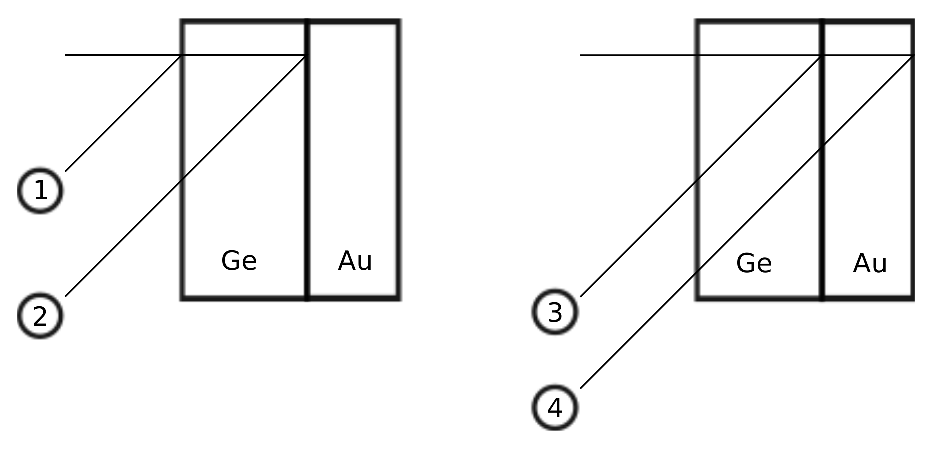
\includegraphics[width=0.5\textwidth]{figures/RBS_possibilities.eps}
   \label{fig:RBS}
}
\subfloat[][]{
   \includegraphics[width=0.5\textwidth]{figures/76ge-4-holes.eps}
   \label{fig:rawDataRBS}
}
\\
\subfloat[][]{
   \includegraphics[width=0.8\textwidth]{figures/76ge-4-adjusted.eps}
   \label{fig:RBS_sample}
}
\caption{\subref{fig:RBS} Beam scattering from the front and back layer determines the high and low energy plateau edges.  The scattering angle is shown as forward to compress the figure but was backward at 168$^\circ$ in the experiment.  \subref{fig:rawDataRBS} RBS data for the \Ge{76} target near the beamspot.  The features used to determine the thicknesses of the gold and germanium layers are marked.  \subref{fig:RBS_sample} The RBS spectrum, adjusted by subtracting the background due to pinholes, and its fit.  Fitting the RBS spectrum with and without adjusting for pinholes did not result in any significant differences to the predicted target composition or thickness.}
% move this to text, highlight features in plot
\end{figure}
\begin{table}[htp]
\centering
\begin{tabular}{lllll}
 & \multicolumn{2}{c}{$\alpha$-gauge ($\mu$g/cm$^2$)} & \multicolumn{2}{c}{RBS ($\mu$g/cm$^2$)} \\
\cline{2-3}\cline{4-5}
$^{74}$Ge (98.9\%) & Au$_{\text{nat}}$ & 1011 & Au$_{\text{nat}}$ & 1001 \\
          & $^{74}$Ge & 1057 & $^{74}$Ge & 1016 \\
          &           &      & O$_{\text{nat}}$ & 9 \\[0.35cm]

$^{76}$Ge (92.82\%) & Au$_{\text{nat}}$ & 1069 & Au$_{\text{nat}}$ & 1014 \\
          & $^{76}$Ge & 838 & $^{74}$Ge & 775 \\
          &           &      & O$_{\text{nat}}$ & 4 \\[0.35cm]

$^{26}$Mg ($>$99.55\%) & $^{26}$Mg & 791 & $^{26}$Mg & 685 \\
          &           &      & C$_{\text{nat}}$ & 10 \\
          &           &      & N$_{\text{nat}}$ & 43 \\
          &           &      & O$_{\text{nat}}$ & 52 \\
\end{tabular}
\caption{Target composition and thickness.  The isotopic abundance of the target is listed in parenthesis.  The $\alpha$-gauge measurements were performed at ANL and the RBS measurements at Hope College.}
\label{tab:targets}
\end{table}

To determine the absolute cross section, it is also necessary to know the total number of \He{3} ions incident on the target for each dataset.  One monitor of the beam current is the charge collected by the Faraday cup.  A BaF$_2$ crystal outside the target chamber and a silicon detector inside the target chamber detect $\gamma$ radiation from beam incident on the target and scattered \He{3} beam, respectively.  Both these detectors monitor the product of the target thickness and the beam current.  Data from the silicon detector show that the ratio of \GeTargets to gold does not change throughout the run, demonstrating that the targets are stable throughout the run.  Additionally, the back-scattered peak in the silicon spectrum scaled with the live charge, which is the charge scalar vetoed by the DAQ busy as discussed in {\sect}~\ref{sec:electronics}.  The live charge can therefore be used to scale beam current between runs, making it possible to express \reaction cross sections in terms of the known \MgReaction cross section.

\section{Data Sets}
Two sets of \reaction data are available.  The first was taken in September 2011.  A subset of this data was taken with no pulse selection due to hardware failure.  A second run in January 2012 provided additional data, all taken with pulse selection.  During the January run, data were taken with the \GeTargets as well as \Mg{26} targets to provide an accurate normalization.  The data sets are summarized in {\tab}~\ref{tab:dataSets}.  While the non-pulse-selected data was useful in constraining parts of the pulse-selected background (see {\sect}~\ref{}), it was not possible to estimate the background well enough to obtain useful cross-section data from these runs.  Thus, the non-pulse-selected data appear in this chapter only as a constraint on a fit to the pulse-selected data.
\begin{table}[htp]
\centering
\begin{tabular}{llll}
            & & Live Time (s) & Live Charge ($\mu$C)\\
\hline
January     & PS \Mg{26} & 46460 & 1044 \\
	    & PS \Ge{76} & 78140 & 2919 \\
	    & PS \Ge{74} & 163800 & 5313 \\ \\

September   & PS \Ge{76} & 126200 & 2873 \\
	    & PS \Ge{74} & 116700 & 2619 \\
	    & NPS \Ge{76} & 273700 & 15320 \\
	    & NPS \Ge{74} & 113200 & 10010 \\
\end{tabular}
\caption{Data sets used in the analysis were obtained in two separate runs.  Both pulse-selected (PS) and non-pulse-selected (NPS) data were taken during the September run.}
\label{tab:dataSets}
\end{table}

\section{Cuts}
\label{sec:cuts}
Four sets of cuts were applied to the data to generate a final data set.  The first cut verifies that the recorded event represents a real event rather than noise.  The next cut discards events with too-low light signals, reducing the background due to $\gamma$ radiation.  Two final cuts reduce the muon background; one cut uses the veto, and the other eliminates events with light signals too large to be due to neutrons.

A true event should have energy above the noise level recorded in both top and bottom PMT's.  Additionally, the time signals from the top and bottom PMT's should be correlated.  A typical scatter plot of timing from the top and bottom PMT are shown in {\fig}~\ref{fig:realEvent}.  Requiring correlated top and bottom timing signals is a cut that is applied to all bars in all final data sets.  The other requirement for a valid event is that the light signal be above the noise threshold.  An example of a light spectrum for a single bar is shown with the noise threshold already applied {\fig}~\ref{fig:realEvent}.
\begin{figure}[!htbp]
\centering
\subfloat[][]{
  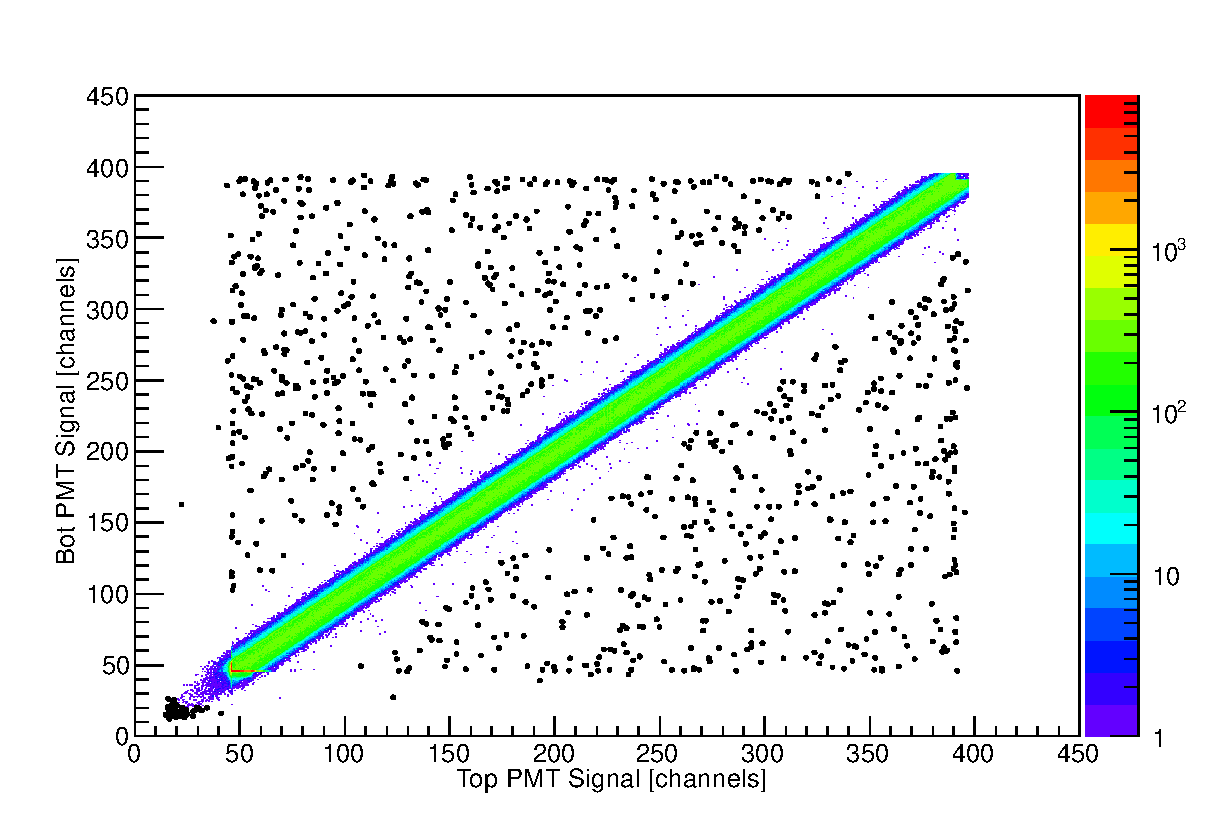
\includegraphics[width=0.8\textwidth]{figures/realTiming.eps}
}\\
\subfloat[][]{
  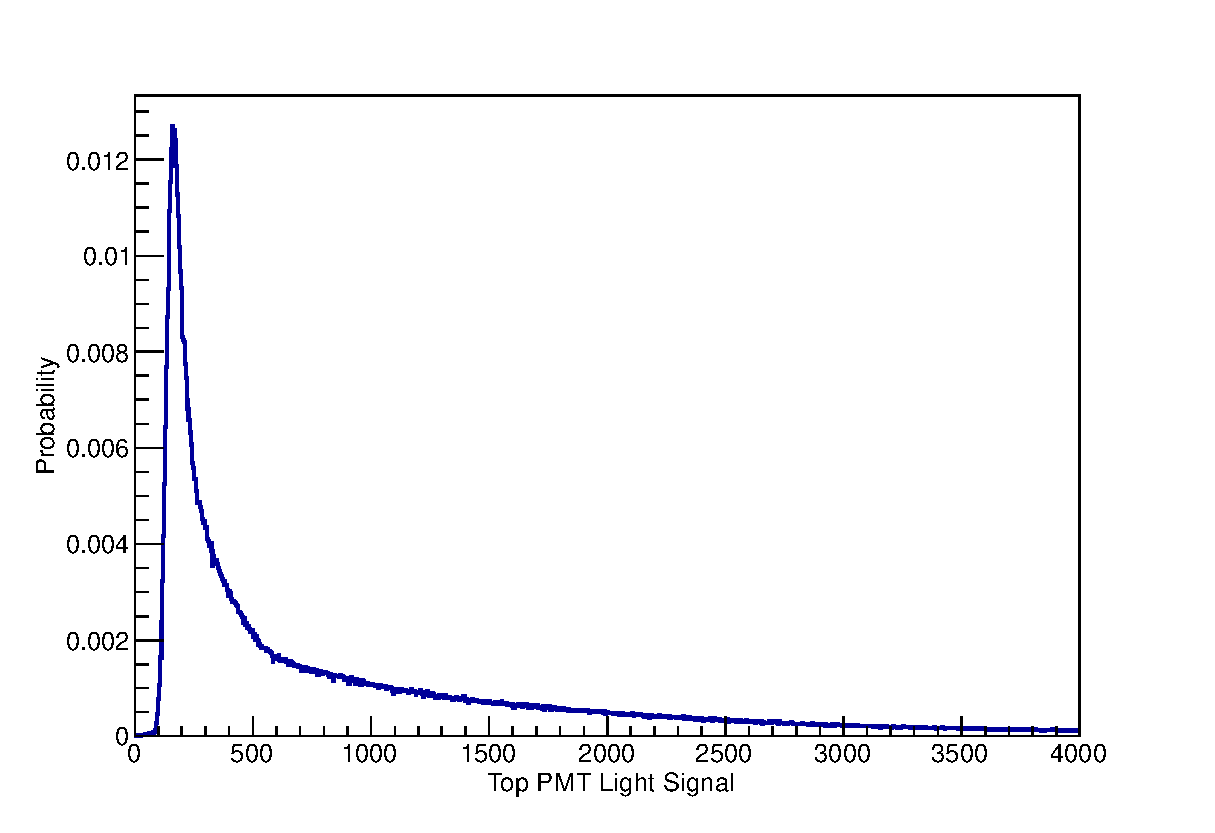
\includegraphics[width=0.8\textwidth]{figures/lightThreshold.eps}
}
\caption{(a) For a real event, the timing signal from a bar's top and bottom PMT will be similar.  Times differing by more than 100 ns are rejected.  Events with correlated timing are shown in color and are inside the thick gray lines.  The larger, black dots indicate events whose timing is not considered correlated.  (b) A low noise threshold placed on the PMT signal discards spurious events.}
\label{fig:realEvent}
\end{figure}

% discussion of muon rejection begins here
Both the veto paddles and the bars of the neutron detector serve as a veto.  Veto paddle information is recorded as either ``true'' or ``false'' - true if a veto paddle fired during the event, false if it did not.  The bars of the neutron detector, in contrast, have more detailed information - time and light output.  While accidental coincidences are rare, this additional information is used when a neutron bar is used as veto material.  For one bar of the neutron detector to veto another, both must have a valid signal and their average time must be similar.

A first approximation to determining whether or not an event is the result of a muon interaction is to require all but one bar in the neutron detector, as well as the entire veto, to be silent.  However, this would veto events that are spatially disconnected and could not possibly be due to a single muon.  To eliminate these unnecessary vetoes, we look at events that register signals in detectors with close spatial proximity, a ``veto group''.  One way to determine the appropriateness of increasing the size of a veto group is by looking at the energy spectrum of vetoed events.  Adding detectors to a veto group that primarily eliminates muons results in an energy spectrum that has roughly equal numbers of high and low energy events, as shown in {\fig}~\ref{fig:muonVetoSpectrum}.  Material that does not veto primarily muon events will yield an energy spectrum that appears much more like the room background spectrum, heavily weighted towards lower energy events, as in {\fig}~\ref{fig:notMuonVetoSpectrum}.  These figures indicate that an appropriate group of material to use in the veto of a detector bar is the immediate, surrounding material.  Several samples of veto groups are shown in {\fig}~\ref{fig:vetoGroups}.  A separate cut to reject muons discards events that deposit energy above the maximum neutron energy deposition.    
\begin{figure}[!htbp]
\centering
\subfloat[][Energy spectrum of a neutron detector bar.  Entries in this histogram are from events having at least one correlated signal in the neutron detector and are likely to be muons.  Notice the high-energy-deposition peak at $\sim$ channel~3000 and its considerable height relative to the low-energy $\gamma$ background.  This low-energy background is dominant in non-muon events as in {\fig}~\subref{fig:notMuonVetoSpectrum}.]{
   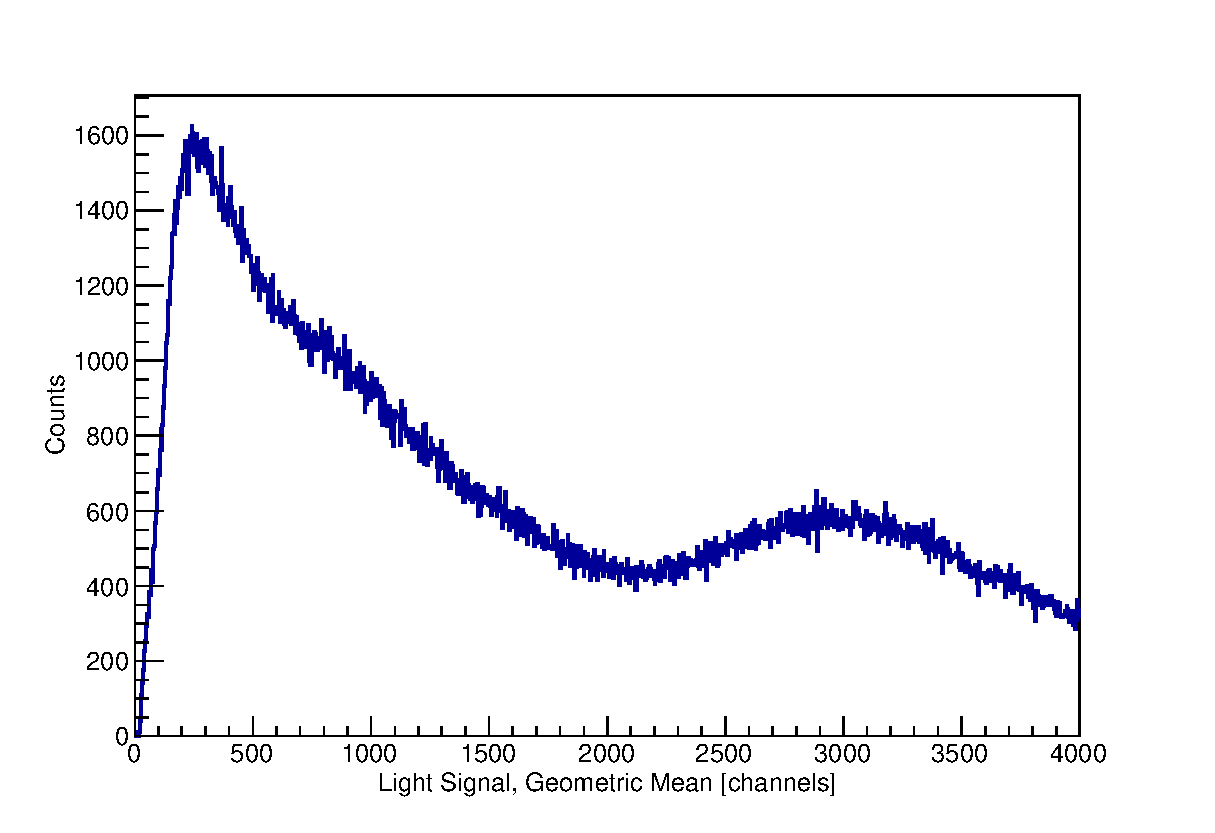
\includegraphics[width=0.45\textwidth]{figures/atLeastOneCorrelatedBar.eps}
   \label{fig:muonVetoSpectrum}
}
\hspace{8pt}
\subfloat[][Neutron detector bar energy spectrum.  These events have no correlation to other signals in the neutron detector and are unlikely to be due to muons.  While some high-energy depositions are visible, the spectrum is clearly dominated by the low-energy peak due to $\gamma$ radiation.]{
   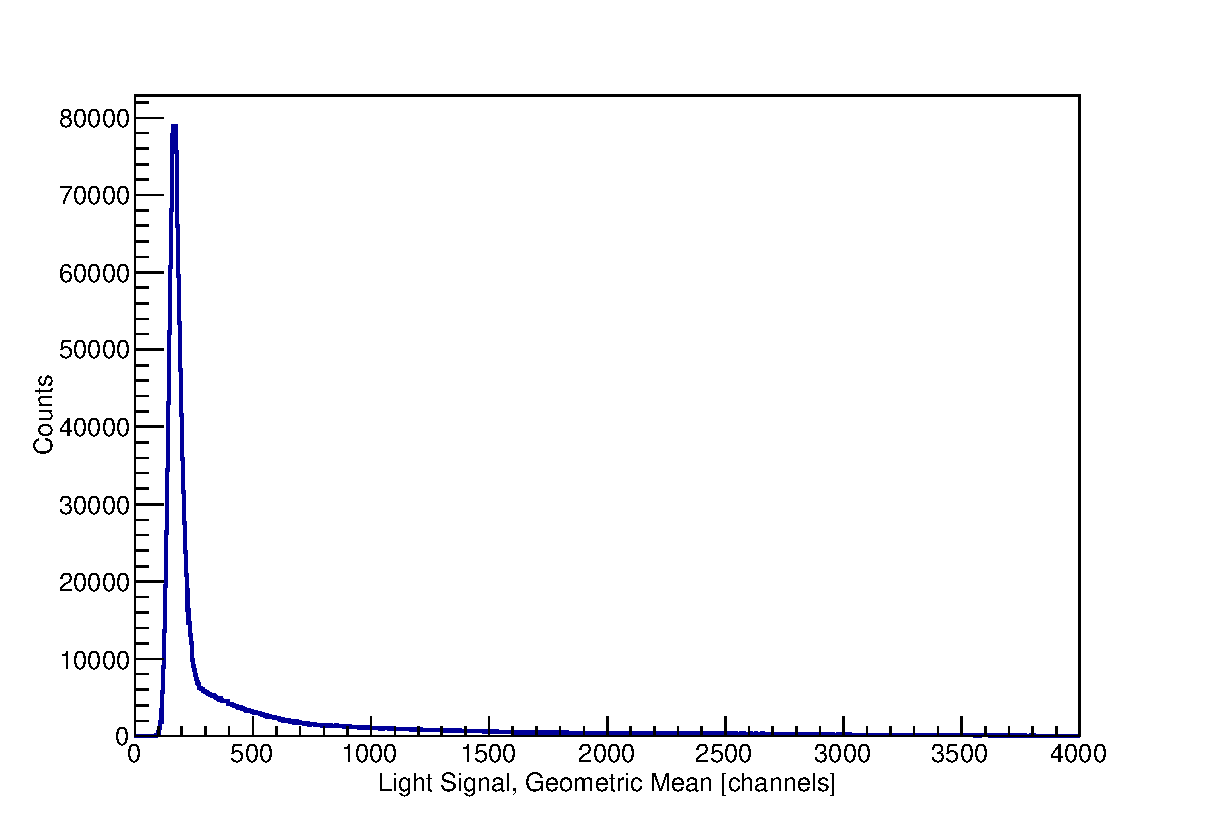
\includegraphics[width=0.45\textwidth]{figures/singleBar_noVeto.eps}
   \label{fig:notMuonVetoSpectrum}
} \\
\subfloat[][Sample groups of detectors chosen to veto bars in the neutron detector.  If the events in a neutron detector bar vetoed by a detector have an energy spectrum dominated by the low-energy $\gamma$ radiation, that detector is not used as part of the veto for that particular bar.]{
   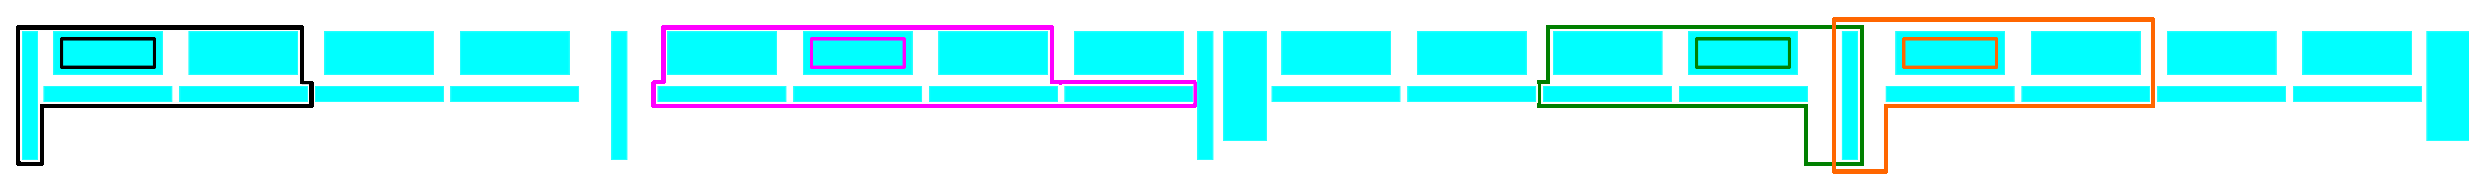
\includegraphics[width=1.0\textwidth]{figures/vetoGroups.eps}
   \label{fig:vetoGroups}
}
\caption{}
\label{fig:determineVetoGroups}
\end{figure}

% discussion of the low energy cut begins here
The final cut on the data sets is a lower-energy cut to reduce the random background due to $\gamma$ radiation.  Placing a low-energy cut on the data is difficult because finding an estimator for the energy is not straightforward.  It is appealing to argue that light loss due to attenuation must be exponential, and that an accurate estimator of the total deposited energy is the geometric mean of the top and bottom PMT signals:
\begin{equation}
\sqrt{Ae^{-\alpha x}\times Ae^{-\alpha (L-x)}} = \sqrt{A^2e^{-\alpha L}} = Ae^{-\alpha L/2},
\end{equation}
where $\alpha$ is a factor determined by the attenuation in the bar and $L$ is its length.  If this model of the signal attenuation is correct, the geometric mean should be position-independent.  This is not the case, as can be seen in {\fig}~\ref{fig:product_positionDependence}.  Furthermore, the position dependence is not often uniform even between the top and bottom PMT on a single bar, making it difficult to construct an average value.  It is necessary to define a low-signal cut that is uniform for all the bars of the detector because the efficiency is sensitive to the low-energy threshold.  It is important to set a uniform threshold on the bars of the neutron detector to avoid introducing significant systematic error into the final cross section.
\begin{figure}[!htbp]
\centering
\includegraphics[width=0.8\textwidth]{figures/positionVSenergy.eps}
\caption{Position dependence of the geometric mean of the light signal of rejected events.  The band of events with light signals between $\sim$1000-1500~channels in particular demonstrates that the signal increases as it approaches the extremes of the neutron detector bar.  The events shown here are those that triggered the veto and are likely muons.}
\label{fig:product_positionDependence}
\end{figure}

Defining a position-dependent light signal cut on each PMT separately would be an ideal solution to these problems if the position dependence for a given energy were known.  While such a characterization of the PMT's for an arbitrary energy is not known, the muon events recorded by the detector do give the light signal as a function of position for one energy.  Due to the detector geometry, it is expected that the average path of the muons will be peaked at slightly more than 5~cm.  Simulations using the detector bar geometry and an angular distribution of $\cos^{2.4}{\theta}$ \cite{cosmicsZenithDependence} (where $\theta$ is the zenith angle) confirm a well-defined peak in the muon path length. This most-likely path length manifests as a peak in the energy spectrum that depends only on the thickness of the bars and on the most likely angle of incident muons because they are MIP's.  Note that both the bar thickness and the most likely angle of a muon path are the same for every bar in the neutron wall.  A simulated energy spectrum is shown next to a real energy spectrum in {\fig}~\ref{fig:muonSpectrum}. 
\begin{figure}[!htbp]
\centering
\subfloat[][]{
   \includegraphics[width=0.5\textwidth]{figures/cosDist_distances.eps}
}
\subfloat[][]{
   \includegraphics[width=0.5\textwidth]{figures/BarA_cosmics_centerSlice.eps}
}
\caption{(a) A simulation of path length of muons interacting in a detector with dimensions identical to those of the neutron detector bars.  Note the distinct peak. (b) Light signal of muon events near the center of the bar.  The peak in this distribution is believed to be the peak seen in the simulated spectrum.}
\label{fig:muonSpectrum}
\end{figure}
The peak of the light spectrum is assumed to represent the same energy and therefore to function as a calibration of the position dependence of the light signal due to the most likely muon energy deposition.  Fits to the location of the energy peak as a function of position are shown in {\fig}~\ref{fig:fits_pkVSpos}.
\begin{figure}[!htbp]
\centering
\subfloat[][The position dependence of the light signal from a single PMT.]{
   \includegraphics[width=0.8\textwidth]{figures/PMT_positionResponse.eps}
} \\
\subfloat[][The two-dimensional histogram shown in (a) is projected into a series of one-dimensional histograms.  The peaks of these histograms are determined by fitting with a Landau function.]{
   \includegraphics[width=0.45\textwidth]{figures/position_sliceGraphs.eps}
}
\hspace{8pt}
\subfloat[][A plot describing the curve which, when scaled, is used as the low-energy cut.  The points are determined from the histograms shown in (b).  Points at the extremes that do not follow the trend are used to determine the position cut.]{
   \includegraphics[width=0.45\textwidth]{figures/EnergyCutExample.eps}
}
\caption{}
\label{fig:fits_pkVSpos}
\end{figure}
Using this ``constant-energy curve'' directly as a lower-energy cut is too high an energy cut as can be seen in {\fig}~\ref{fig:highEnergyCut}.  Instead, a scaling factor is applied to these curves that maximizes the signal to noise ratio; the scaled curves serve as appropriate energy cuts.  While high cuts discard more background, they also discard more neutrons of interest, which can deposit a small amount of energy in the detector.  The minimum fractional error is achieved with a scaling factor that results in a reduction of the background by a factor of $\sim$1.4 (with all other cuts applied).  This is the case for every bar in the neutron detector; the fractional error as a function of the energy cut for the forwardmost bar is shown in {\fig}~\ref{fig:signalToNoise}.  Scaling ratios are determined by comparing the background to that of the initial cut to obtain uniform scaling from bar to bar.  
\begin{figure}[!htbp]
\centering
\subfloat[][The ratio of the signal to its statistical error as a function of the energy cut.  The energy cut is parametrized as the background reduction to allow uniform scaling between bars.]{
   \includegraphics[width=0.45\textwidth]{figures/signalToNoiseCurveA.eps}
   \label{fig:signalToNoise}
}
\hspace{8pt}
\subfloat[][Without applying a scaling factor to the cut determined as in {\fig}~\ref{fig:fits_pkVSpos}, the neutron signals are nearly lost.  Scaling the cut by $\sim$0.5 results in a reasonable signal to noise ratio.]{
   \includegraphics[width=0.45\textwidth]{figures/needLowerCut.eps}
   \label{fig:highEnergyCut}
}
\caption{}
\label{fig:scalingFactorEffect}
\end{figure}
An additional concern is that simply scaling the energy cut may not provide an accurate position dependence.  No distinct feature exists at lower energies, making this difficult to check directly.  However, the position distribution of rejected events with these scaled energy cuts is flat as seen in {\fig}~\ref{fig:flatPositionSpectrum}, suggesting that the position dependence at the most-likely deposited energy for muons is a reasonable approximation for lower-energy events.
\begin{figure}[!htbp]
\centering
\includegraphics[width=0.8\textwidth]{figures/PositionSpectrum2.eps}
\caption{A histogram of event position with a lower-energy cut based on position.  The data used is the \MgReaction data from January.  The difference between the position spectra of the region around the ground state neutron peak (green) and a background region with the same number of bins (blue) is shown in black.  That this resulting position spectrum is flat indicates that the position dependence of the cut is appropriate.}
% rebin
% make sure spectra are clearly visible
\label{fig:flatPositionSpectrum}
\end{figure}

The error associated with the lower-energy cut is non-zero due to the finite energy resolution of the detector.  An estimate of the error on the extracted signal is
\begin{equation}
\sigma_S^2 = \left( \frac{dS}{dE} \right)^2 \sigma_E^2, 
\end{equation}
where $E$ is a variable denoting the low-energy cut.  The uncertainty $\sigma_E$ can be calculated from the resolution of the detector, which is determined by fitting the efficiency calculations to the measured light curve as shown in {\fig}~\ref{fig:lowEnergyCut}.  The change in signal with respect to the energy cut is determined by numerically estimating the derivative in the region of the chosen energy cut.  For this energy cut, which is approximately a third of the maximum deposited neutron energy, the error due to the energy cut is $\sim$8\%.


\section{Ground State Cross-Section}
\begin{comment}
two data sets
- pulse selection
- no pulse selection

background
- gamma peaks - do not overlap with neutron peak
- other neutron peaks - ??
- randoms - background in both data sets
- continuum - more important in non-pulse-selected data

extracting counts 
- pulse selection
- no pulse selection
\end{comment}

To extract the counts due to the ground-state neutrons one can sum the counts in the region of the peak and subtract the estimated background:

\begin{equation}
\text{S = P - B},
\label{eq:counts}
\end{equation}
where S is the extracted number of signal counts, P is the number of counts in the signal region, and B is the number of estimated background counts.  The error associated with $S$ is
\begin{equation}
\sqrt{\sigma_{P}^2 + \sigma_{B}^2}
\label{eq:errDef}
\end{equation}
where both $P$ and $B$ can be understood as a random variable with error $\sqrt{P}$ and $\sqrt{B}$, respectively.

The primary challenge is finding an accurate way to estimate the background that reduces the error of the extracted counts.  As can be seen in {\fig}~\ref{fig:PSvsNPS}, the background of the pulse-selected data is much simpler than that of the non-pulse-selected data.  Without pulse selection, the neutron peak is superimposed on background from previous neutron bunches, making the extracted signal extremely sensitive to poorly-constrained fit parameters.  Only signal estimates from the pulse-selected data are used for the data sets discussed in this thesis.
\begin{figure}[!htbp]
\centering
\subfloat[][]{
   \includegraphics[width=0.5\textwidth]{figures/74Ge_sep_PS_barA.eps}
}
\subfloat[][]{
   \includegraphics[width=0.5\textwidth]{figures/74Ge_sep_NPS_barA.eps}
}
\caption{(a) The TOF spectrum of the forwardmost neutron detector bar (6.1$^{\circ}$) in the case of pulse-selected beam.  The data is from the September run.  The ground-state neutron peak is indicated with a solid arrow and the $\gamma$ peak with a hollow arrow. (b) The timing spectrum of the  non-pulse-selected beam, also from the September run.}
\label{fig:PSvsNPS}
\end{figure}

\subsection{Pulse-Selected Data}
\label{sec:PS_data}
In the case of the pulse-selected data, the background in the region of the ground-state peak consists of flat, random background and the high-energy tail of the neutron continuum.  The $\gamma$-ray peaks are far away from the neutron peak and have no effect.  The random background is well-constrained in the region between the ground-state neutron peak and gamma peak.  The neutron continuum is due to multiple direct reactions and can only contribute to the background of the ground state neutron peak due to detector resolution.  Limits on the contribution of the continuum will be discussed later.  For now, we focus on the simplest contribution to the background, the flat distribution due to random radiation.

In the case of the pulse-selected data, estimating the background is done by fitting the flat background.  In general, the signal $S$ is calculated by subtracting the estimated background $B$ from the number of counts $P$ in the peak region.  If the flat background region is fit to obtain $n$, the number of counts per bin, the extracted counts become
\begin{equation}
S = P - B = P - n\times N_b,
\end{equation}
where $N_b$ is the number of bins in the peak region.  The error on the extracted counts is then
\begin{equation}
\sqrt{N_{\text{peak}} + {\sigma}_n^2\times N_b}.
\end{equation}
The error on the background no longer behaves like that of a random variable because $\sigma_n\sim\sqrt{\frac{n}{N_b}}$.  In the \reaction data sets, the error contribution ${\sigma}_n^2\times N_b$ is of order unity and is therefore negligible compared to the statistical error associated with the number of counts in the peak region.  Using an estimate of the background based on as many bins as possible, then, results in an error of approximately $\sqrt{P}$.

Thus far, the sources of uncertainty in the signal counts that have been investigated are the statistical uncertainty, the error associated with the low-energy cut, and the fit uncertainty.  The uncertainty introduced by the continuum must also be estimated.  A neutron continuum is clearly visible for all reactions.  In the \Si{28} case, the continuum is well-separated from the ground-state neutron peak.  The \reaction data have the potential to be influenced by counts from the continuum because the continuum is much closer to the ground-state neutron peak than for \MgReaction and also because the integration window must be wide enough to include both the ground and first excited states.  To estimate the contribution of the continuum to the peak region, it is fit with a Gamma Distribution, shown in {\fig}~\ref{fig:BetaGamma}.  
\begin{figure}[!htbp]
\centering
\includegraphics[width=0.8\textwidth]{figures/Gamma_distribution_pdf.eps}
\caption{The Gamma Distribution for various shape parameters \cite{wiki_Gamma}.  The distribution falls to zero at the origin; it is this property that makes this distribution a candidate model for the neutron continuum.}
\label{fig:BetaGamma}
\end{figure}
This is an appropriate functional model because neutrons populating the continuum cannot have an energy greater than the ground-state neutron, and so its endpoint cannot extend past the center of the ground state neutron distribution; the Gamma Distribution is non-zero only on a semi-infinite range.  The pulse-selected data set, however, does not constrain the tails of these functions well because the timing spectrum is not complete.  The non-pulse-selected data can help better constrain the fits in this region.

For the same bar, the non-pulse-selected spectrum should have the same features as the pulse-selected spectrum, but shifted and superimposed.  Fitting to the pulse-selected and non-pulse-selected histogram simultaneously greatly improves the fit because each bar of the neutron detector should measure the same beam-related spectrum for different runs, making it possible to model the non-pulse-selected spectrum as a shifted, scaled copy of the pulse-selected data.  The model used for the pulse-selected data is
% equation for pulse-selected spectrum
\begin{equation}
f_{PS} = B(x;\alpha,\beta) + Gaus_1 + Gaus_2 + Gaus_3 + DoubleGaus + Const_{PS}
\end{equation}
where $B(x;\alpha,\beta)$ is the Beta Distribution; $Gaus_1, Gaus_2, Gaus_3$ are Gaussian distributions describing prominent peaks in the continuum and the ground-state neutron peak; $DoubleGaus$ models the $\gamma$ peak.  These terms are needed to ensure a good overall fit and the contribution of each term is shown in {\fig}~\ref{fig:continuumModel}.  The non-pulse-selected data can be modeled by shifting the pulse-selected model by the interval between bunches $\tau$:
% equation for non-pulse-selected spectrum
\begin{equation}
R\times(f_{PS}(t) + f_{PS}(t+\tau) + f_{PS}(t+2\tau)) + Const_{NPS},
\label{eq:NPS_model}
\end{equation}
where $R$ is the ratio of total beam on target between the pulse-selected and non-pulse-selected runs.  Such a fit converges well and shows that the neutron continuum contributes less than 1\% to the extracted counts in the ground-state neutron peak.  
\begin{figure}[!htbp]
\centering
\subfloat[][]{
   \includegraphics[width=0.8\textwidth]{figures/piecesOfFit0.eps}
}\\
\subfloat[][]{
   \includegraphics[width=0.8\textwidth]{figures/74Ge_NPS0.eps}
}
\caption{(a) The fit to the pulse-selected TOF spectrum of the forwardmost neutron detector bar (6.1$^{\circ}$).  The center and width of each gaussian is constrained for all bars simultaneously while the heights are fit for each bar independently.  (b) The timing spectrum of the non-pulse-selected beam is fit together with the pulse-selected spectrum.  The region of interest, the ground-state neutron peak, is highlighted but not used in the final data set because of its extreme sensitivity to the fit.}
\label{fig:continuumModel}
\end{figure}

The method used to extract the counts in the ground-state neutron peak is a direct summing of the counts from the peak region followed by subtraction of the estimated flat background from a linear fit.  The significant contributions to the estimated error is the statistical error of the sum of the peak region and the errorr associated with the low-energy cut.  Neither the fit to the flat background nor counts from the continuum contributed significant error to the extracted signal.  The systematic error contributions consist of the 10\% uncertainty in the efficiency and the 2\% uncertainty in target thickness.  The results are plotted in {\fig}~\ref{fig:PS_angularDistribution}.
\begin{figure}[!htbp]
\centering
\subfloat[][]{
   \includegraphics[width=0.5\textwidth]{figures/74Ge_angularDist.eps}
}
\subfloat[][]{
   \includegraphics[width=0.5\textwidth]{figures/76Ge_angularDistribution.eps}
}
\caption{(a) The angular distributions of the ground-state first excited state $^{74}$Ge($^3$He,n)$^{76}$Se and (b) $^{76}$Ge($^3$He,n)$^{78}$Se.  In each graph, the two back-angle measurements are four-bar averages.  Because the timing resolution did not allow clear separation of the ground and first excited states, the integration window included both.  The DWBA fit to the data is described in {\sect}~\ref{sec:DWBA}.}
\label{fig:PS_angularDistribution}
\end{figure}
% edit figure so it JUST shows the data

%A dedicated fitter may begin to wonder if there are as-yet-unused constraints that could provide an even more robust fit that would ensure a convergent fit for all angles.  One additional constraint concerns the ratio between the two datasets.  This ratio scales the amount of beam seen by one bar during the two data runs.  But each bar should see the same ratio!  Fitting all the bars simultaneously will provide a much-improved ratio.

\section{Placing a Limit on Excited \zp States}
\label{sec:zpLimit}
\begin{comment}
introduce 0+ peak and see when it becomes statistically significant
there will be different limits for different energies!  because of the evaporation background
\end{comment}
A primary aim of this experiment is to investigate the distribution of \zp strength, making it important to either measure or place a limit on the cross sections of excited \zp states.  Because the non-pulse-selected data have significant, complicated background, only the pulse-selected data sets were used for this analysis.  Because the \zp cross section is largest at forward angles, spectra from the three forwardmost detectors was summed to make the TOF spectrum used in this analysis.  These three detectors span lab angles 6.1$^{\circ}$ to 7.7$^{\circ}$.  The fourth detector, at 8.4$^{\circ}$, was not included because the \zp cross sections noticeably decline at this angle.  Including this detector or any detectors beyond it would have introduced background without contributing significant signal, worsening the sensitivity.    

% expand on states that were observed?
No obvious \zp states were observed above the neutron continuum for \Ge{74} or \Ge{76} targets.  A limit on the cross section of \zp states as a function of energy can be determined by solving for the number of counts $S$ necessary to be consistent with zero within $i$ standard deviations $\sigma_S$:
\begin{equation}
S = P - B = i\sigma_S,
\end{equation}
where $P$ is the number of counts in the potential signal region and $B$ is an estimate of the counts in that same region.  In this case, sideband subtraction is the most appropriate method of determining $B$ because the shape of the continuum is not well-known and attempting to fit it functionally could introduce additional systematic error.  The error associated with the signal-induced counts $S$ is then
\begin{equation}
\sigma_S = i\sqrt{P+B} \approx i\sqrt{S+B+B} = i\sqrt{S+2B}.
\end{equation}
The number of signal counts $S$ can now be written as a function of the background counts $B$ and the desired level of certainty, $i$:
\begin{equation}
S = \frac{i^2 \pm \sqrt{i^4 + 8i^2B}}{2}.
\end{equation}
Note that the number of background counts $B$ scales with the chosen integration window.  The limits shown were calculated with an integration window of $\sim$7~ns, wide enough to include 95\% of the peak assuming its resolution is the same as that of the ground-state peak.

The $2\sigma$ limit on the cross section for excited \zp states in \Ge{74} and \Ge{76} is shown in {\fig}~\ref{fig:differentLimits}.  The $2\sigma$ limit was chosen in order to have 95\% confidence in the existence of a peak.  A simulation of peaks at the 2$\sigma_S$ limit is shown in {\fig}~\ref{fig:differentLimits}.  It is important to note that the Q-value dependence of the cross section has a significant impact on the limit.  As the excitation energy of the product nucleus increases, the Q-value decreases and the cross section increases.  This relationship for \reaction is calculated with DWBA and is shown in {\fig}~\ref{fig:QvalDependence}.
\begin{figure}[!htbp]
\centering
\includegraphics[width=0.8\textwidth]{figures/SigmaVsQ.eps}
\caption{The Q-value dependence of the zero-degree cross section of $^{74}$Ge(\He{3},n) and $^{76}$Ge(\He{3},n).  Solid lines indicate the dependence on the Q-value only, while the dashed lines show the dependence moderated by the detector efficiency.  Symbols indicate known \zp states.}
\label{fig:QvalDependence}
\end{figure}
The Q-value dependence must be factored out of the count limit obtained directly from the TOF histogram.  In general, this is advantageous, as searching for higher excited \zp states implies a lower Q value and therefore greater sensitivity.  However, at very high excitation energies, the decreasing detector efficiency takes over and the limit begins trending upwards.
\begin{figure}[!htbp]
\centering
\subfloat[][]{
   \includegraphics[width=1.0\textwidth]{figures/DetLimits.eps}
} \\
\subfloat[][]{
   \includegraphics[width=0.45\textwidth]{figures/74Ge_2sigma_limit.eps}
}
\hspace{8pt}
\subfloat[][]{
   \includegraphics[width=0.45\textwidth]{figures/76Ge_2sigma_limit.eps}
}
\caption{(a) Limit on excited \zp states as a percentage of the ground-state cross section for $^{74}$Ge (lower, in red) and $^{76}$Ge (above, in blue).  The limit is unreliable for neutrons arriving at times less than 120~ns relative to the $\gamma$ peak because of the broad neutron peak due to oxygen contamination in the targets as can be seen in (b).  The detection limit is therefore cut off at that point.  (b) The effect of a signal with 2$\sigma$ significance is simulated for $^{74}$Ge.  (c) The effect of a signal with 2$\sigma$ significance is simulated for  $^{76}$Ge.}
\label{fig:differentLimits}
\end{figure}
% excitation energy, not timing
% don't show past big peak

\section{Fitting the \zp ground state}
\label{sec:DWBA}
\begin{comment}
DWBA calculation
shell model
f$^2$, p$^2$ state strength ("form factor")
\end{comment}
The ground-state cross section of $^{74}$Ge($^3$He,n) is larger than that of $^{76}$Ge($^3$He,n).  One may wonder if this is due to missing \zp strength.  One way to check whether this could be the case is by calculating the zero-degree cross section with a model that assumes the \zp strength to be in the ground state and comparing this to the measured values.  The zero-degree ground-state cross section can be determined by fitting the experimentally-determined angular distribution of the ground and first excited state together with DWBA and extrapolating the result to zero degrees.  The code Fresco \cite{Fresco}, used to perform the DWBA calculations, requires the binding potential for the di-proton in the \He{3} and \Ge{74} nuclei as well as the optical-model potentials experienced by the incoming \He{3} nucleus and the outgoing neutron.  Typical values for the parameters of these potentials are given in {\tab}~\ref{tab:typicalPotentials}, where the optical-model potentials used for the \He{3} and neutron are Becchetti-Greenlees \cite{Becchetti_3HePotential} and Koning-Delaroche \cite{Koning_neutronPotential}, respectively.  The results of the fit to the measured angular distributions are shown in {\fig}~\ref{fig:PS_angularDistribution}.
\begin{sidewaystable}\footnotesize
\caption{\label{tab:typicalPotentials} Optical and bound-state potentials used in the DWBA analysis, see the text for details of the calculations. Both optical-model potentials vary slowly with $N$, $Z$ and $E$; the values given here are typical. $^{\dagger}$ Adjusted to reproduce the experimentally measured binding energy.}
%\begin{ruledtabular}
\begin{tabular}{ccccccccccccccccc}
\hline
Particle & V$_0$ & r$_{\text{R}}$ & a$_{\text{R}}$ & V$_{\text{SO}}$ & r$_{\text{SO}}$ & a$_{\text{SO}}$ & W & r$_{\text{W}}$ & a$_{\text{W}}$ & W$_{\text{D}}$ & r$_{\text{WD}}$ & a$_{\text{WD}}$ & W$_{\text{SO}}$ & r$_{\text{WSO}}$ & a$_{\text{WSO}}$ & r$_{\text{c}}$ \\
\hline
$^{3}$He (BG) & 157.1 & 1.20 & 0.72 & 2.50 & 1.20 & 0.72 & 43.4 & 1.40 & 0.88 & - & - & - & - & - & - & 1.30\\
$^{3}$He (U) & 175.4 & 1.14 & 0.71 & - & - & - & 19.9 & 1.53 & 0.85 & 9.13(N-Z)/A & 1.53 & 1.85 & - & - & - & 1.4\\
$^{3}$He (GDP08) & 118.92 & 4.98 & 0.82 & 1.38 & 3.87 & 0.13 & 1.71 & 5.37 & 0.84 & 23.09 & 5.37 & 0.84 & - & - & - & 5.33\\

n (BG) & 45.27 & 1.21 & 0.54 & 5.57 & 1.03 & 0.59 & 1.18 & 1.21 & 0.54 & 6.76 & 1.34 & 0.53 & -0.07 & 1.03 & 0.59 & -\\
n (KD) & 45.47 & 1.21 & 0.67 & 5.55 & 1.03 & 0.59 & 1.24 & 1.21 & 0.67 & 6.6 & 1.28 & 0.53 & -0.076 & 1.03 & 0.59 & -\\

$^3$He bound state & 76.6$^{\dagger}$ & 1.175 & 0.65 & - & - & - & - & - & - & - & - & - & - & - & - & 1.30\\

Se bound state & 100$^{\dagger}$ & 1.30 & 0.65 & - & - & - & - & - & - & - & - & - & - & - & - & 1.30\\
\hline
% combine with other table of potential parameters
\end{tabular}
%\end{ruledtabular}
\end{sidewaystable}
% and now the figure
\begin{figure}[!htbp]
\centering
\subfloat[][]{
   \includegraphics[width=0.5\textwidth]{figures/74Ge_angularDist.eps}
}
\subfloat[][]{
   \includegraphics[width=0.5\textwidth]{figures/76Ge_angularDistribution.eps}
}
\caption{(a) The angular distributions of $^{74}$Ge($^3$He,n)$^{76}$Se and (b) $^{76}$Ge($^3$He,n)$^{78}$Se.  In each graph, the two back-angle measurements are four-bar averages.  Because the timing resolution did not allow clear separation of the ground and first excited states, the integration window included both.  The sum of the DWBA calculations for the ground and first-excited states has a $\chi^2$ of 0.7 for the \Ge{74} data and 1.3 for the \Ge{76} data.}
\label{fig:PS_angularDistribution}
\end{figure}
 
The cluster model is sensitive to the parameters used to describe the potentials of the interacting nuclei.  The sensitivity of the extracted zero-degree cross section on the bound-state radius parameter, the neutron optical-model potential, and the principal quantum number were all investigated.  While changing the bound-state radius strongly affects the normalization, it does not appreciably affect the shape of the angular distribution between 0$^{\circ}$ and 20$^{\circ}$ and therefore does not impact the ratio of ground-state to first-excited-state cross section at zero degrees.  Using the Becchetti-Greenlees neutron potential rather than the Koning-Delaroche potential does not strongly affect the angular distribution, nor does changing the principal quantum number.  The effect of varying these parameters is shown in {\fig}~\ref{fig:varyParam}.
\begin{figure}[!htbp]
\centering
\subfloat[][]{
   \includegraphics[width=0.8\textwidth]{figures/AngDist.eps}
}\\
\subfloat[][]{
   \includegraphics[width=0.8\textwidth]{figures/SigmaNormVsN_2.eps}
}
\caption{(a) Sensitivity of angular distributions on bound-state radius, neutron potential, and principal quantum number.  All calculations are normalized to 350~$\mu$b/sr at zero degrees. (b) The effect of varying optical model parameters on the zero-degree cross-section normalization.  Sensitivity to the bound-state radius, principle quantum number, and neutron potential were investigated.  The ``standard'' calculation uses Becchetti-Greenlees potentials for the neutron and \He{3}, $r_0=1.25$~fm and $a=0.65$~fm, and principle quantum number $N=4$.  The number in parenthesis after each description is the factor needed to normalize the DWBA calculation to the \Ge{74} cross-section.}
\label{fig:varyParam}
\end{figure}
 The dependence of the cross section for various \He{3} optical-model potentials was also explored and found to result in little difference in the trend in the zero-degree cross sections of \Ge{74} and \Ge{76}.  See {\tab}~\ref{tab:typicalPotentials} for the tested parameter ranges and {\fig}~\ref{fig:parameterSensitivity} for their impact on the relative cross section.

\begin{figure}[!htbp]
\centering
\subfloat[][]{
  \includegraphics[width=0.5\textwidth]{figures/CrossSectionVsN_ElasticSurvey_Errors.eps}
}
\subfloat[][]{
  \includegraphics[width=0.5\textwidth]{figures/CrossSectionVsN_Best.eps}
}
\caption{(a) Testing sensitivity to \He{3} potentials.  The GDP08 potential differs from the Becchetti and Urone potentials for nickel and strontium isotopes, but all potentials reproduce the measured Q-value dependence of \GeTargets.  The calculations are normalized to the \Ge{74} data.  The neutron potential used was the Becchetti-Greenless potential with a bound-state radius of 1.30~fm, a diffuseness of 0.65~fm, and the principle quantum number was 4.  (b) The best fit to the data overall.  The potential used for \He{3} was Becchetti-Greenlees.  For the neutron, the KDP potential was used with the parameters as in (a).  In both figures, the systematic and statistical errors are shown for all points except \Ge{74} and \Ge{76}, where only the statistical errors are shown.  Systematic errors were omitted for these nuclei so that the agreement between the trend of the calculation and the data was not obscured.}
\label{fig:parameterSensitivity}
\end{figure}

As discussed in {\chap}~\ref{chap:nucl}, both the cluster and Bayman-Kallio models typically describe the same shape for the $L=0$ angular distribution, but neither model typically reproduces the absolute cross section.  In the case of the $^{58,60,62,64}$Ni and $^{88}$Sr isotopes, however, the cluster model reproduces the trend as a function of the neutron number rather well.  This agreement is shown in {\fig}~\ref{fig:nickelTrend}, where all cross sections have been normalized to $^{58}$Ni.  
\begin{figure}[!htbp]
\centering
\includegraphics[width=0.8\textwidth]{figures/SigmaNormVsN.eps}
\caption{The cluster model describes the trend for Ni and Ge isotopes.  The cross sections are normalized to \Ge{74}.  Systematic and statistical errors are shown on all data except for \Ge{74} and \Ge{76}, where only statistical errors are shown.}
\label{fig:nickelTrend}
\end{figure}
The cluster model, then, accurately describes the trend when adding protons to f-p-g shell nuclei in this mass region.  Cluster model calculations of the $^{74}$Ge($^3$He,n)$^{76}$Se and $^{76}$Ge($^3$He,n)$^{78}$Se reactions show that the smaller cross section of the $^{76}$Ge($^3$He,n)$^{78}$Se reaction is due to the Q-value dependence reproduced by DWBA and not to ground-state loss of \zp strength.   The cross sections measured for \reaction are consistent with DWBA predictions and the data suggest no significant excited \zp states stronger than $\sim$4\% of the ground-state yield for the critical \Se{76} nucleus.

% % uncomment the following lines,
% if using chapter-wise bibliography
%
% \bibliographystyle{ndnatbib}
% \bibliography{example}




%
% Chapter 6
%

%
% Modified by Sameer Vijay
% Last Change: Wed Jul 27 2005 13:00 CEST
%
%%%%%%%%%%%%%%%%%%%%%%%%%%%%%%%%%%%%%%%%%%%%%%%%%%%%%%%%%%%%%%%%%%%%%%%%
%
% Sample Notre Dame Thesis/Dissertation
% Using Donald Peterson's ndthesis classfile
%
% Written by Jeff Squyres and Don Peterson
%
% Provided by the Information Technology Committee of
%   the Graduate Student Union
%   http://www.gsu.nd.edu/
%
% Nothing in this document is serious except the format.  :-)
%
% If you have any suggestions, comments, questions, please send e-mail
% to: ndthesis@gsu.nd.edu
%
%%%%%%%%%%%%%%%%%%%%%%%%%%%%%%%%%%%%%%%%%%%%%%%%%%%%%%%%%%%%%%%%%%%%%%%%

%
% Chapter 4
%

\chapter{CONCLUSION}
\label{chap:conclude}
\begin{comment}
Review the importance of accurate NME for \zvbb searches
Review the importance of two-nucleon transfer reactions in general and two-proton transfer reactions to NME calculations

Thanks to the construction of a cosmic veto shield, we were able to obtain a measurement of the 74,76Ge(3He,n) cross section (300 $\mu$ barns/sr at 0$\circ$, 150 $\mu$ barns/sr at 0$\circ$, respectively) and place a limit on excited 0+ states to within 15\%.

The implication of this work for NME calculations are that ????  Dude seriously you need to be able to say something about this.
\end{comment}
An observation of \zvbb would confirm that neutrinos are Majorana fermions and also allow the calculation of the neutrino mass scale.  However, determining the mass scale from the \zvbb lifetime requires knowing \NME, calculations of which can vary by as much as a factor of 5.  Single-nucleon transfer experiments can give information on valence shell occupancies and vacancies and have already helped reduce the spread in the \NME for \Ge{76}.  However, the \zvbb process would occur primarily on highly-correlated neutron pairs, and single-nucleon transfer is not sensitive to pairing in the nucleus.  Two-nucleon transfer experiments can give information on ground-state nucleon pairing, which is particularly important to QRPA, one of the leading methods in \NME calculations.

Two-nucleon transfer experiments have been completed or nearly so for several candidate nuclei.  The $^{130}$Te candidate is an interesting case because both two-proton transfer on $^{128}$Te and two-neutron transfer onto $^{130}$Te have been studied \cite{protonPairsTellurium,neutronPairsTellurium}.  While no excited \zp states were populated in the neutron-pair transfer, the proton-pair transfer populated an excited \zp state with 30\% the strength of the ground state.  This suggests that the proton-pairing strength is split between the ground state and at least one excited \zp state.   The work that has been done on \Ge{76} has shown that the neutron-pairing strength is concentrated in the ground state \cite{neutronPairsGermanium}, but this offers no constraint on the proton-pairing in \Se{76}.  Investigating the proton-pairing in \Se{76} and, as a check, \Se{78} is the work of this thesis.  The reaction \reaction was used to look for excited \zp strength.  No excited \zp states were observed in either nucleus, and limits on such states were determined to be 4-8\% of the ground-state cross section for \GeReaction{74}{76} and 8-20\% of the ground-state cross section for \GeReaction{76}{78}, depending on excitation energy.  

The zero-degree cross sections for both \GeTargets were determined using a DWBA fit.  It was found that the ground-state cross section for \Ge{74} is $360\pm13$~$\mu$b/sr and for \Ge{76} is $247\pm19$~$\mu$b/sr, where these errors do not include the 10\% systematic error due to uncertainty in the efficiency.  While no excited states for \Ge{76} were observed, the difference in cross section prompted an investigation to determine if the decline was an expected result of kinematics or if excited \zp states had been missed in the analysis.  All DWBA calculations confirmed that the trend was consistent with the expectations of the reaction model and not due to missing ground-state \zp strength. 


\section{Future Work}
\begin{comment}
Weaknesses of this work are: 
1. STATISTICS LIMITED AARGH!!!  liquid scintillator would be helpful in reclaiming low-energy transfer neutron hits which could improve statistics by ~30\% (<- this is NOT currently precise!)
2. momentum mismatching between the pair transfer we're looking at and pair correlations most relevant to \zvbb?  
3. ?? come on there must be other issues

Future work that would be helpful would be
1. looking at this pair transfer on other targets
2. leptonic probes that could excite pair correlations at higher momenta? \cite{LeptonPP}
\end{comment}
That no evidence has been found for proton-pair strength in excited \zp states of \GeTargets is encouraging.  However, \zvbb searches use not just \Ge{76} as a target, but also $^{48}$Ca, \Se{82}, $^{100}$Mo, $^{130}$Te, $^{136}$Xe, and $^{150}$Nd.  The Mo and Te isotopes have been studied with both proton-pair and neutron-pair transfer, but proton-pair transfer data is still needed for the candidate Ca, Se, Mo, and Nd isotopes.  While the detector used in this experiment may be able to study $^{46}$Ca(\He{3},n), isotopes with masses higher than \GeTargets would be difficult to investigate without increased timing resolution, which is not possible at present.  This study does suggest that DWBA predictions match the measured ground-state cross sections of the \fpg nuclei.  If these cross sections were measured, it may be possible to place a limit on expected excited \zp strength based on the deviation from the predicted ground-state cross section.

% % uncomment the following lines,
% if using chapter-wise bibliography
%
% \bibliographystyle{ndnatbib}
% \bibliography{example}




%
% Appendix
%

\appendix

%
% Modified by Sameer Vijay
% Last Change: Wed Jul 27 2005 13:00 CEST
%
%%%%%%%%%%%%%%%%%%%%%%%%%%%%%%%%%%%%%%%%%%%%%%%%%%%%%%%%%%%%%%%%%%%%%%%%
%
% Sample Notre Dame Thesis/Dissertation
% Using Donald Peterson's ndthesis classfile
%
% Written by Jeff Squyres and Don Peterson
%
% Provided by the Information Technology Committee of
%   the Graduate Student Union
%   http://www.gsu.nd.edu/
%
% Nothing in this document is serious except the format.  :-)
%
% If you have any suggestions, comments, questions, please send e-mail
% to: ndthesis@gsu.nd.edu
%
%%%%%%%%%%%%%%%%%%%%%%%%%%%%%%%%%%%%%%%%%%%%%%%%%%%%%%%%%%%%%%%%%%%%%%%%

%%%%%%%%%%%%%%%%%%%%%%%%%%%%%%%%%%%%%%%%%%%%%%%%%%%%%%%%%%%%%%%%%%%%%%%%
%
% Appendix
%
%%%%%%%%%%%%%%%%%%%%%%%%%%%%%%%%%%%%%%%%%%%%%%%%%%%%%%%%%%%%%%%%%%%%%%%%

\chapter{Cross-Section Values}
\label{app:crossSection}
%Table of cross-sections for \Ge{74} and \Ge{76}.

\begin{table}[htp]
\centering
\caption[\uppercase{cross sections for} \Ge{74} AND \Ge{76} \uppercase{targets}]{\uppercase{cross sections for} \Ge{74} AND \Ge{76} \uppercase{targets}}
\label{tab:data}
\begin{tabular}{lll}
\hline
Angle (COM) & \Ge{74} & \Ge{76}\\
\hline
6.23 & 259.3925 $\pm$ 13.4075 & 186.6 $\pm$ 22.6 \\
7.02 & 242.0325 $\pm$ 13.0975 & 175.0 $\pm$ 22.0 \\
7.8 & 239.32 $\pm$ 14.725 & 145.7 $\pm$ 24.7 \\
8.59 & 185.4575 $\pm$ 15.5 & 125.7 $\pm$ 26.4 \\
10.8 & 138.8025 $\pm$ 14.105 & 75.8 $\pm$ 23.9 \\
11.5 & 127.1 $\pm$ 13.2525 & 113.3 $\pm$ 21.9 \\
12.2 & 112.375 $\pm$ 14.88 & 122.7 $\pm$ 25.3 \\
12.9 & 71.9975 $\pm$ 11.2375 & 42.6 $\pm$ 18.9 \\
16.4 & 38.5175 $\pm$ 13.7175 & 55.3 $\pm$ 11.9 \\
21 & 32.4725 $\pm$ 13.02 & 17.9 $\pm$ 11.1 \\
\hline
\end{tabular}
\begin{flushleft}
\small NOTE:
Cross sections for \Ge{74} and \Ge{76} targets in the COM frame.  The reported errors are statistical only.
\end{flushleft}
\label{tab:data}
\end{table}


% % uncomment the following lines,
% if using chapter-wise bibliography
%
% \bibliographystyle{ndnatbib}
% \bibliography{example}



%
% Back stuff
%

% % comment out the following three lines
% if using chapter-wise bibliography

 \backmatter
 \bibliographystyle{nddiss2e}
 \bibliography{thesis}

\end{document}

% End of ``example.tex''
